\documentclass[12pt,a4paper]{report}
\usepackage[utf8]{inputenc}
\usepackage{amsmath}
\usepackage{amsfonts}
\usepackage{amssymb}
\usepackage{url}
\usepackage{fancyhdr}
\usepackage[francais]{babel}
\usepackage[top=2cm, bottom=2cm, left=2cm, right=2cm]{geometry}
\usepackage{graphicx}
\usepackage{float}
\usepackage{algorithm}
\usepackage[final]{pdfpages} 
\usepackage{caption}
\usepackage{subcaption}
\usepackage{listings}
\lstset{
language=C,
basicstyle=\footnotesize,
numberstyle=\normalsize,
numbersep=7pt,
}
\begin{document}
\pagenumbering{roman}
\setcounter{secnumdepth}{3}
\setcounter{tocdepth}{3}
\pagestyle{fancy}
\pagestyle{fancy}
\fancyhf{}
\renewcommand{\chaptermark}[1]{\markboth{\bsc{\chaptername~\thechapter{} :} #1}{}}
\renewcommand{\headrulewidth}{0.5pt}
\rhead[\textsl{\rightmark}]{\textsl{\leftmark}}
\renewcommand{\footrulewidth}{0.5pt}
\cfoot[\thepage]{\thepage}

\includepdf[page=1]{chapitres/pagedegarde.pdf}
\begin{center}

\chapter*{\textit{Remerciement}}

\end{center}
	
	
	\textbf{\textit{Avant tout, nous remercions notre Dieu Tout Puissant de nous avoir gardé en bonne santé et qui nous a donné la volonté et le courage ainsi que la patience pour aboutir à l'accomplissement de ce mémoire.}}\\


	\textbf{\textit{Nous souhaitons exprimer nos respects et notre profonde gratitude à notre encadreur M. KHALDI Adel pour la confiance qu'il nous a accordée et pour nous avoir activement guidés et encouragés. Nous ne saurons avec ces quelques mots le remercier assez.}}\\



	\textbf{\textit{Nos respects et nos gratitudes vont également aux membres du jury qui nous ont fait l'honneur de juger ce travail ainsi  qu'à tous  les enseignants du département d'informatique à l'USTHB.}}\\


	\textbf{\textit{Nous ne terminerons pas sans témoigner notre reconnaissance à nos familles, nos proches et amis ainsi qu'à toute personne ayant contribué de près ou de loin à l'aboutissement de ce modeste travail.}}


\tableofcontents
\listoffigures
\listoftables
\newpage
\chapter*{Introduction générale}


Devant le grand nombre de malwares identifiés chaque jour, des entreprises se sont spécialisées dans leur identification et éradication. Ce sont les éditeurs d'antivirus.\\

Les cybercriminels emploient désormais des techniques d'obfuscation de plus en plus complexes afin de rendre plus difficile l'identification de la nature malveillante des souches de malwares ainsi que la génération d'une signature utile à leur détection.\\

Des techniques d'infection novatrices sont également employées, ce qui nécessite de plus grands efforts de la part des éditeurs d'antivirus pour les désinfections. Afin d'identifier et éviter toute infection, les antivirus sont obligés d'opérer de lourdes modifications au niveau des systèmes d'exploitation.\\

Par conséquent, le déploiement d'un antivirus, provenant principalement d'Europe de l'Est ou des États Unis, dans un milieu professionnel (gouvernement, entreprises, associations, ...) ou personnel nécessite une confiance totale en ces états et pose,par conséquent,un sérieux problème relatif à la souveraineté nationale.\\

Dans le but de développer des compétences nationales dans le domaine de la lutte contre les malwares, notre projet englobera les points suivants :\\
\begin{itemize}


\item Introduction générale sur les malawres et les antivirus
\item L'établissement d'un état de l'art sur les mécanismes utilisés par les antivirus pour la détection et éradication des malwares
\item Étude sur le format PE (Portable Executable)
\item Le développement d'une preuve de concept d'une solution antivirale
\item L'implémentation de la preuve de concept de la solution antivirale
\item L'étude manuelle de plusieurs souches de malwares en vue de l'établissement d'une méthodologie d'analyse.
\end{itemize}

\pagenumbering{arabic}
\newpage
\chapter*{Résumé}
Notre sujet est : "conception et développement d'un POC  d'antivirus et analyse de malwares"\\

L'objectif est d'apprendre à analyser des programmes malveillants  dans le but de mieux les comprendre et concevoir des outils pour les éliminer de manière ponctuelle ou automatique.\\

Après la maitrise de l'analyse manuelle de programmes malveillants, une preuve de concept d'antivirus sera conçue dans le but d'avoir un exemple fonctionnel d'un antivirus fonctionnant d'une manière classique telle qu'employée par les différents moteurs d'antiviraux sur le marché. 

\section*{Abstract} 

Our topic is "Design and development of a POC antivirus and malware analysis"\\

The goal is to learn how to analyze malware in order to better understand and develop tools to remove in a timely manner or automatic.\\

After mastering the manual malware analysis, proof of concept virus will be designed in order to have a working example of an antivirus running in a conventional manner as used by the various antivirals engines  on the market.
\chapter{Introduction aux Malwares et Antivirus}
\section{Introduction}
De nos jours les entreprises et les particuliers sont de plus en plus interconnectés via Internet pour des raisons diverses, par exemple : l'accès à des services bancaires, vente en ligne, échanges de données ...\\
Cette évolution offre évidement beaucoup d'avantages mais elle s'accompagne également du risque inquiétant d'attaques contre les systèmes informatiques. Ces attaques peuvent se présenter sous plusieurs formes comme : le vol de données confidentielles, l'accès illégal au compte utilisateur, la diffusion de codes malicieux,...\\
Compte tenu des conséquences de ces types de menace, l'installation des systèmes de sécurité est devenue indispensable face aux nouvelles techniques d'attaques qui reposent sur des méthodes de plus en plus complexes et sophistiquées.
\section{Terminologie}
\subsection{La sécurité du système d'information}
Ensemble de mesures de sécurité physique, logique, administrative et de mesures d'urgence, mises en place dans une organisation, en vue d'assurer :
\begin{itemize}
\item la confidentialité et l'intégrité des données de son système d'information
\item la protection de ses biens informatiques
\item la continuité de service~\cite{sec}.
\end{itemize}
\subsection{Vulnérabilités}
Ce sont des vulnérabilités de sécurité dans un ou plusieurs systèmes permettant à un intrus de placer un système informatique dans un état qui accroît le risque de comportement indésirable du système et qui est contraire aux souhaits du responsable du système~\cite{vuln}. Ces vulnérabilités peuvent être ou non exploitable.\\
Exemples de vulnérabilités :
\begin{itemize}
\item utilisation des mots de passe non robustes
\item présence de comptes non protégés par mot de passe
\item vulnérabiltiés logicielles (débordements de tampon, injections SQL, ...)
\item faiblesses cryptographiques.
\end{itemize}
\subsection{Menaces}
Une menace est un événement ou une circonstance ayant le potentiel d'endommager un système informatique en le détruisant, le divulguant, modifiant ses données, et/ou en faisant un déni de services~\cite{men}.\\
les menaces peuvent être accidentelles comme:
\begin{itemize}
\item panne disque
\item chute de tension
\item échange des disquettes infectée
\end{itemize}
ou bien intentionnelles comme:
\begin{itemize}
\item le vol
\item l'écoute
\item la fouille.
\end{itemize}
\subsection{Attaques}
Les attaques sont les moyens d'exploiter une vulnérabilité afin d'obtenir un accès non autorisé aux services, ressources, ou informations d'un système d'informations. C'est aussi la tentative de compromettre l'intégrité, la disponibilité, ou la confidentialité d'un système informatique~\cite{men}.
\subsubsection{Les attaques d'accès}
parmis ces attaques nous trouvons:
\begin{itemize}
\item \textbf{Ingénierie sociale :} l'attaquant établit des relations avec le personnel pour obtenir des
informations sur les mots de passe, La topologie du réseau,...
\item \textbf{Portes dérobées (backdoors) :} injecter un code dans la cible pour l'exploiter plus tard
\item \textbf{Sniffing :} l'attaquant se met à l'écoute sur le réseau pour obtenir des informations.
\end{itemize}
\subsubsection{Les attaques de modification}
Ces attaques visent l'intégrité des informations (modification, rejeu, ... ), tel que les virus, les vers et les trojans.
\subsubsection{Les attaques par saturation}
\begin{itemize}
\item \textbf{Le flooding : }envoyer à une machine de nombreux paquets d'une forme spécialement conçue. La machine cible ne pourra pas traiter tous les paquets et finira par se déconnecter du réseau
\item \textbf{Le smurf : }cela consiste à envoyer une trame ICMP à une adresse IP de Broadcast réseau. Le but est de coupler cette trame à une adresse IP source correspondante à celle de la cible. Et grâce à cela, le flux de réponse en destination de la cible sera multiplié
\item \textbf{Le débordement de tampon : }une attaque par débordement de tampon consiste à exploiter une vulnérabilité  applicative sur la machine cible afin d'y exécuter un code arbitraire qui la compromettra. Pour cela, on fait planter le programme en provoquant un dépassement de capacité du tampon par injection de données, le surplus de données est mis dans les tampons adjacents, ce qui écrasera l'adresse de retour de la fonction en cours d'exécution. On peut donc choisir les prochaines instructions qui seront exécutées par le processeur.
\end{itemize}
\subsubsection{Les attaques de répudiation}
\begin{itemize}
\item \textbf{IP spoofing :}L'IP spoofing est une technique qui consiste à masquer l'identité de l'attaquant en changeant l'adresse IP source. On peut facilement coupler cette technique à d’autres techniques d’attaques ne nécessitant pas de réponse, comme le ping flood, UDP flood, SYN flood, l’attaque ICMP redirect, et bien d’autres.
\end{itemize}
\subsection{Faux positif et faux négatif}


Un faux positif est une erreur de jugement d'un programme de détection, qui va réagir et renvoyer une alerte alors qu'il n'y a pas lieu de le faire. Pour un antivirus, cela se produit lorsque le programme scanne un fichier sain et le déclare infecté (positif pour son test) alors qu'il ne l'est pas.\\


Un faux négatif est l'absence de détection d'une vulnérabilité ou le non déclenchement d'une alerte d'intrusion.

\section{Les Malwares}

\subsection{Définition}
Les travaux de Cohen ~\cite{coh} en 1986 et Adleman ~\cite{adl} en 1988 constituent les fondements de la virologie. Un virus, au sens de Cohen, peut être formalisé par un mot sur le ruban (zone mémoire) d'une machine de Turing, qui se duplique ou se modifie sur ce même ruban lorsqu'il est activé. La notion de réplication automatique est une caractéristique primordiale du virus. Adleman propose une notion plus générale d'infection informatique. La réplication n'entre pas dans sa définition qui est alors élargie à tout programme nuisible pour la machine ou l'utilisateur. \\


Dans son livre, Filiol ~\cite{anti} propose la définition suivante pour une infection informatique ou malware:\\


Définition : \textit{
Programme simple ou auto-reproducteur, à caractère offensif, s'installant dans 
un système d'informations, à l'insu du ou des utilisateurs, en vue de porter atteinte
à la confidentialité, l'intégrité, ou la disponibilité de ce système, ou susceptible 
d'incriminer à tort son possesseur ou l'utilisateur dans la réalisation d'un crime 
ou d'un délit.}\\

\subsection{Catégories des malwares}
Voici les principaux types de programmes malveillants :

\subsubsection{Les Virus}
Un virus est un logiciel malveillant, généralement de petite taille, qui se transmet par les réseaux ou les supports d'information amovibles, s'implante au sein des programmes en les parasitant, se duplique à l'insu des utilisateurs et produit ses effets dommageables quand le programme infecté est exécuté ou quand survient un évènement donné~\cite{virus}.\\
On distingue :
\begin{itemize}


\item \textbf{ le virus de boot :} il est chargé en mémoire au démarrage et prend le contrôle de l'ordinateur
\item \textbf{ le virus d'application :} il infecte un programme exécutable et se déclenche à l'exécution de celui-ci
\item \textbf{ le macro virus :} il infecte les documents bureautiques en utilisant leur langage de programmation.
\end{itemize}
\subsubsection{Les vers (worms)}
Un ver informatique est un logiciel malveillant qui se reproduit sur des ordinateurs à l'aide
d'un réseau informatique comme l'Internet ou tout autre support permettant sa propagation.\\
Un ver, contrairement à un virus informatique, n'a pas besoin d'un programme hôte pour se
reproduire. Il exploite les différentes ressources afin d'assurer sa reproduction. La définition d'un ver s'arrête à la manière dont il se propage de machine en machine, mais le véritable but de tels programmes peut aller au delà du simple fait de se reproduire : espionner, offrir un point d'accès caché (porte dérobée), détruire des données, faire des dégâts, envoi de multiples requêtes vers un site Internet dans le but de le saturer, etc. Les effets secondaires peuvent être aussi un ralentissement de la machine infectée, ralentissement du réseau, plantage des services ou du système, etc ~\cite{ver}.\\

Des vers écrits sous forme de script peuvent être intégrés dans un courriel ou sur une page
HTML sur Internet. Ils sont activés par les actions de l'utilisateur qui croit accéder à des
informations lui étant destinées.\\
Un ver peut tout aussi bien être programmé en C, C++, Delphi, assembleur, etc. Il utilise la
plupart du temps des bugs de logiciels pour se propager.


\subsubsection{Cheval de Troie (trojan)}
Un cheval de Troie est un programme installé par des pirates informatiques de manière invisible et frauduleuse. Il peut-être intégré dans la pièce-jointe d’un courriel via un lien Internet piégé, par échange de clés USB ou par le téléchargement de logiciel. L’objectif est de pouvoir exécuter des actions à l'insu de l'utilisateur (récupération, détournement, diffusion ou destruction des données), et /ou pour prendre à distance, le contrôle de l'ordinateur. Contrairement aux vers et virus, les chevaux de Troie ne se reproduisent pas. \\

Les chevaux de Troie servent très fréquemment à introduire une porte dérobée sur un
ordinateur. L'action nuisible à l'utilisateur est alors le fait qu'un pirate informatique peut à tout moment prendre à distance (par Internet) le contrôle de l'ordinateur~\cite{troj}.
\subsubsection{Logiciel espion (spyware)}
Les spywares, ou logiciels espions, permettent de voler des données utilisateur : mots de passe, documents, clés d'enregistrement de logiciels, adresses électroniques, etc. Les données sont recherchées sur les supports de données ou sont filtrées à partir du trafic réseau. Les données saisies au niveau des formulaires Web (des banques en ligne, notamment) sont également collectées. Dans le pire des cas, les pirates ont alors accès à tous les comptes de messagerie, forums et boutiques en ligne utilisés par la victime. Les spywares sont généralement très utilisés par les cybercriminels.
\subsubsection{Les portes dérobées (backdoor)}
Une porte dérobée peut être introduite soit par le développeur du logiciel, soit par un tiers,
typiquement un pirate informatique. La personne connaissant la porte dérobée peut l'utiliser pour surveiller les activités du logiciel, voire en prendre le contrôle (par contournement de
l'authentification)~\cite{mal}.\\
Parmi les motivations amenant les développeurs de logiciel à créer des portes dérobées :
\begin{itemize}
\item l'intérêt pratique d'un accès facile et toujours ouvert au logiciel pour pouvoir mener efficacement les actions de maintenance
\item la possibilité de désactiver subrepticement le logiciel en cas de désaccord avec son client (nonpaiement de licence).\\
\end{itemize}
Parmi les motivations amenant les pirates informatiques à installer une porte dérobée :
\begin{itemize}
\item la possibilité de surveiller ce que fait l'utilisateur légitime et de copier ou détruire des données ayant une valeur (mots de passe, clé privée, coordonnées bancaires, secrets commerciaux, etc).
\item La possibilité de prendre le contrôle d'un ordinateur et de pouvoir l'utiliser pour mener des actions malfaisantes (envoi de pourriels notamment pour l'hameçonnage, de virus informatiques, déni de service).
\item Le contrôle d'un vaste réseau d'ordinateurs (voir botnet), qui peut être utilisé pour du chantage au déni de service distribué (DDoS), ou revendu à des criminels.
\end{itemize}
\subsubsection{Rootkit}
Un rootkit, parfois simplement "kit", est un ensemble de techniques mises en œuvre par un ou plusieurs logiciels, dont le but est d'obtenir et de pérenniser un accès (généralement non autorisé) à un ordinateur de la manière la plus furtive possible, à la différence d'autres logiciels malveillants. Le terme peut désigner la technique de dissimulation ou plus généralement un ensemble particulier d'objets informatiques mettant en œuvre cette technique.\\


Leur furtivité est assurée par plusieurs mécanismes de dissimulation : effacement de traces, masquage de l'activité et des communications, etc. Un rootkit peut s'installer dans un autre logiciel, une bibliothèque ou dans le noyau d'un système d'exploitation. Certains peuvent modifier l'hyperviseur fonctionnant au-dessus des systèmes ou le micrologiciel intégré dans un matériel. La plupart des rootkits servent à installer des logiciels malveillants sur les machines où l'accès est obtenu. Certains fournisseurs de matériels informatiques, tel Sony, les utilisent pour s'assurer du respect des conditions d'utilisation de leurs produits par leurs clients. Certains kits ne jouent pas sur la discrétion mais sur le fait qu'enlever le kit serait une opération ardue.\\


Pour l'attaquant, l'utilité d'un rootkit est soit de mettre à disposition des ressources système (temps processeur, connexions réseaux, etc.) sur une, parfois en utilisant la cible comme intermédiaire pour une autre attaque ; soit d'espionner, d'accéder aux données stockées ou en transit sur la machine cible~\cite{rootkit}.
\subsubsection{Outils de téléchargement et injecteurs (Downloaders et Droppers)}
Les outils de chargement et les injecteurs ont pour mission de charger ou de copier un fichier sur l'ordinateur infecté. Pour ce faire, ils essaient souvent de modifier ou de compromettre les paramètres de sécurité du système.
\subsubsection{Enregistreurs de frappes (keyloggers)}
Les Keyloggers sont un exemple de spyware. En informatique, un enregistreur de frappe est un équipement ou un logiciel qui espionne électroniquement l'utilisateur d'un ordinateur. Les enregistreurs de frappes peuvent êtres légitimes ou malveillants, la séparation entre les deux étant assez floue. Dans tous les cas, il peut enregistrer les touches saisies au clavier, réaliser des captures d'écran, lister les actions de l'utilisateur et les applications actives, puis transmettre régulièrement les informations obtenues à l'individu mal intentionné~\cite{mal}. 
\subsubsection{Scareware (Faux logiciels de sécurité)}
Les Scareware  sont des faux logiciels de sécurité qui manipule et effraie les gens  pour acheter une version compète du faux logiciel. ce dernier affiche de faux rapports et alertes d'analyses , qui sont en fait simulés de tromper l'utilisateur. Le programme prend en charge l'ensemble du système de l'ordinateur pour empêcher l'enlèvement et dans la plupart des cas bloquer les autres applications, y compris les programmes antivirus légitimes de s'exécuter.
\subsubsection{Adwares}
Les adwares, ou logiciels publicitaires, enregistrent les activités et les processus d'un ordinateur (habitudes de navigation, par exemple). Lorsque l'occasion s'y prête, des messages publicitaires sont alors affichés à l'utilisateur. Des résultats affichés dans les moteurs de recherche peuvent aussi être manipulés afin de conduire à des sites commerciaux spécifiques.
\subsubsection{Ransomware}
Un ransomware, ou rançongiciel, est un logiciel malveillant qui prend en otage des données personnelles. Pour se faire, un rançongiciel chiffre des données personnelles puis demande à leur propriétaire d'envoyer de l'argent en échange de la clé qui permettra de les déchiffrer~\cite{rans}.\\

Un ransomware peut aussi bloquer l'accès de tout utilisateur à une machine jusqu'à ce qu'une clé ou un outil de débridage soit envoyé à la victime en échange d'une somme d'argent. Les modèles modernes de rançongiciels sont apparus en Russie initialement, mais on constate que le nombre d'attaques de ce type a grandement augmenté dans d'autres pays, entre autres l'Australie, l'Allemagne, les États-Unis.\\

Exemple d'un ransomware :\\
"CryptoLocker" est un logiciel malveillant, découvert en 2013 et qui tourne sous Microsoft Windows. Le programme se diffuse principalement via des mails infectés, déguisés en factures UPS, FedEx ou de banques américaines. Une fois activé, il chiffre les données personnelles de l'utilisateur via une clé RSA secrète, stockée sur des serveurs pirates, et demande une rançon (payable en bitcoins ou par des services externes comme GreenDot ou MoneyPack2) pour les déverrouiller. Le message d'alerte s'accompagne d'un compte à rebours de 72 ou 100 heures, qui menace de supprimer les données si la rançon n'est pas payée. Une fois arrivé à zéro, il augmente en réalité fortement le montant de cette dernière.\\
Début novembre 2013, Microsoft estime que plus de 34 000 appareils sont infectés par le programme, principalement dans des pays anglophones.

\subsubsection{Kits d'exploitation}
Les kits d'exploitation sont des paquets contenant des programmes malveillants qui servent principalement à exécuter des attaques automatisées « à la dérobée » afin de propager un programme malveillant. Ces kits sont vendus au marché noir pour des sommes allant de quelques centaines à plusieurs milliers de dollars. De nos jours, la mise en location de kits d'exploitation hébergés est chose courante et nous nous trouvons face à un marché très compétitif avec de nombreux et différents acteurs et auteurs.\\

Apparu il y a plusieurs années, MPack fut un des premiers exemples de cet « outil » d'un genre nouveau et beaucoup d’autres tels que ICE-Pack et Fire-Pack ont suivi. Aujourd’hui parmi les kits d'exploitation les plus célèbres, citons Eleonore, le kit d'exploitation YES et Crimepack.\\

\textbf{\textit{Kits d'exploitation en chiffres :}} \\
La figure~\ref{fig :kit} montre l'évolution des différents kits d'exploitation en circulation depuis janvier 2009. (Données fournies par MalwareDomainLists).
\begin{figure}[H]
\begin{center}
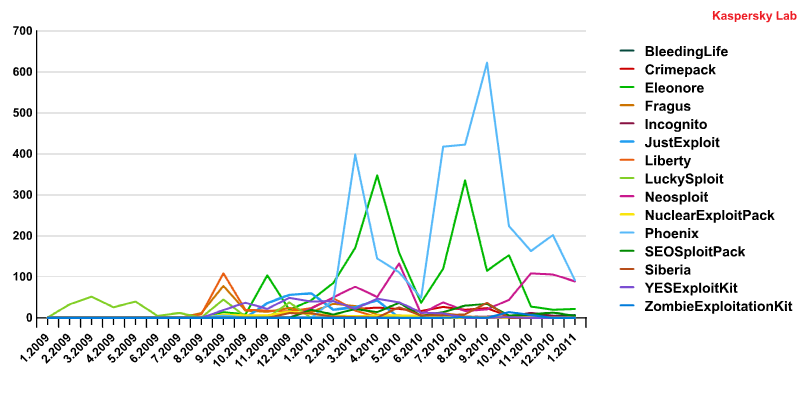
\includegraphics[scale=0.5]{Figures/kit.png}
\caption{L'évolution des kits d'exploitation.}
\label{fig :kit} 
\end{center}
\end{figure}
La figure~\ref{fig :kits} montre les vulnérabilités ciblées par ces kits d'exploitation :
\begin{figure}[H]
\begin{center}
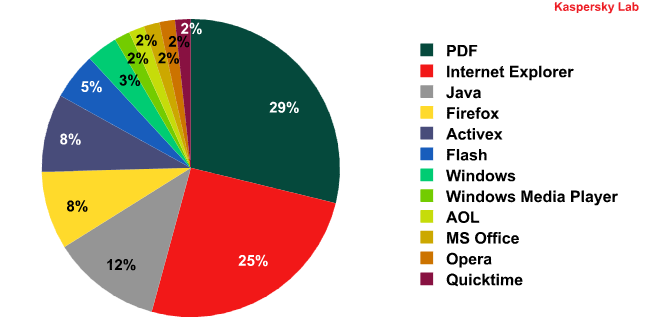
\includegraphics[scale=0.5]{Figures/kits.png}
\caption{Les vulnérabilités ciblées par les kits d'exploitation.}
\label{fig :kits} 
\end{center}
\end{figure}
Les vulnérabilités d’Internet Explorer, PDF et Java représentent 66\% des vecteurs d'attaque utilisés par les kits d'exploitation les plus répandus.
\subsection{ Les cycles de vie d'un malware}
Si on ignore la phase de conception et de test, par le créateur du malware,trois phases dans la vie d'un malware peuvent être identifiées. Leurs durées de vie respectives peuvent être plus ou moins longues, selon le type de malware et l'effet recherché.
\subsubsection{La phase d'infection}
Durant cette phase, le malware va se propager dans l'environnement informatique cible. Cela peut se produire de deux manières :
\begin{itemize}
\item Passivement : le malware est copie sur un support (disquette, CDROM , clef USB, site de téléchargement, forum de discussion... ) et transmis. Les victimes peuvent alors le copier dans leur propre environnement, avant de l'exécuter. 
\item Activement : l'utilisateur exécute le malware (cas de la première infection dans le système, appelée primo-infection) ou un fichier déjà contaminé lors d'une infection antérieure (primo-infection ou non).
\end{itemize}

\subsubsection{La phase d'incubation}
Cette phase constitue la plus grande partie de la vie d'un malware. La mission principale de cette phase est d'assurer la survie du malware, à travers toutes ses copies dans l'environnement cible. Il s'agit de limiter, voire  d'empêcher, sa détection:
\begin{itemize}
\item soit par l'utilisateur : en particulier, la phase de conception veillera tout particulièrement a éviter les erreurs d'exécution qui pourraient alerter l'utilisateur 
\item soit par l'antivirus : dans cette optique, le malware va développer plusieurs techniques qui vont lui permettre de se dérober à la surveillance antivirale.
\end{itemize}

\subsubsection{La phase de maladie}
Lors de cette phase, la charge finale est activée. Son mode de déclenchement peut dépendre de nombreux facteurs et sera fonction de l'endroit, dans le code, où la routine offensive sera placée :
\begin{itemize}
\item En tête de code, la charge finale sera systématiquement exécutée, avant
toute infection. Ce cas est rare, il a pour conséquence de limiter généralement la phase de survie du malware.
\item En fin de code, elle n'aura lieu qu'après les processus d'infection ;
\item Au milieu du code, en particulier si elle est conditionnée par la réussite
ou non de l'infection. 
\end{itemize}


\subsection{Les principales sources d'infection}
La plupart des sources d'infection sont les suivantes :\\


\begin{itemize}
\item \textbf{Internet :}Le réseau d'information global est la principale source de propagation de tout type de malware. En règle générale les virus et autres programmes malveillants sont situés sur des sites Web, déguisés sous forme de logiciels libres et utiles\\


\item \textbf{Le courrier électronique :}Les mails reçus par l'utilisateur stockés dans les bases de messagerie, peuvent aussi bien contenir des virus. Le malware peut être soit en pièce jointe ou être présent dans le corps d'un message. les données seront infectés, soit lors de l'ouverture du message ou lors de la sauvegarde sur un disque. Le courrier peut aussi être la source de deux autres menaces : le spam et le phishing. Si le spam causes principalement une perte de temps, le but du phishing est de récuperer la confidentialité des informations (par exemple numéro de carte de crédit)\\


\item \textbf{Vulnérabilités de logiciels :} Les vulnérabilités accordent aux hackers l'accès à distance, et donc aux données personnelles, aux ressources réseau via le LAN/Ethernet, et d'autres sources d'information\\


\item \textbf{Support amovible :} les disques amovibles sont largement utilisés pour transférer les informations, tel que les flash disk et les disques durs. Lors de l'ouverture d'un fichier enregistré sur un disque amovible, il peut endommager les données sur le système par un virus, et le diffuser sur d'autres lecteurs. 
\end{itemize}
\subsection{L'évolution des malwares}
\subsubsection{Tableau historique des malwares}
Le tableau \ref{malware} donne une liste des malwares les plus connus.
\begin{table}[H]
\begin{tabular}{|p{1.5cm}|p{2cm}|p{2cm}|p{9cm}|}
\hline \textbf{Date} &  \textbf{Nom} & \textbf{Type} & \textbf{Effets} \\
\hline 1986 & Brian & Virus & Infection du système de démarrage de la disquette et corruption des données de la disquette \\
\hline 1987 & Jerusalem & Virus & Infection et destruction de fichiers .exe et .com, résidant en mémoire\\
\hline 1988 & Morris Worm & Ver & Premier ver écrit pour Internet, infectant les ressources machines de l'utilisateur \\
\hline 1991 & Michelangelo & Bombe logique & Ecrasement des 256 premiers secteurs du disque dur le 6 mars 1991 \\
\hline 1999 & Melissa & Macro-virus & Via un fichier Word contaminé, la machine envoie par courrier électronique aux 50 premières adresses électroniques trouvées le fichier infecté\\
\hline 2000 & I love you & ver & Envoi massif du ver à tous les contacts Outlook, infection et corruption de fichiers et de bases de registres \\
\hline 2001 & Naked & Virus & Animation en Flash, présentant une femme nue, se diffusant à l'ensemble du carnet d'adresse et supprimant les répertoires Windows et systèmes \\
\hline 2002 & BugBear & Ver avec keylogger intégré & Installation d'un logiciel espion et envoie des enregistrements de frappes de clavier sur un serveur distant \\
\hline
\end{tabular}
%\caption{Tableau historique des malwares part 1}
\label{malware}
\end{table}
\begin{table}[H]
\begin{tabular}{|p{1.5cm}|p{2cm}|p{2cm}|p{9cm}|}
\hline \textbf{Date} &  \textbf{Nom} & \textbf{Type} & \textbf{Effets} \\
\hline 2003& Blaster & ver & Il fut aperçu pour la première fois dans la nature le 11 août. Sa vitesse de propagation augmenta exponentiellement jusqu'à atteindre un pic le 13 août. Le but de ce ver était de lancer une attaque en déni de service de type SYN flood. Pour se propager, le ver utilisait une vulnérabilité de type dépassement de tampon dans le service DCOM RPC, affectant le système d'exploitation dans son intégralité \\
\hline 2004 & Sasser & ver & il profite d'une vulnérabilité LSASS de Microsoft Windows pour télécharger sur la machine infectée un fichier nommé avserve.exe dans le répertoire Windows via FTP et le port TCP 5554 et lance son exécution à distance sans aucune intervention de l'utilisateur\\
\hline 2005 & GPCode  & Ransomware & Chiffrait les fichier et proposait à l'utilisateur de déchiffrer les fichiers en échange de 300\$\\
\hline 2006 & Nyxem & Ver avec bombe logique & Mass mailer qui supprimait les documents  Office, modifiant les paramètres systèmes, désactivant les antivirus, prévu pour s'exécuter le 3 février \\
\hline 2007 & Storm & Trojan & Dissimulé dans une pièce jointe, infection de la machine et transformation en zombie \\
\hline 2008 & Conficker& Ver & Ce ver exploite une vulnérabilité du Windows Server Service utilisé par Windows 2000, Windows XP, Windows Vista, Windows 7, Windows Server 2003 et Windows Server 2008\\
\hline 2009 & Psyb0t & Virus & Infection des routeurs DSL pouvant être manipulés sans mot de passe en raison d'un firmware trop vieux et transformation en zombie \\
\hline 2010 & Stuxnet & Ver & Stuxnet est un ver informatique supposé développé conjointement par les États-Unis et Israël pour s'attaquer à des systèmes iraniens. Spécifique au système Windows. La complexité du ver est très inhabituelle pour un malware. Il a été décrit par différents experts comme cyber arme, conçue pour attaquer une cible industrielle déterminée. Il s'agirait d'une première dans l'histoire. \\
\hline 2010 & Zeus/Zitmo & Trojan & interceptait les informations bancaires, découvert en 2007 mais une nouvelle variante voit le jour en 2010 en s'attaquant aux terminaux mobiles ainsi qu'aux consoles de jeux vidéo \\
\hline 2011 & DuQu & virus & Une vulnérabilité de Windows a été utilisée par des pirates pour mettre au point le virus DuQu, repéré le mois dernier. De façon classique, ce virus se transmet par courrier électronique dans un document Word infecté. Une fois l'ordinateur contaminé, les pirates peuvent prendre le contrôle de la machine à distance. Il aurait été créé par le même groupe à l'origine de Stuxnet\\
\hline
\end{tabular}
%\caption{Tableau historique des malwares}
\label{malware}
\end{table}
\begin{table}[H]
\begin{tabular}{|p{1.5cm}|p{2cm}|p{2cm}|p{9cm}|}
\hline \textbf{Date} &  \textbf{Nom} & \textbf{Type} & \textbf{Effets} \\
\hline 2012 & Flame & Virus & Considéré comme le descendant plus perfectionné que Stuxnet, il vise également les systèmes industriels sensibles, intercepte les données et exploite les vulnérabilités des machines Windows\\

\hline
\end{tabular}
\caption{Tableau historique des malwares}
\label{malware}
\end{table}

La figure \ref{fig :mal} montre que le nombre de malwares, entre 2005 et 2014, est dans une augmentation continue. \begin{figure}[H]
\begin{center}
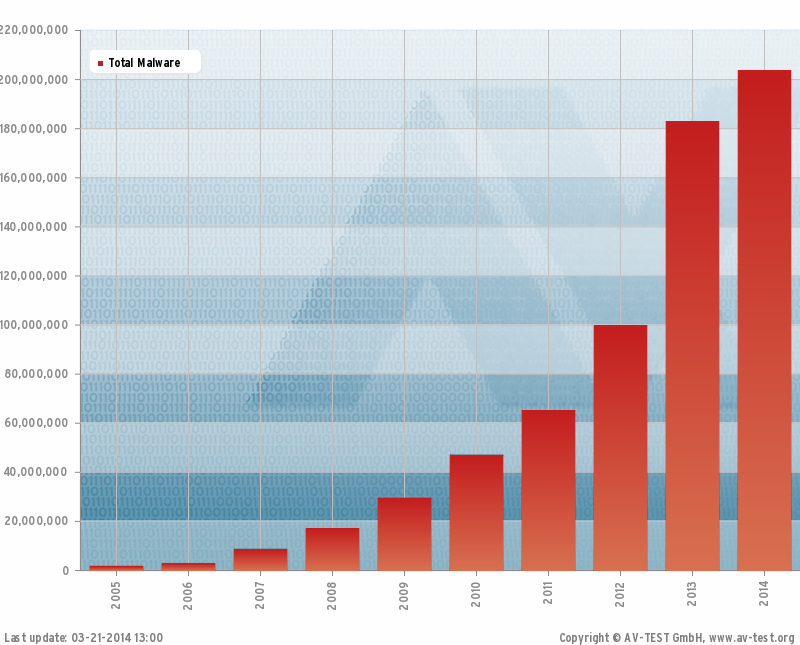
\includegraphics[scale=0.4]{Figures/mal.PNG}
\caption{nombre de malwares les dix dernières années}
\label{fig :mal} 
\end{center}
\end{figure}
\subsubsection{Evolution des malwares sur mobiles} 
Le nombre de malwares sur mobiles conçues pour des attaques de phishing, le vol de coordonnées de carte bancaire et d’argent sur les comptes en banque, a quasiment été multiplié par 20.\\

les mails sont aussi une source pour infecter les terminaux mobiles. les postes infectés forcent aussi l'utilisateur a télécharger et installer une application mobile malveillante sur son terminal. pour effectuer une fraude bancaire, la quasi totalité des banques envoient un code de sécurité par SMS à l'utilisateur. Le malware sur mobile a pour objectif d'intercepter et transférer ce code au cybercriminel, autrement il ne pourrait pas effectuer des virements bancaires à l'aide des identifiants de la victime. cette technique s'appelle "MITMO" : Malware In The MObile.\\


Les chevaux de Troie bancaires sont de loin les plus dangereux. Entre janvier et décembre 2013, leur nombre s’est multiplié. Kaspersky Lab dénombrait 67 chevaux de Troie bancaires connus début 2013, et à la fin de cette année-là, la base de données de Kaspersky Lab contenait déjà 1 321 variantes.\\


Les cybercriminels recourent de plus en plus à la technique d'obfuscation , qui consiste à rendre délibérément le code malveillant très complexe et donc plus difficile à analyser. Une solution antivirus mettra alors plus de temps à neutraliser le code laissant assez de temps aux cybercriminels pour arriver à leurs fins.\\


Parmi les méthodes pour infecter un mobile, on compte désormais la contamination via des sites légitimes compromis. La propagation du malware se fait par l'intermédiaire d’\textbf{app stores}  alternatifs et de bots (ces derniers s'autopropagent généralement par l'envoi des sms, contenant un lien malveillant, aux destinataires qui figurent dans le répertoire de la victime).\\

\subsubsection{2013 en chiffres}
Si l’on regarde 2013 de plus prêt, il est possible de constater l’énorme augmentation qu’ont connue les malwares mobiles. Néanmoins, bien que les malwares aient réussi à atteindre des sommets.
\begin{itemize}
\item En 2013, 3 905 502 paquets d’installations ont été utilisés par les cybercriminels pour distribuer les malwares mobiles
\item  les terminaux Android sont la cible priviligiée voire unique des malwares pour mobiles. Selon le rapport annuel 2014 de Cisco sur la sécurité ~\cite{cisco}, ces logiciels malveillants ciblent à 98\% les appareils Android. Sur cette plateforme, le malware mobile le plus répandu, à 43,8 pour cent, est \textbf{\textit{Andr/Qdplugin}} ~\cite{cisco}. voire figure ~\ref{fig :mobile}
\begin{figure}[H]
\begin{center}
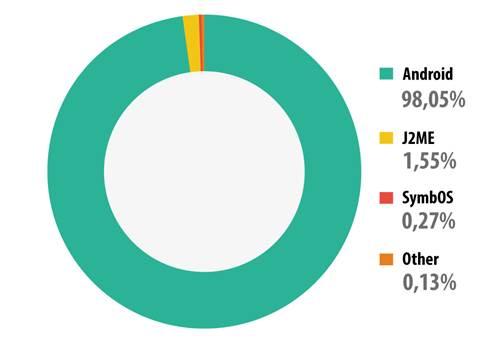
\includegraphics[scale=0.7]{Figures/mobile.jpg}
\caption{les plateformes ciblés par des malwares mobiles}
\label{fig :mobile} 
\end{center}
\end{figure}

\item La majorité des malwares mobiles(figure ~\ref{fig :mobile2}) est toujours spécialisée en vols d’argent mineurs grâce à des appels et à des messages vers des numéros surtaxés. Cependant, au cours de l’année, le nombre de modifications de malwares mobiles conçues pour le phishing, le vol d’informations de cartes bancaires ou d’argent a été multiplié par 19,7.
\begin{figure}[H]
\begin{center}
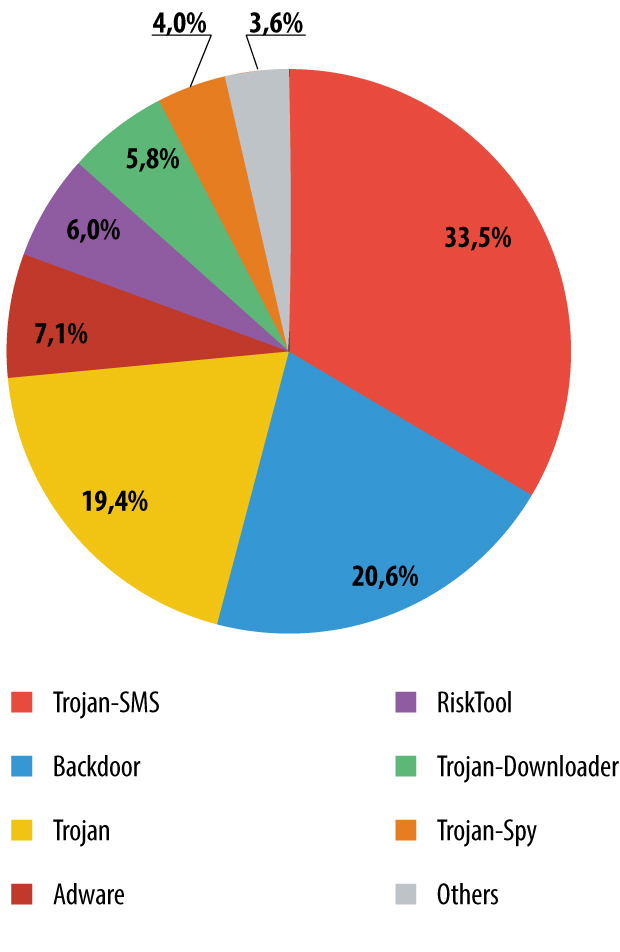
\includegraphics[scale=0.36]{Figures/mobile2.jpg}
\caption{Catégorie des malwares mobiles}
\label{fig :mobile2} 
\end{center}
\end{figure}

\end{itemize}
\subsubsection{Les malwares sur la plateforme GNU Linux}    


Le système d'exploitation Linux, au même titre que les systèmes d'exploitation Unix et apparentés, est généralement assez bien protégé contre les malwares. Cependant, certains programmes malveillants peuvent potentiellement endommager des systèmes GNU Linux non sécurisés.\\


Comme les autres systèmes Unix, Linux implémente un environnement multi-utilisateur, dans lequel les utilisateurs possèdent des droits spécifiques correspondant à leur besoin. Il existe ainsi un système de contrôle d'accès visant à interdire à un utilisateur de lire ou de modifier un fichier. Ainsi, les malwares ont typiquement moins de capacités à altérer et à infecter un système fonctionnant sous Linux que sous DOS ou encore les systèmes Microsoft Windows ayant toujours des systèmes de fichiers en FAT32 (le système de fichier NTFS a le même type de protection que les fichiers UNIX, les systèmes Microsoft Windows à base NT isolent également les comptes entre eux). C'est pourquoi, aucun des malwares écrits pour Linux, n'a pu se propager avec succès. En outre, les vulnérabilités qui sont exploitées par les malwares sont corrigées en quelques jours par les mises à jour du noyau Linux et des logiciels composant le système.\\


Des scanners du malwares sont disponibles pour des systèmes Linux afin de surveiller l'activité des malwares actifs sur Windows. Ils sont principalement utilisés sur des serveurs mandataires ou des serveurs de courrier électronique, qui ont pour client des systèmes Microsoft Windows.\\
\newpage
\textbf{\textit{Opération windigo :}}\\


Windigo est un malware qui prend la forme d’un cheval de Troie et qui se sert des serveurs Unix/Linux comme plateforme de diffusion de Spams. Différent pays sont touchés comme les USA, l'Allemagne, la France, L'Italie, la Grande Bretagne, les Pays-Bas, la Russie, l'Ukraine, le Mexique ou encore le Canada~\cite{windigo}.\\

Plus de 25000 serveurs ont été infectés par ce malware ces 2 dernières années, et plus de 10000 le sont toujours aujourd'hui. Ces serveurs sont principalement compromis par la vulnérabilité "Linux/Ebury". Le groupe à l'origine de la vulnérabilité "Linux/Ebury" est également l'auteur des vulnérabilités "Linux/Cdorked", "Perl/Calfbot" et "Win32/Glupteba.M".\\ 


Windigo s'appuie sur trois composants :
\begin{itemize}
\item \textbf{Linux/Ebury : }Backdoor OpenSSH pour garder un contrôle du serveur et pour voler les identifiants
\item \textbf{Linux/Cdorked : }Backdoor HTTP pour la redirection du trafic, ainsi qu’un serveur DNS modifié connu sous le nom de Linux/Onimiki
\item \textbf{Perl/Calfbot : }Script PERL pour générer du spam.

\end{itemize}
Les serveurs infectés redirigent plus d'un demi-million de visiteurs vers du contenu malicieux chaque jour. Ces serveurs donnent accès à une grande capacité de bande passante, de stockage, de puissance de calcul et de mémoire. Les attaquants sont capables d'envoyer plus de 35000000 pourriels par jours. Il est intéressant de noter que l'installation est faite de manière manuelle par les auteurs du malware.\\

Windigo affecte aussi bien les serveurs que les PC. Les systèmes d'exploitation affectés sont Linux, FreeBSD, OpenBSD, OS X, et même Microsoft Windows (avec Perl tournant sous Cygwin). Les serveurs cPanel et kernel.org font partie de la liste des victimes de ce malware. Il agit de différentes manières en fonction des systèmes :
\begin{itemize}

\item Sous Microsoft Windows il installe un kit d’exploitation
\item Sous MAC OS, il affiche des publicités pour des sites de rencontre
\item Sous IOS les utilisateurs sont redirigés vers des sites à contenu pornographique.

\end{itemize}
En cas d'infection, un formatage et une réinstallation complète du système sont nécessaires. la commande suivante dans un terminal permet de savoir si le système est infecté ou non :\\
\begin{lstlisting}
$ ssh -G 2>&1 | grep -e illegal -e unknown > /dev/null && echo "System clean"
 || echo "System infected"
\end{lstlisting}
\subsubsection{Les malwares sur la plateforme Mac OS X}
Nombreux sont ceux à croire que la plateforme Mac OS X de Apple est plus sécurisée que Microsoft Windows. Certains pensent que son mode UNIX pour la gestion des privilèges et des permissions lui confère une sécurité plus solide que Microsoft Windows, et sa gamme de matériel plus limitée implique moins de code et donc moins d'exposition aux vulnérabilités liées au code.\\


Pourtant, comme les Macs sont moins répandus en milieu professionnel, ils constituent une cible réduite pour les 
cybercriminels. Ceci explique que le problème des malwares sur Macs ne représente qu'une infime partie de ce que l'on peut voir sur les plateformes Microsoft Windows. Cependant, de nouveaux malwares continuent sans cesse d'émerger. Et même si
la zone d'attaques ne présente pas autant de possibilités d'infection et de propagation, les utilisateurs de Mac sont toujours vulnérables aux escroqueries et aux arnaques utilisées pour les piéger et les inciter à installer des logiciels suspects visant à accéder à leurs systèmes et à leurs données à distance.\\


Par exemple, 2010 a vu une nouvelle version du cheval de Troie OSX/Pinhead, qui se présente comme une copie de l'application iPhoto comprise avec tous les nouveaux Mac. Si l'utilisateur dupé installe le logiciel, il ouvre une porte dérobée qui donne aux pirates un plein accès au système compromis. Plus tard dans l'année, c'était au tour du cheval de Troie Boonana de viser les utilisateurs de Mac, Microsoft Windows et même GNU Linux. Il s'est propagé via des liens spammés sur Facebook et a utilisé des arnaques  classiques d'ingénierie sociale pour piéger ses victimes et leur faire installer une application Java, qui télécharge et exécute une autre série d'applications malveillantes.\\


En 2011, l'émergence des malwares Mac a attiré beaucoup d'attention. Il est évident que le problème des malwares Windows est
bien supérieur à la menace sur Mac, mais les évènements de 2011 ont rappelé aux utilisateurs Mac qu'ils devaient être
prudents. Les cybercriminels utilisent désormais les mêmes techniques sur Mac que sur PC, à savoir l'infection par les faux antivirus tels que MacDefender, Mac Security, MacProtector et MacGuard, qui sont tous apparus dans le courant de l'année.\\

Le système d'exploitation Mac OS X 10.7 d'Apple, surnommé Lion, prétend protéger l'utilisateur contre les malwares. Cependant, il ne détecte qu'un nombre limité de téléchargements malveillants issus de 10 différents types de malwares
Mac.\\


Bien que cette année la plate-forme Mac OS X n'ait pas subi d'attaque égalant l'étendue mondiale de Flashback en 2012, les attaques ont continué à évoluer en 2013, sous des formes diverses : chevaux de Troie, attaques contre les vulnérabilités de Java et les formats des documents Word, plug-ins agressifs, JavaScript malveillant et malwares conçus pour passer outre la protection Apple Gatekeeper grâce à une fausse identité Apple Developer.
\begin{figure}[H]
\begin{center}
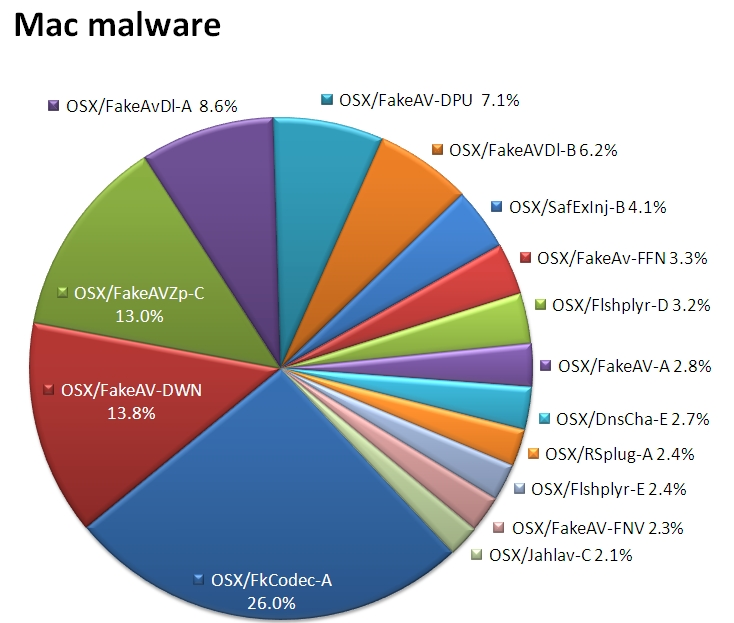
\includegraphics[scale=0.45]{Figures/mac.jpg}
\caption{Les malwares sous la plate-forme MAC OS X.}
\label{fig :kit} 
\end{center}
\end{figure}
\subsubsection{Les malwares multi-plateformes}
Récemment, les attaques contre les Mac, Facebook, Apple et Microsoft ont rappelé que les cybercriminels n'avaient pas que Microsoft Windows dans leurs lignes de mire. Et le fait de cibler deux voire plusieurs plateformes à la fois, comme le font déjà les adwares et les spams, devient de plus en plus fréquent pour les malware. En utilisant des langages de programmation multi-plateformes comme Java, les cybercriminels mettent en place des logiciels malveillants qui, en compromettant un site web, peuvent percevoir le système d'exploitation qu'utilise le visiteur. Ils y déposent un malware, affichent des publicités, redirigent l'internaute vers un site web frauduleux, tentant de générer de l'argent en s'adaptant à l'appareil servant à la connexion, quel qu'il soit.\\

Les malwares multi-plateformes, générés par la popularité des applications multi-plateformes ciblent généralement les macro des suites bureautiques, en particulier celles qui autorisent l'exécution de scripts comme ActiveX, mais cela peut se faire par l'ajout de plugins ou d'extensions provenant de sources non fiables. Cela est vrai aussi pour les navigateurs web.

\textbf{\textit{Exemples : }}\\
\begin{itemize}
\item Un botnet java multi-plateforme est utilisé dans des attaques DDOS. L'application Java malveillante peut être exécutée sur des machines Microsoft Windows, OS X et GNU Linux. L'éditeur de solutions de sécurité Kaspersky avertit sur son blog d'un nouveau malware utilisant une faille de la machine virtuelle Java. Même si la brèche a déjà été colmatée, nombreux sont les ordinateurs à posséder une ancienne mouture, ce qui rend la menace potentiellement sérieuse. Ce n'est pas la première fois qu'un botnet infecte les trois systèmes d'exploitation de bureau les plus populaires. Un côté multiplateforme que lui confère à chaque fois Java.\\


\item L'exemple le plus flagrant de malware multiplateforme est Zeus et sa version mobile Zeus-in-the-Mobile (ZitMo) qui avaient pour but de voler des données bancaires.\\
Zeus utilise un procédé assez simple. Le cheval de Troie commence par compromettre un ordinateur Microsoft Windows et attend que l'utilisateur ouvre son navigateur et accède à ses comptes en ligne. Ensuite, il ajoute des champs additionnels à la page Web de la banque, où il invite les utilisateurs à renseigner leurs numéro de téléphone ainsi que leurs modèle de téléphone mobile pour des soi-disant renouvellements de certificat. Par conséquent, les propriétaires du Zeus obtiennent toutes les informations qui ont été rentrées sur la page modifiée, y compris toutes les informations bancaires requises en ligne. Après cela, un SMS est envoyé au numéro de téléphone qu'avez renseigné : celui-ci contient un lien vers un certificat qui n'existe pas et qui est en fait le cheval de Troie, ZitMo. Une fois le smartphone infecté, le malware mobile commence à intercepter les codes d'autorisation et les notifications de mouvement sur le compte qui sont envoyés par SMS par la banque. Ainsi, sans que vous le sachiez, le cybercriminel pourra travailler à distance sur le compte bancaire de la victime en utilisant des données volées.
\end{itemize}

\section{Les Antivirus}

\subsection{Définition}
Il s'agit d'un logiciel capable de détecter et de détruire les virus contenus sur un disque. Le logiciel a pour charge de surveiller la présence de virus et éventuellement de nettoyer, supprimer ou mettre en quarantaine le ou les fichiers infectés. Ils surveillent tous les espaces dans lesquels un virus peut se loger, c'est à dire la mémoire et les unités de stockage qui peuvent être locales ou sur le réseau~\cite{anti}.
\subsection{Fonctionnement des Antivirus}
les antivirus fonctionnent à quelques rares exceptions près - selon deux modes : ~\cite{anti}
\subsubsection{Mode statique :} 
L'antivirus n'est alors actif que par une action volontaire
de l'utilisateur (déclenchement manuel ou pré-programmé), il est donc le plus souvent inactif et aucune détection n'est possible. C'est le mode le plus adapté aux machines de faible puissance. La technique de surveillance de comportement n'est pas disponible dans ce mode.\\
Notre antivirus qu'on va déployer, il sera en mode statique.
\subsubsection{Mode dynamique :}
l'antivirus est, en fait, résident et surveille en permanence l'activité du système d'exploitation, du réseau et surtout de l'utilisateur. II prend la main avant toute action et tente de déterminer si un risque viral existe, lié à cette action. Ce mode est gourmand en ressources et nécessite des machines relativement puissantes, pour ne pas être handicapant et pousser l'utilisateur (cas trop souvent rencontré) a désactiver ce mode au profit du précédent.
\subsection{Les techniques antivirales}
Les antivirus modernes, pour les plus efficaces, conjuguent plusieurs techniques afin de réduire le risque de fausses alarmes et de non-détection, au minimum. Elles peuvent être classees en deux groupes : les techniques statiques et les techniques dynamiques~\cite{anti}.
\subsubsection{Recherche de signatures}
Cette technique consiste a rechercher une suite d'octets, caractéristique d'un malware donné. Cette suite est analogue à l'empreinte digitale d'une personne. Utilisée comme signature, elle doit posséder deux propriétés importantes ~\cite{anti} :
\begin{itemize}
\item Elle doit être \textit{discriminante}. Cela signifie que la signature doit identifier spécifiquement le malware
\item Elle doit être \textit{non incriminante}. Autrement dit, elle ne doit théoriquement
pas incriminer un autre malware, ou un programme sain. Elle doit donc posséder une taille et des caractéristiques suffisamment pertinentes pour ne pas provoquer de faux positifs.
\end{itemize}

En général, plus la séquence utilisée pour définir la signature est longue, plus cette signature réalisera ces deux propriétés.\\


Cette signature peut être :
\begin{itemize}
\item soit une séquence d'instructions;
\item soit un message affiché par le malware;
\item soit tout simplement la signature que le malware lui-même utilise pour éviter la surinfection d'un exécutable.
\end{itemize}


La base de signatures comporte, pour chaque malware qui s'y trouve recensé :
\begin{itemize}
\item La signature proprement dite;
\item l'endroit où la chercher (en-tête de Inexécutable, début ou fin du code... ).
plutot que de rechercher la séquence d'octets qui la définit dans tout l'exécutable. l'antivirus se limite a une zone spécifique de cet exécutable, cela permet d'accélérer la recherche;
\item le mode de recherche : recherche simple de la signature, décompression du code, déchiffrement ...\\
\item le nom du malware : quand l'antivirus identifie une souche virale, il informe l'utilisateur en utilisant le nom du malware comme : duqu, stuxnet, conficker, blaster, sasser, zeus, ...
\end{itemize}


Si la détection par signatures peut se révéler très efficace, elle se limite aux
malwares connus et analysés. Le problème avec cette technique est qu'elle est facilement
contournable. Un simple changement de compilateur suffit à leurrer la plupart des antivirus. Elle ne permet de gérer ni les virus polymorphes, ni certains virus chiffrés, et encore moins les malwares inconnus. Le taux de faux positifs est faible bien que l'identification correcte laisse quelquefois à désirer (problème de fausse incrimination).\\

Le principal inconvénient  de ce mode de détection est la nécessité de maintenir la base de signatures virales avec les contraintes que cela comporte :taille de la base, stockage sécurisé (des sites d'antivirus contenant les bases de signatures de leurs produits sont quelquefois attaqués), la distribution sécurisée, la mise à jour plus ou moins régulière et effective par l'utilisateur, souvent négligent. A noter que la mise à
jour de ces bases permet la détection de nouveaux malwares, mais aussi, dans certains cas, d'améliorer la détection des malwares précédemment repérés (par d'autres techniques) en diminuant, par exemple, les ressources machine nécessaires.\\
\subsubsection{Analyse spectrale}
L'analyse spectrale repose sur le postulat que tout code généré automatiquement contiendra des signes révélateurs du compilateur utilisé. De même, on part du principe qu'il est impossible de retrouver dans un vrai programme exécutable compilé certaines séquences de code. L'analyse spectrale vise donc elle aussi à repérer les virus polymorphes ou inconnus. Lorsqu'un virus polymorphe chiffre son code, la séquence en résultant contient certaines associations d'instructions que l'on ne trouverait pas dans un vrai programme. C'est ce que l'analyse spectrale tente de détecter. Par exemple, si dans un programme exécutable, l'antivirus trouve une instruction de lecture d'un octet au delà de la taille limite de la mémoire, on sera
probablement en présence de code chiffré, packé ou polymorphe~\cite{anti}.\\
\subsubsection{Contrôle d'intégrité}
Puisque les virus modifient les programmes qu'ils infectent, certains antivirus utilisent un contrôleur d'intégrité pour vérifier si les fichiers de la machine ont été modifiés. Ainsi, une base de données est construite, qui contient des détails sur les fichiers exécutables du système, comme leur taille ou leur date de modification, et éventuellement un condensé cryptographique (checksum).. Dès lors, si une de ces caractéristiques change pour un exécutable, l'antivirus s'en aperçoit~\cite{antiv}.

\subsubsection{La surveillance comportementale}
L'antivirus est résident en mémoire et tente d'identifier tout comportement suspect (la définition d'un tel comportement se faisant par rapport à une base de comportements viraux) et le bloquer si nécessaire.
Les actions suivantes peuvent être identifiées comme malveillantes : tentatives d'ouvertures en lecture/écriture de fichiers exécutables, écriture sur des secteurs systèmes (partition ou démarrage), tentative de mise en résident, etc.\\
Techniquement, l'antivirus agit par détournement d'interruptions (le plus souvent, les interruptions 13H et 21H) ou d'API.\\
Cette technique permet de détecter quelquefois des malwares inconnus (utilisant cependant des techniques connues) et de lutter avant l'infection. Toutefois, certaines techniques virales y échappent. De plus, l'antivirus doit être en mode dynamique, ce qui ralentit, quelquefois sensiblement, le système. Les faux positifs sont relativement nombreuses. Notons que l'analyse de l'antivirus permet de connaitre la base de comportements et tout le jeu du
programmeur du malware consistera à utiliser cette connaissance pour mieux contourner la protection~\cite{anti}.


\subsubsection{L'émulation de code}
Cette technique permet de disposer de la surveillance de comportement en mode statique, ce qui est assez utile car beaucoup d'utilisateurs impatients préfèrent ce mode pourtant dangereux. Lors du scan, le code étudié est chargé dans une zone memoire confinée, puis est émulé afin de détecter un comportement potentiellement viral. L'émulation de code est particulièrement
adaptée à la lutte contre les virus polymorphes. Cette technique souffre toutefois des mêmes limitations que son homologue dynamique~\cite{anti}.
\subsection{Eradication des malwares}
\subsubsection{Méthode d'éradication}
Une fois un malware détecté, il faut le supprimer. Mais il n'est pas toujours simple de supprimer un malware  sans endommager le programme original. En effet, certains programmes malicieux  détruisent une partie du programme sain lors de leur duplication. Il ne reste plus alors qu'à détruire purement et simplement le fichier infecté. Dans les autres cas, la suppression d'un malware n'est pas forcément évidente non plus. Il s'agit d'abord de découvrir très précisément où est localisé le malware dans le fichier, sachant qu'il peut être composé de plusieurs parties. Il faut ensuite supprimer ces octets infectés, et récupérer la partie du programme dont le malware avait pris la place, afin de la restaurer. Toutes ces manipulations nécessitent bien sûr une parfaite connaissance du malware et de son mode opératoire. C'est à cela que servent les fichiers de signatures des antivirus, régulièrement remis à jour. Il faut non seulement pouvoir détecter le virus, mais aussi savoir où il cache la portion de code dont il a pris la place~\cite{antiv}.
\subsubsection{Mise à jour des antivirus}
Cela pose donc la problématique de la mise à jour rapide des antivirus, et donc de la mise à disposition rapide des signatures de détection et méthodes de désinfection.\\


L'efficacité des solutions antivirus dépend des bases de données de définitions du malware. Ces bases sont dynamiques par nature étant donné la constante activité des auteurs des malwares. Par exemple, les analystes viraux de Kaspersky Lab détectent et ajoutent 100 nouvelles menaces quotidiennement à la base antivirus.\\


Les antivirus sont devenus de plus en plus sophistiqués au fil des années afin de contrer la complexité croissante des programmes malicieux. Des mécanismes de protection proactifs, heuristiques, conçus pour détecter les nouvelles menaces avant qu'elles n'apparaissent dans la nature offrent une première ligne de défense importante.\\


Néanmoins, une mise à jour régulière de la protection antivirus est plus importante que jamais étant donné la rapidité à laquelle les menaces actuelles sont capables de se propager. Les éditeurs d'antivirus ont réduit l'intervalle entre les mises à jour de signatures de trimestriellement à mensuellement et finalement à quotidiennement. Malgré toutes ces bonnes intentions, rien ne garantit que l'utilisateur final effectuera des mises à jour assez régulières. Ni qu'un virus à propagation rapide n'aura pas déjà infecté les machines avant la mise à disposition de mise à jour~\cite{antivirus}.
\section{Le besoin de l'analyse des malwares}
Tout comme l'écriture de code malveillant, il y a une myriade de raisons d'analyser les virus, les vers et les trojans. La raison principale derrière cela est qu'il n'y a aucun code source disponible pour de tels programmes. Le seul
moyen de comprendre ces programmes est de les analyser et déterminer leur fonctionnement interne. Une autre raison pourrait être que beaucoup de chercheurs aiment explorer les fonctionnements cachés d'un programme en l'examinant avec un désassembleur et un débogueur.\\


Il y a deux techniques majeures pour analyser ce code :\\

\begin{itemize}
\item \textbf{\textit{l'analyse statique : }}L'analyse statique de malwares consiste à explorer le contenu des fichiers suspects à l'aide de divers outils, dans le but d'extraire le maximum d'informations sans exécuter le code malveillant qu'ils pourraient contenir. A ce stade il s'agit uniquement d'observer le contenu "visible"\\
\item \textbf{\textit{l'analyse dynamique : }}Contrairement à l'analyse statiques, l'analyse dynamique consiste à exécuter réellement le code malveillant dans un environnement adéquat afin d'observer toutes ses actions et d'en déduire son comportement global. Ce type de méthode est parfois appelée analyse comportementale.\\

\end{itemize}


Ces deux techniques seront discutées dans le chapitre 5.
\section{Conclusion}
Tout au long de ce chapitre, une problématique majeure de la sécurité informatique a été abordée : les malwares.
Il a été constaté qu'il existait plusieurs types de malware, tel que les virus, les vers, les trojans ...\\


Les éditeurs d'antivirus ont donc de beaux jours devant eux, leur fond de commerce n'étant pas prêt de disparaître. Il leur faut néanmoins travailler d'arrache-pied pour trouver (ou améliorer) de nouvelles solutions pour combattre ce
fléau. Car, à chaque innovation des antivirus, les virus franchissent eux aussi un cap. Avec un avantage majeur à l'heure actuelle : il faut qu'ils soient découverts avant de pouvoir être combattus...\\


Si, aujourd'hui, Microsoft Windows est le système d'exploitation majoritairement touché, il est à craindre qu'avec l'explosion de GNU Linux et Apple Mac OS, et son arrivée imminente dans un plus grand nombre de foyers, fasse augmenter les attaques tournées vers ces systèmes. Surtout si des utilisateurs moins expérimentés viennent à l'utiliser. Il a cependant
une bonne marge d'avance, puisque le nombre de virus en activité sous Linux est dérisoire par rapport à ceux pour l'OS de Microsoft.\\


Dans le chapitre suivant on va parler sur les fichiers de format PE (Portable exécutable) 
de Microsoft Windows avec détailles parce que les antivirus doivent être capable de parser le format PE afin de pouvoir appliquer les différentes méthodes de détection (signature, émulation de code, ...). Aussi a connaissance du format PE est importante pour l'analyste afin de mieux comprendre et analyser manuellement le malware.
\chapter{Etude du format PE}

\section{Introduction au format Portable Executable}
Le format PE (Portable Executable), est un format du fichier natif spécifique à Microsoft Windows, qui structure les fichiers exécutable du système d'exploitation. Développé par Microsoft, et dérivé d'Unix COFF (Common Object File Format), ce format structure les binaires à extension *.exe (Logiciel), *.ocx (Object Linking and Embbeding), *.dll (Dynamic Link Library) et *.cpl (Panneau de Configuration) sur toutes les plateformes Win32 et supérieur~\cite{wiki}.
\\

D'un point de vue sécuritaire, la connaissance de ce format est en soit une base qu'il est nécessaire de posséder lorsque l'on souhaite se lancer dans la conception et développement d'un parseur de PE.
\section{Bref historique}
Microsoft migra vers le format PE avec l'introduction de Microsoft Windows NT 3.1. Toutes les versions suivantes de Microsoft Windows, incluant Microsoft Windows 95/98/ME, supportent ce format. Auparavant les fichiers avec \og exécutable \fg. étaient au format NE \og Executable File Format \fg.\\
 La création du format PE a été induite par le fait que Microsoft souhaitait créer une structure du fichier portable, de sorte qu'elle puisse s'adapter aux différents systèmes de Microsoft Windows NT, car il faut savoir que Microsoft Windows NT était au départ capable de supporter d'autres architectures que le x86 d'Intel, Power PC et Motorola 68000 en faisaient partie~\cite{MS}.
\\
L'idée fût donc de créer une structure commune à ces architectures.
\section{Schéma du format PE}
PE étant une structure du fichier, cela signifie qu'il est formaté d'une certaine façon. La figure~\ref{fig :PEX} montre son formatage :
\begin{figure}[H]
\begin{center}
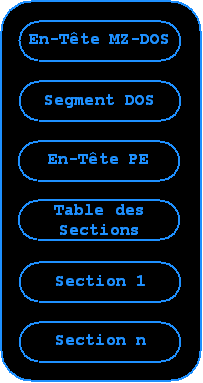
\includegraphics[scale=0.6]{Figures/PE.png}
\caption{Organisation générale d'un fichier PE}
\label{fig :PEX} 
\end{center}
\end{figure}

Tous les fichiers PE respectent ce formatage. Si on essaye, par exemple, d'ouvrir un fichier *.exe avec un éditeur hexadécimal on s'aperçoit que les deux premiers octets sont MZ, qui correspondent bien aux 2 premiers octets de l'en-tête MZ-DOS décrit ci-dessous.
\subsection{En-tête MZ-DOS}
L'en-tête MZ-DOS permet au système d'exploitation de reconnaître le fichier comme étant un exécutable valide dans le cas où celui-ci serait lancé depuis MS-DOS,afin de pouvoir exécuter son segment DOS. Cet en-tête est également soumis à une structuration, nommée IMAGE\_DOS\_HEADER, cette structure permet de formater l'en-tête MZ-DOS. Ci-dessous, son prototype en langage C.
\begin{lstlisting}
typedef struct _IMAGE_DOS_HEADER { // DOS .EXE header
WORD e_magic;                      // Magic number
WORD e_cblp;                       // Bytes on last page of file
WORD e_cp;                         // Pages in file
WORD e_crlc;                       // Relocations
WORD e_cparhdr;                    // Size of header in paragraphs
WORD e_minalloc;                   // Minimum extra paragraphs needed
WORD e_maxalloc;                   // Maximum extra paragraphs needed
WORD e_ss;                         // Initial (relative) SS value
WORD e_sp;                         // Initial SP value
WORD e_csum;                       // Checksum
WORD e_ip;                         // Initial IP value
WORD e_cs;                         // Initial (relative) CS value
WORD e_lfarlc;                     // File address of relocation table
WORD e_ovno;                       // Overlay number
WORD e_res[4];                     // Reserved words 
WORD e_oemid;                      // OEM identifier (for e_oeminfo)
WORD e_oeminfo;                    // OEM information; e_oemid specific
WORD e_res2[10];                   // Reserved words
LONG e_lfanew;                     // File address of new exe header
} IMAGE_DOS_HEADER, *PIMAGE_DOS_HEADER;
\end{lstlisting}
\newpage
La figure~\ref{fig :pic1} montre un exemple réel avec le parseur CFF Explorer :
\begin{figure}[H]
\begin{center}
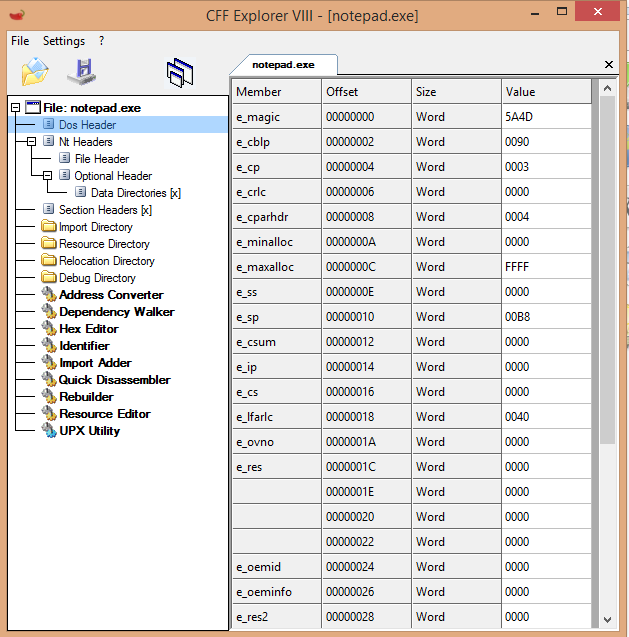
\includegraphics[scale=0.7]{Figures/pic1.PNG}
\caption{ En-tête MZ-DOS d'un fichier PE avec CFF Explorer.}
\label{fig :pic1} 
\end{center}
\end{figure}
les champs les plus importants sont :
\begin{itemize}
\item \textbf{e\_magic : }qui doit valoir "MZ"
\item \textbf{e\_lfanew : }contient l'adresse du début de l'en-tête PE.
\end{itemize}
\subsection{Segment DOS}
Le segment DOS est exécuté lorsque l'application est lancée sous MS-DOS au lieu d'un environnement fenêtré Microsoft Windows, il affiche en général un message comme "This program must be run under Win32", autrement dit "Ce programme doit être exécuté sous Win32". Il s'agit d'un message implémenté par le compilateur, lors de la compilation du code logiciel, et dans le plupart des cas une exécution de int 21h, une interruption du BIOS (Basic Input Ouput System) qui permet d'afficher un texte à l'écran.\\


La figure~\ref{fig :pic2} montre l'ouverture d'un fichier PE avec éditeur hexadécimal.
\begin{figure}[H]
\begin{center}
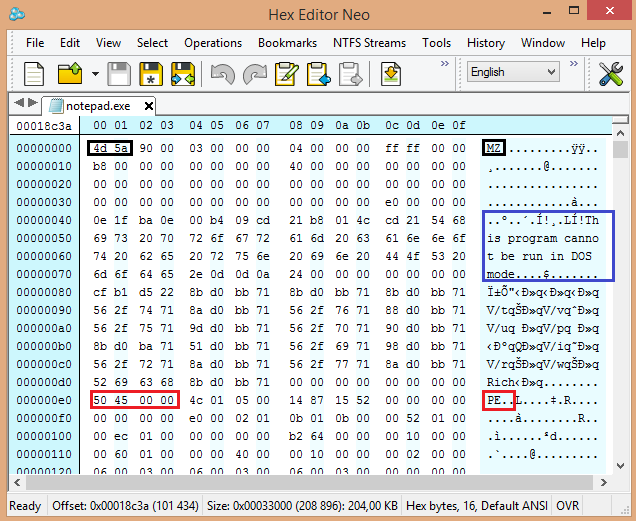
\includegraphics[scale=0.8]{Figures/pic2.PNG}
\caption{ Segment DOS d'un fichier PE avec Hex Editor.}
\label{fig :pic2} 
\end{center}
\end{figure}
\subsection{En-tête PE}
L'en-tête PE est un ensemble de structures, regroupées dans une même et unique nommé IMAGE\_NT\_HEADER,
voici son prototype en langage C.
\begin{lstlisting}
typedef struct _IMAGE_NT_HEADERS {
DWORD                 Signature;
IMAGE_FILE_HEADER     FileHeader;
IMAGE_OPTIONAL_HEADER OptionalHeader;
}IMAGE_NT_HEADERS, *PIMAGE_NT_HEADERS;
\end{lstlisting}


Le premier champ,\textbf{Signature : }signature Signature permettant d'identifier le fichier, qui doit être égale à 0x00004550, soit "PE00". (voire la figure~\ref{fig :pic2} qui est en rouge).
\\
\subsection{L'en-tête du fichier}

L'en-tête du fichier est une structure nommé IMAGE\_FILE\_HEADER, qui contient les informations
concernant la structuration du fichier. Elle est prototypée comme suit :
\begin{lstlisting}
typedef struct _IMAGE_FILE_HEADER {
WORD   Machine;                       
WORD   NumberOfSections;
DWORD  TimeDateStamp;
DWORD  PointerToSymbolTable;
DWORD  NumberOfSymbols;
WORD   SizeOfOptionalHeader;
WORD   Characteristics;
}IMAGE_FILE_HEADER, *PIMAGE_FILE_HEADER;
\end{lstlisting}
Le Tableau~\ref{tab1} explique les champs de la structure IMAGE\_FILE\_HEADER:
\begin{table}[h]
\begin{tabular}{|p{4.5cm}|p{10.5cm}|}
\hline \textbf{champ} &  \textbf{contenu}\\
\hline Machine & Le processeur pour lequel le fichier est prévu.\\
\hline NumberOfSections & Le nombre de sections dans le fichier.\\
\hline TimeDateStamp & La date et l'heure auxquelles le fichier a été créé.\\
\hline PointerToSymbolTable & Utilisé pour le débogage. Semble être toujours 0.\\
\hline NumberOfSymbols & Utilisé pour le débogage. Semble être toujours 0.\\
\hline SizeOfOptionalHeader & Taille de la structure OptionalHeader.\\
\hline Characteristics & Contient des flags pour le fichier.\\
\hline
\end{tabular}
\caption{La structure de l'en-tête du fichier PE}
\label{tab1}
\end{table}
Exemple réel avec CFF Explorer (figure~\ref{fig :pic3} ) :
\begin{figure}[H]
\begin{center}
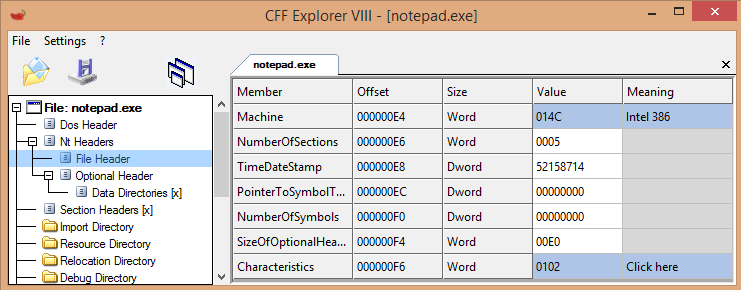
\includegraphics[scale=0.7]{Figures/pic3.PNG}
\caption{ L'en-tête du fichier PE avec CFF Explorer.}
\label{fig :pic3} 
\end{center}
\end{figure}

\subsection{L'en-tête facultatif}

L'en-tête facultatif est le dernier membre de la structure IMAGE\_NT\_HEADER. Il contient des informations sur l'organisation logique du fichier PE~\cite{PE}.
Il est prototypé comme suit :
\begin{lstlisting}

typedef struct _IMAGE_OPTIONAL_HEADER {
  WORD                 Magic;
  BYTE                 MajorLinkerVersion;
  BYTE                 MinorLinkerVersion;
  DWORD                SizeOfCode;
  DWORD                SizeOfInitializedData;
  DWORD                SizeOfUninitializedData;
  DWORD                AddressOfEntryPoint;
  DWORD                BaseOfCode;
  DWORD                BaseOfData;
  DWORD                ImageBase;
  DWORD                SectionAlignment;
  DWORD                FileAlignment;
  WORD                 MajorOperatingSystemVersion;
  WORD                 MinorOperatingSystemVersion;
  WORD                 MajorImageVersion;
  WORD                 MinorImageVersion;
  WORD                 MajorSubsystemVersion;
  WORD                 MinorSubsystemVersion;
  DWORD                Win32VersionValue;
  DWORD                SizeOfImage;
  DWORD                SizeOfHeaders;
  DWORD                CheckSum;
  WORD                 Subsystem;
  WORD                 DllCharacteristics;
  DWORD                SizeOfStackReserve;
  DWORD                SizeOfStackCommit;
  DWORD                SizeOfHeapReserve;
  DWORD                SizeOfHeapCommit;
  DWORD                LoaderFlags;
  DWORD                NumberOfRvaAndSizes;
  IMAGE_DATA_DIRECTORY DataDirectory[IMAGE_NUMBEROF_DIRECTORY_ENTRIES];
} IMAGE_OPTIONAL_HEADER, *PIMAGE_OPTIONAL_HEADER;
\end{lstlisting}


Cette structure comporte 31 champs. Certains d'entre eux sont cruciaux et d'autres ne sont pas utiles. Nous verrons uniquement les champs qui sont réellement utiles.\\
Exemple réel avec CFF Explorer (voire figure~\ref{fig :pic4}) :
\begin{figure}[H]
\begin{center}
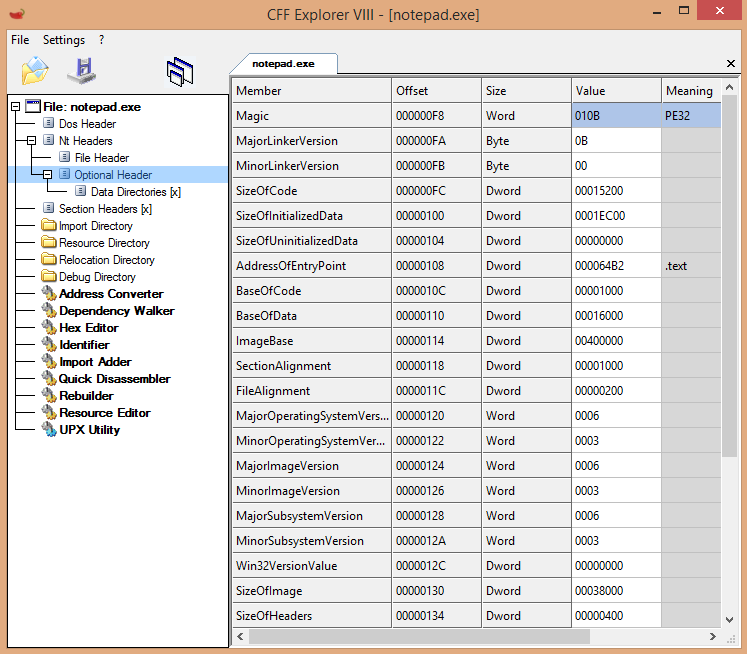
\includegraphics[scale=0.7]{Figures/pic4.PNG}
\caption{ L'en-tête facultatif d'un fichier PE avec CFF Explorer.}
\label{fig :pic4} 
\end{center}
\end{figure}


Un mot revient fréquemment en relation avec le format PE : \textbf{RVA}.\\
RVA signifie Relative Virtual Address. RVA est un terme un peu rebutant pour un concept aussi simple. Pour parler simplement, une RVA est une distance à partir d'un point de référence dans l'espace d'adressage virtuel. Une RVA est exactement la même chose qu'un offset fichier. Toutefois, elle est relative à une adresse virtuelle plutôt qu'au début d'un fichier.\\
Voici un exemple :\\
Si un fichier PE est chargé à l'adresse \$400000 dans l'espace d'adressage virtuel et que le programme commence son exécution à l'adresse \$401000, on peut dire que le programme débute à la RVA \$1000. Une RVA est relative à l'adresse virtuelle du premier octet du module.\\
Pourquoi le format PE utilise-t-il des RVA ? Le but est de réduire le temps de chargement du PE Loader. Sachant qu'un module peut être déplacé n'importe où dans l'espace d'adressage virtuel, ce serait infernal pour le PE Loader de fixer les adresses de chaque élément à position variable du module. Par opposition, si tous les éléments ayant une position variable dans le fichier utilisent des RVA, le PE Loader n'a alors pas besoin de fixer quoi que ce soit : il déplace simplement tout le module à une nouvelle adresse virtuelle. Tout cela rejoint le concept de chemin relatif et chemin absolu : une RVA est assimilable à un chemin relatif, une adresse virtuelle à un chemin absolu.\\

Voici le tableau~\ref{tab2} qui donne les champs intéressants de l'en-tête facultatif : 

\begin{table}[h]
\begin{tabular}{|p{4.5cm}|p{11cm}|}
\hline \textbf{champ} &  \textbf{contenu}\\
\hline AddressOfEntryPoint & Il s'agit de la RVA de la première instruction qui sera exécutée lorsque le PE Loader sera prêt à lancer le fichier.\\
\hline ImageBase &	C'est l'adresse de chargement souhaitable pour le fichier PE.\\
\hline SectionAlignment & La granularité de l'alignement des sections en mémoire.\\
\hline FileAlignment & La granularité de l'alignement des sections dans le fichier.\\
\hline MajorSubSystemVersion & La version du système Win32.\\
\hline MinorSubSystemVersion & La version du système Win32.\\
\hline SizeOfImage & La taille totale du fichier PE en mémoire. C'est la somme de tous les en-têtes et des sections alignées avec la valeur SectionAlignment.\\
\hline SizeOfHeaders & La taille de tous les en-têtes et de la table des sections. Cette valeur est égale à la taille du fichier moins la taille de toutes les sections.\\
\hline Subsystem & Donne pour quel sous-système NT le fichier PE est prévu.\\
\hline DataDirectory & Un tableau de structures IMAGE\_DATA\_DIRECTORY.\\
\hline

\end{tabular}
\caption{Les champs intéressants de l'en-tête facultatif}
\label{tab2}
\end{table}
\subsection{Table des Sections}
La table des sections est en fait un tableau de structures suivant immédiatement l'en-tête PE. Le nombre de membres dans ce tableau est donné par le champ NumberOfSections dans l'en-tête fichier (IMAGE\_FILE\_HEADER). La structure en question est appelée IMAGE\_SECTION\_HEADER. La Table des Sections est prototypée comme suit :
\begin{lstlisting}
typedef struct _IMAGE_SECTION_HEADER {

BYTE Name[IMAGE_SIZEOF_SHORT_NAME];
union {
DWORD PhysicalAddress;
DWORD VirtualSize;
} Misc;
DWORD VirtualAddress;
DWORD SizeOfRawData;
DWORD PointerToRawData;
DWORD PointerToRelocations;
DWORD PointerToLinenumbers;
WORD NumberOfRelocations;
WORD NumberOfLinenumbers;
DWORD Characteristics;

} IMAGE_SECTION_HEADER, *PIMAGE_SECTION_HEADER;

\end{lstlisting}
La figure~\ref{fig :pic6} montre la table des sections d'un fichier PE avec CFF Explorer :
\begin{figure}[H]
\begin{center}
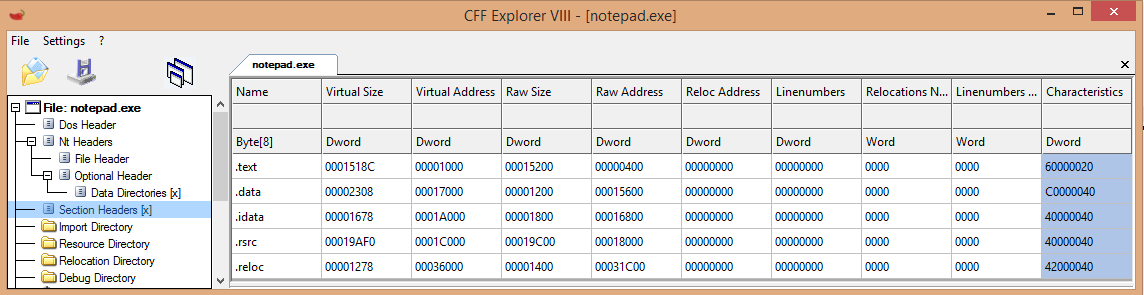
\includegraphics[scale=0.5]{Figures/pic6.PNG}
\caption{ La table des sections d'un fichier PE avec CFF Explorer.}
\label{fig :pic6} 
\end{center}
\end{figure}


le tableau~\ref{tab3} explique les champs qui sont vraiment intéressants : 
\begin{table}[H]
\begin{tabular}{|p{4.5cm}|p{10.5cm}|}
\hline \textbf{champ} &  \textbf{contenu}\\
\hline Name & Ce champ contient le nom de la section, il est là seulement à titre informatif pour le programmeur.\\
\hline VirtualAddress &	La RVA de la section. Le PE Loader vérifie et utilise la valeur de ce champ lorsqu'il place une section en mémoire.\\
\hline SizeOfRawData & La taille des données de la section, arrondie au prochain multiple de FileAlignment. Le PE Loader vérifie ce champ pour savoir combien d'octets de la section il va devoir placer en mémoire.\\
\hline PointerToRawData & L'offset fichier du début de la section. Le PE Loader utilise la valeur de ce champ pour trouver les données de la section dans le fichier.\\
\hline Characteristics & Contient des drapeaux indiquant par exemple si la section contient du code exécutable, des données non initialisées, si elle dispose d'un accès en écriture ou en lecture.\\
\hline
\end{tabular}
\caption{La structure de Table des Sections}
\label{tab3}
\end{table}


Chaque fichier PE contient un ensemble de sections, définit dans la Table des Sections. Une section est en fait un "segment" du fichier, possédant certaines particularités. Ci-dessous, Le tableau~\ref{tab4} montre
les différentes sections existantes.
\begin{table}[H]
\begin{tabular}{|p{2 cm}|p{12 cm}|}
\hline \textbf{Nom} &  \textbf{Description}\\
\hline .text & Généralement le code (instructions) du programmme.\\
\hline .bss & Contient des données non-initialisées.\\
\hline .reloc & Relocation.\\
\hline .data & Contient des données initialisées.\\
\hline .rsrc & Généralement les ressources du fichier (Curseurs, Sons, Menus ...)\\
\hline .rdata & Contient l'IAT d'un fichier.\\
\hline .idata & Contient l'IAT d'un fichier.\\
\hline .upx & Signe d'une compression UPX, propre au logiciel UPX.\\
\hline .aspack & Signe d'un package ASPACK, propre au logiciel ASPACK.\\
\hline .adata & Signe d'un package ASPACK, propre au logiciel ASPACK.\\
\hline
\end{tabular}
\caption{ Sections des fichiers PE}
\label{tab4}
\end{table}
La figure~\ref{fig :pic5} montre la table des sections d'un fichier PE avec éditeur hexadécimal :
\begin{figure}[H]
\begin{center}
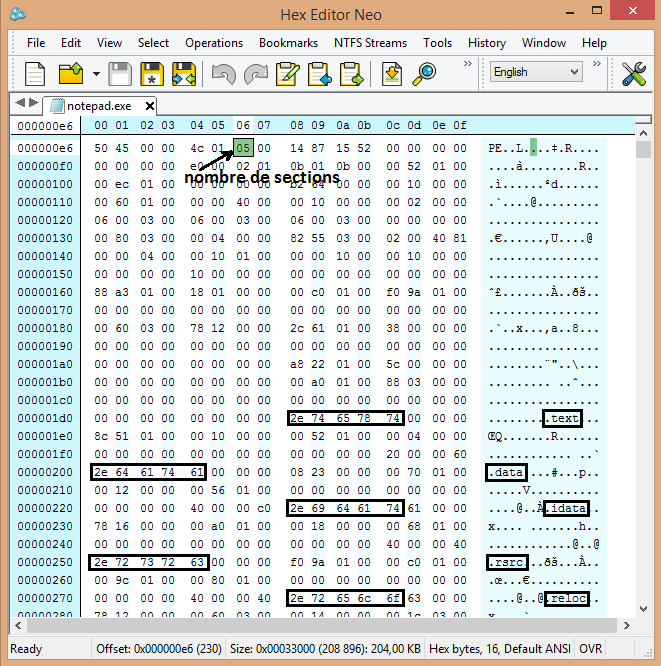
\includegraphics[scale=0.8]{Figures/pic5.PNG}
\caption{ La table des sections d'un fichier PE avec Hex Editor.}
\label{fig :pic5} 
\end{center}
\end{figure} 
\subsection{La table d'importation}
L'IAT, qui signifie \textbf{Import Address Table}, est une section (.idata ou .rdata) contenant les adresses des API importées par un logiciel, ainsi que les noms des DLL exportant ces fonctions. Les API, exportées par ces DLL, permettent aux logiciels de fonctionner correctement. Son existence est dû au fait que les API sont adressées différemment en fonction des OS.\\
La section \textbf{.idata} (ou \textbf{.rdata} parfois), qui contient cette IAT, est formaté d'une certaine façon. Il faut savoir en premier lieu qu'une structure nommée "ImageImportDescriptor" est utilisé pour chaque DLL appelée; plus une dernière de 5 DWORD mise à zéro qui définit une terminaison.\\
Pour chaque DLL importée, une structure nommée IMAGE\_THUNK\_DATA sera utilisée pour chaque API de cette
DLL; il y aura donc autant de IMAGE\_THUNK\_DATA que de fonctions exportées par une DLL, plus un dernier
DWORD spécifiant la terminaison de cette DLL. Une troisième structure, IMAGE\_IMPORT\_BY\_NAME, définit le nom des API ainsi que leur numéro ORDINAL (Nombre de 16 bits identifiant une fonction au sein d'une DLL). Il en existe autant qu'il y a d'API importées par DLL.
Par exemple, sur l'image~\ref{fig :IAT} d'exemple ci-dessous, il y a trois IMAGE\_IMPORT\_BY\_NAME définis pour user32.dll, car seulement trois de ses API sont utilisées par le programme.
\begin{figure}[H]
\begin{center}
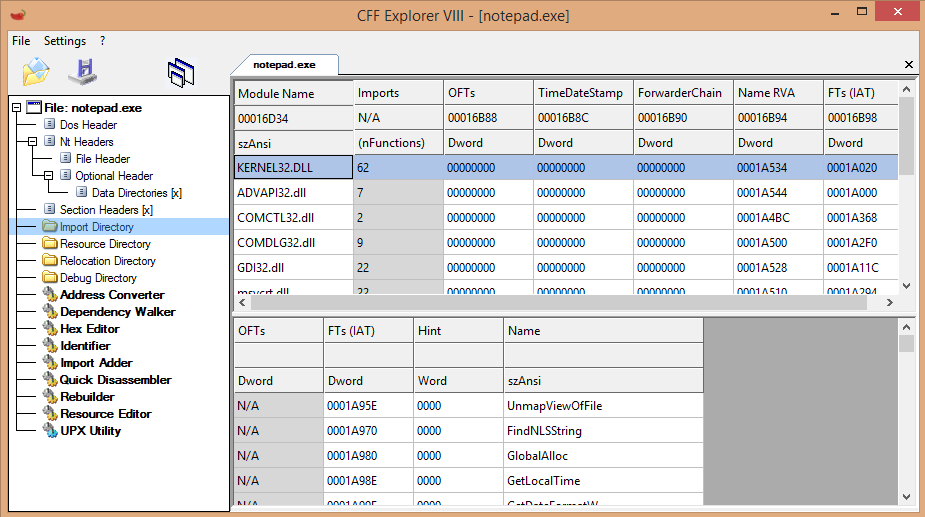
\includegraphics[scale=0.6]{Figures/pic7.PNG}
\caption{Table d'importation d'un fichier PE}
\label{fig :IAT} 
\end{center}
\end{figure}
La Table d'importation est prototypée comme suit :
\begin{lstlisting}

typedef struct _IMAGE_IMPORT_DESCRIPTOR {

DWORD Characteristics; 
DWORD OriginalFirstThunk; 
DWORD TimeDateStamp; 
DWORD ForwarderChain; 
DWORD Name; 
DWORD FirstThunk; 

} IMAGE_IMPORT_DESCRIPTOR;

typedef struct _IMAGE_IMPORT_BY_NAME {

WORD Hint; //Ordinal Number
BYTE Name[1]; //Name of function

} IMAGE_IMPORT_BY_NAME, *PIMAGE_IMPORT_BY_NAME;

typedef struct _IMAGE_THUNK_DATA {

PDWORD Function;
PIMAGE_IMPORT_BY_NAME AddressOfData;

} IMAGE_THUNK_DATA, *PIMAGE_THUNK_DATA;
\end{lstlisting}
\subsection{La table d'exportation}
Quand le PE Loader exécute un programme, il charge les DLL associées dans l'espace d'adressage du processus. Il extrait ensuite les informations des fonctions importées à partir du programme principal. Il utilise ces informations pour rechercher les adresses de ces fonctions dans les DLL, afin de les renseigner dans le code du processus. L'endroit où le PE Loader cherchera ces adresses se trouve être la table d'exportation de ces mêmes DLL.\\
Il existe deux manières pour une DLL ou un EXE d'exporter une fonction afin de la rendre utilisable par un programme externe : elle peut être exportée par nom, ou uniquement par ordinal.\\
Comme pour la table d'importation, la localisation de la table d'exportation peut être retrouvée dans le data directory. Ici, la table d'exportation en est le premier membre. La structure d'exportation est appelée IMAGE\_EXPORT\_DIRECTORY. Elle est prototypée comme suit :
\begin{lstlisting}
typedef struct _IMAGE_EXPORT_DIRECTORY {

DWORD  Characteristics;           /* 0x00 */
DWORD  TimeDateStamp;             /* 0x04 */
WORD   MajorVersion;              /* 0x08 */
WORD   MinorVersion;              /* 0x0a */
DWORD  Name;                      /* 0x0c */
DWORD  Base;                      /* 0x10 */
DWORD  NumberOfFunctions;         /* 0x14 */
DWORD  NumberOfNames;             /* 0x18 */
DWORD  AddressOfFunctions;        // 0x1c RVA from base of image
DWORD  AddressOfNames;            // 0x20 RVA from base of image
DWORD  AddressOfNameOrdinals;     // 0x24 RVA from base of image

} IMAGE_EXPORT_DIRECTORY, *PIMAGE_EXPORT_DIRECTORY;
\end{lstlisting}
\section{Le PE Loader}
Le PE Loader est un élément de Microsoft Windows permettant de reconnaître et de charger en mémoire des fichiers PE. C'est grâce à lui que Microsoft Windows peut exécuter les instructions d'un tel fichier.\\


Voici son fonctionnement global :
\begin{itemize}
\item Le PE Loader examine l'en-tête MZ-DOS afin de trouver l'offset de l'en-tête PE. S'il le trouve il saute dessus
\item Il vérifie la validité de l'en-tête PE. Si tel est le cas il saute à la fin de cet en-tête
\item Il lit les informations concernant les sections puis mappe ces sections en mémoire en employant un procédé de "File Mapping" (copie d'un fichier en mémoire).

\end{itemize}
        
\section{Les Packers}
Un Packer est un utilitaire dont le but est de compresser un programme afin de réduire sa taille initiale, tout en conservant son aspect exécutable ( le code original est retrouvé en mémoire lors de l'extraction ).\\
Néanmoins, avec le temps, des nouveaux packers sont apparus et ces derniers possèdent également la capacité de chiffrer le code du programme cible, ce qui aura pour effet de réduire son poids certes, mais qui de plus, va modifier son code d'exécution. Un algorithme des plus connu, et un des plus simple à contourner (clé généralement en dur dans le programme), est sans nul doute XOR (OU-Exclusif).\\
Bien entendu, la partie "déchiffrement" effectué lors du lancement du programme packé/chiffré sera établie de manière transparente pour l'utilisateur. Mais un désassembleur  verra cela autrement, en visualisant un code (très) différent de la normale.\\

Les cybercriminels ont recours aux packers pour eviter que l'antivirus puisse identifier le malware rapidement. le meme malware (même identifié par l'antivirus) lorsqu'il est packé, la signature ne matchera pas et il ne sera pas détecté. mais comme les antivirus ont du mal a analyser les malwares en mémoire (lorsqu'ils sont dépackés), alors les packers sont une bonne protection pour les cybercriminels. Aussi, ils servent à ralentir les analystes dans l'analyse de malware car ils intégrant des méthodes d'antidebug, antivm, et autres.
un packer malveillant peut identifier qu'il est exécuté dans une virtuel machine, qu'il est analysé avec un debugger, ...\\

Il existe de nombreux packers tel que : Armadillo, ASPack \& ASProtect, NeoLite, PKLite, Petite v1.4/2.x, PolyCrypt PE, Shrinker, VBox, WWPack(32), ...\\

Un des Packers sans nul doute le plus connu est UPX, qui s'occupe de réduire la taille d'un exécutable de manière très efficace (près de 50\%). La figure~\ref{fig :UPX} montre le packer UPX.
\begin{figure}[H]
\begin{center}
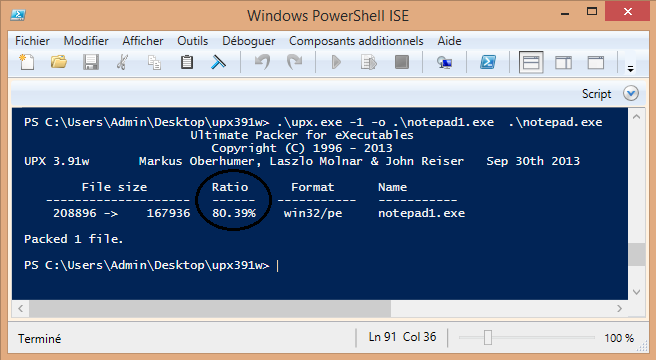
\includegraphics[scale=0.7]{Figures/UPX.png}
\caption{Le Packer UPX}
\label{fig :UPX} 
\end{center}
\end{figure}
Lorsque le programme packé est exécuté, un chargeur/décompresseur (wrapper program) est exécuté aussi pour décompresser le fichier packé puis exécuter le fichier décompressé, comme le montre la figure~\ref{fig :PACK}. Quand un  programme packé est analysé statiquement, seul le chargeur/décompresseur peut être disséqué~\cite{ANA}.
\begin{figure}[H]
\begin{center}
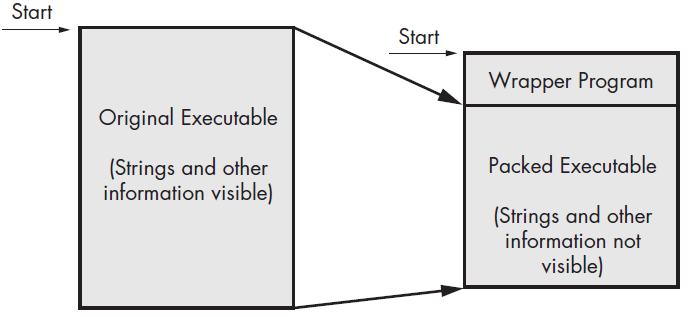
\includegraphics[scale=0.6]{Figures/PACK.png}
\caption{Fichier original et fichier packé}
\label{fig :PACK} 
\end{center}
\end{figure}
\subsection{Détection des Packers avec PEiD}
Une façon de détecter des fichiers compressés (packés) est avec le programme PEiD. Il est possible d'utiliser PEiD pour détecter le type de packer ou le compilateur utilisé pour construire une application, ce qui rend l'identification d'un fichier packé, avec un packer connu, beaucoup plus facile.\\
PEiD contient une base de signature permettant d'identifier les packers/compilateurs utilisés, cette base s'appelle UpdateDB.txt.
 La figure~\ref{fig :PEID} montre l'analyse d'un fichier .exe par PEiD.
\begin{figure}[H]
\begin{center}
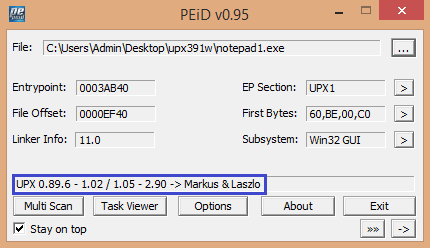
\includegraphics[scale=0.9]{Figures/PEID.PNG}
\caption{Le programme PEiD}
\label{fig :PEID} 
\end{center}
\end{figure}
On remarque que PEiD a identifié le fichier comme étant packé avec UPX Version 0.89.6-1.02 ou de 1.05 à 2.90.
\newpage
\section{Conclusion}
Le format PE (Portable Executable, exécutable portable) est le format des fichiers exécutables et bibliothèques pour les systèmes d'exploitation Microsoft Windows : .exe (programmes), .ocx (OLE et ActiveX), .dll et .cpl (élément du panneau de configuration Windows). C'est un format dérivé du COFF.\\


Un fichier exécutable PE est structuré d'en- MZ-DOS, segment DOS, en-tête PE et la table des sections. Le PE Loader est un élément de Microsoft Windows permettant de reconnaître et de charger en mémoire des fichiers PE. \\
Un Packer est un utilitaire dont le but est de compresser un programme afin de réduire sa taille initiale, tout en conservant son aspect exécutable.\\

Dans le chapitre suivant, on va présenter une conception de notre antivirus ainsi la conception de parseur de PE.

\chapter{Conception de l'antivirus}
\section{Introduction}
Un antivirus est un logiciel de protection dont le but est de détecter les malwares (comme par exemple les virus, vers, chevaux de Troie, ...). Pour cela, il inspecte la mémoire, les disques durs de l'ordinateur et les volumes amovibles (CD, DVD, clé USB, disque dur externe...) pour vérifier que les fichiers qui y sont présents ne contiennent pas de codes malveillants connus. Il permet aussi d'effectuer régulièrement des analyses planifiées.\\

Un antivirus protège contre les codes malveillants qu'il connaît ou qu'il reconnaît. Le temps que l'éditeur écrive la signature d’un nouveau malware et que l'antivirus la télécharge, l'internaute n'est pas protégé.\\

Dans ce chapitre, nous présentons les différentes phases suivies pour la conception  de l'antivirus.

\section{Conception de l'antivirus} 
Après avoir cité les phases de cycle de vie d'un malware (section 1.3.3, chapitre 1), nous constatons que les éditeurs des antivirus ne peuvent pas intervenir durant les deux phases "infection" et "maladie", contrairement à la phase d'incubation.\\

Donc l'antivirus sera composé de deux outils essentiels. Un outil qui analyse les fichiers PE (parseur de PE)  et un  scanneur de malwares.\\

Le diagramme des cas d'utilisation suivant donne une vision globale du comportement fonctionnel de l'antivirus.
\begin{figure}[H]
\begin{center}
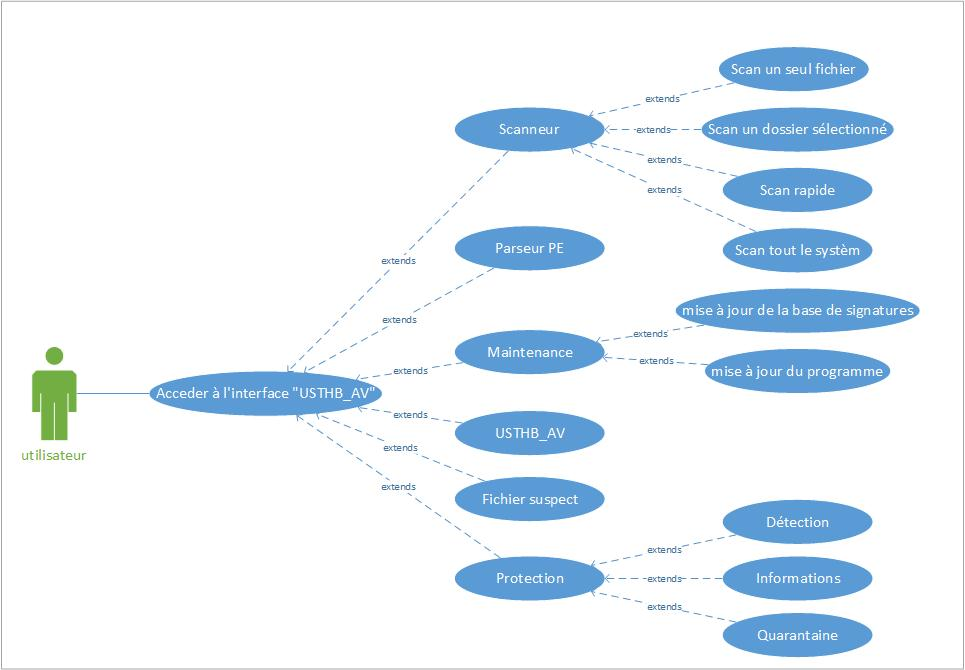
\includegraphics[scale=0.6]{Figures/antivirus.jpg}
\caption{Diagramme des cas d'utilisation de l'antivirus.}
\label{fig :mise} 
\end{center}
\end{figure}
\subsection{Parseur de PE}
\subsubsection{Objectif du parseur }
L'objectif de ce travail est d'observer le contenu d'un fichier exécutable. Avec ce parseur nous pouvons visualiser et examiner les fichiers de format PE ainsi que leurs structures internes (voire chapitre 2).\\


Le parseur PE sert à analyser les fichiers PE et d'autres usages différents. Il comporte un analyseur d'entête PE, une visionneuse des fonctions API importées, un testeur de validité du format PE, vérificateur et détecteur des packers.
\subsubsection{Vérifier  la validité d'un fichier PE}
Le test de validité d'un fichier de format PE, se fait selon les  étapes suivantes :
\begin{itemize}
\item Vérifier que le fichier a un entête DOS-MZ valide en comparant le premier WORD du fichier avec la valeur IMAGE\_DOS\_SIGNATURE qui doit être égale à "MZ";
\item Si le fichier a un entête DOS valide, on utilise la valeur contenue dans le champs \_lfanew pour trouver l'entête PE;
\item Comparer le premier DWORD de l'entête PE avec la valeur IMAGE\_NT\_SIGNATURE qui doit être égale à "PE00". Si les deux valeurs concordent, alors on peut considérer le fichier comme un fichier potentiellement valide.
\end{itemize}
L'organigramme suivant montre le test de validité d'un fichier PE :
\begin{figure}[H]
\begin{center}
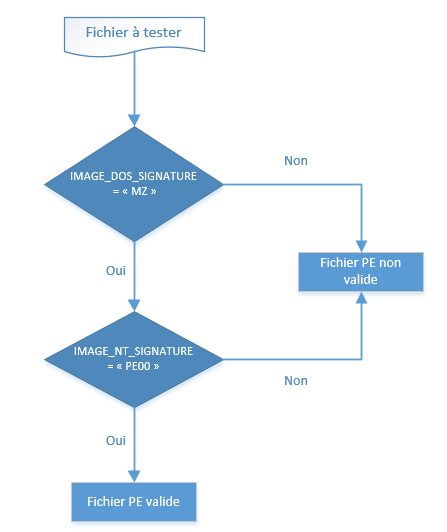
\includegraphics[scale=0.6]{Figures/org.PNG}
\caption{Test de validité d'un fichier PE.}
\label{fig :org} 
\end{center}
\end{figure} 
\subsubsection{Visualiser le contenu d'un fichier PE}
Dans cette étape nous affichons les informations internes du fichier PE, le nombre de sections, ses détails et quelques caractéristiques de ce dernier.
\begin{itemize}
\item Entry point : récupérer l'adresse mémoire où  sera chargé le fichier PE;
\item Détail PE   : afficher les caractéristiques du fichier PE et toutes les informations nécessaires pour charger ce  fichier en mémoire (citées dans la section 2.3.4 et  2.3.5 , chapitre 2);
\item Les sections PE : afficher les sections du fichier PE et leurs détails (cités dans la section 2.3.6 de chapitre 2).
\end{itemize}
\subsubsection{La table d'importation}
Afficher les DLL importées par le fichier PE après avoir chargé en mémoire, lister, pour chaque DLL, les fonctions utilisées (voir la section  2.3.7 et 2.3.8, chapitre 2).
\subsubsection{Détection des packers}
Enfin, nous examinons si le fichier PE est pacqué (voir la section 2.4 de chapitre 2 )  ou non, en utilisant une liste noire :
\begin{itemize}
\item La détection se fera au moyen d'un test de l'existence des noms de sections de fichier PE dans une liste noire des fonctions, les plus utilisées dans la compression. Si la fonction existe dans la liste, le fichier est conséquemment pacqué avec cette dernière, \end{itemize}
\subsection{Scanneur de malwares }
\subsubsection{Objectifs}
L'objectif de l'antivirus est tacitement de détecter les malwares avant leur exécution en mémoire, rechercher sur disque dur toute indication des malware; l'antivirus fonctionne en mode statique (voir la section 1.4.2.1, chapitre 1).
\subsubsection{Mécanismes de détection }
Pour atteindre cet objectif, nous devons étudier  les techniques anti-virales utilisées dans le mode de fonctionnement statique, recherche par signature, analyse spectrale et le contrôle d'intégrité (voir la section 1.4.3, chapitre 1). Le tableau~\ref{comp} montre une comparaison entre ces trois techniques :
\begin{table}[H]
\begin{tabular}{|p{4.5cm}|p{5cm}|p{5cm}|}
\hline \textbf{Technique} &  \textbf{Avantages} & \textbf{Inconvénients}\\
\hline \textbf{Recherche par signature} & détecter les malwares avant leurs exécutions en
mémoire & n'est pas capable de détecter les nouveaux malwares\\
\hline \textbf{Analyse spectral} & permet de détecter des nouveaux malwares & génère trop de faux positif \\
\hline \textbf{Contrôle d'intégrité}& permet de détecter les modifications de fichiers sur le disque & génère trop de faux positif \\
\hline
\end{tabular}
\caption{Comparaison entre les techniques anti-virales}
\label{comp}
\end{table}


D'après cette comparaison nous préférons la  recherche par signature, car elle répond avantageusement et favorablement à notre objectif.
\subsection{Composants du moteur antivirus}
\subsubsection{Base de signatures}
La base de signatures référence des dizaines de milliers de malwares, elle doit être mise à jour fréquemment pour reconnaître les nouveaux programmes malveillants~\cite{viruslist}.\\

La base de données d'un antivirus est un conteneur servant à stocker  l'ensemble des  signatures de malwares reconnus par l'antivirus pour être une référence de scan, cette base de signatures a plusieurs caractéristiques : type de la base de données, type et format des signatures et la façon de sa mise à jour.
\subsubsection{Type de la base de données}
Nous pouvons extraire des données de diverses bases de données, comme Microsoft Office Access, Microsoft SQL Server, les services OLAP de Microsoft SQL Server, de classeurs Excel et de fichiers de texte.\\


D'après le type et le format des signatures de l'antivirus, qui est un format texte, notre base de signatures sera une base de données orientée texte.\\

Une base de données orientée texte (ou "Base de données dans un fichier plat", de l'anglais "Flat file database") est un modèle de base de données (qui se présente,généralement, sous forme d'une table) sous la forme d'un simple fichier (formats .txt, .ini ,...).\\


Un fichier plat est un fichier texte contenant généralement un seul enregistrement par ligne, cet enregistrement est la signature de malware, chaque ligne de ce fichier texte correspond à une signature.\\

Le choix des fichiers plats se fait à seule fin de stocker les signatures des malwares, on n'a pas fait recours à une base de données "sql" car il n'y a pas d'avantages réels en faveur de l'utilisation de celle-ci et comprend mêmement de façon certaine quelques désavantages. Pour les actions standards (visualiser, éditer, ...), conserver l'information dans des fichiers plats est clairement plus rapide que d'y accéder au moyen d'une base de données. Sachant que l'avantage est essentiellement basé sur la simplicité, facilité de déploiement, légèreté et la non nécessité de dépendre d'un SGBD.
\subsubsection{Type de signature }
La technique anti-virale utilisée par notre antivirus pour détecter les malwares est la détection par signature "scanning", qui peut s'exprimer sous plusieurs types tels que : hash de malware et suite hexadécimale, cette  dernière est récupérée depuis le code  binaire du malware.
\begin{itemize}
\item \textbf{Hash de fichier : }une fonction de hachage (parfois appelée fonction de condensation) est une fonction permettant d'obtenir un condensé (appelé aussi condensat ou haché ou en anglais message digest) d'un texte, c'est-à-dire une suite de caractères assez courte représentant le texte qu'il condense. La fonction de hachage doit être telle qu'elle associe un seul haché à un texte en clair (cela signifie que la moindre modification du document entraîne la modification de son haché). D'autre part, il doit s'agir d'une fonction à sens unique (one-way function) afin qu'il soit impossible de retrouver le message original à partir du condensé. S'il existe un moyen de retrouver le message en clair à partir du haché~\cite{hashage}.\\

Les algorithmes de hachage les plus utilisés actuellement sont :\\


\begin{list}{•}{}

\item \textbf{Hash MD5}(Message Digest) : Développé par Rivest en 1991, MD5 crée une empreinte digitale de 128 bits à partir d'un texte de taille arbitraire en le traitant par blocs de 512 bits. Il est courant de voir des documents en téléchargement sur Internet accompagnés d'un fichier MD5, il s'agit du condensé du document permettant de vérifier l'intégrité de ce dernier~\cite{sha}.\\

Exemple  pour md5 : \textbf{e1ade9d04ad99dd70ec25b83841d8b72}\\


\item \textbf{SHA}(Secure Hash Algorithm) : pouvant être traduit par Algorithme de hachage sécurisé, SHA crée des empreintes d'une longueur de 160 bits. SHA-256 est une version améliorée de SHA, SHA-256 devient en 2002 un standard fédéral de traitement de l'information (FIPS du NIST). Elle produit un hachage de 256 bits~\cite{sha}.\\
Exemple pour sha1 : \textbf{2fd4e1c67a2d28fced849ee1bb76e7391b93eb12}\\
\newpage
En 2004, une équipe chinoise a découvert des collisions complète "même résultat d'hachage pour deux fichier différant", md5 n'est donc plus considère comme sûr au sens cryptographie, et il est recommander d'utiliser la fonction sha256 qui est plus fiable pour notre signature~\cite{shamd}.\\


\end{list}
\item \textbf{Suite hexadécimale : }la signature est une suite hexadécimale récupérée depuis le code binaire de malware, d'une taille variable et un offset différent, il faut que le malware soit bien identifié par cette suite.  
\end{itemize}
\subsubsection{Choix du type de signature}
\textbf{Quel est le type le plus fiable et rapide pour le bon fonctionnement de l'antivirus ?}\\
Pour répondre à cette question, nous faisons une expérience par rapport aux points suivants : nombre de malwares détectés, temps de détection, faux positif et nombre de malwares polymorphes détectés, par rapport à une base du 7404 signatures, en plaçant 10 malwares dans un dossier qui contient 50 fichiers sains, et pour tester l'efficacité de détection des malwares polymorphes par les deux types de signature, nous ajoutons quatre malwares modifiés avec l'éditeur Hexadécimal HxD, en gardant toujours leur   fonctionnement, le volume de données analysées est de 4.2 G, à la fin de cette expérience nous avons obtenu les résultats indiqués dans le tableau~\ref{signatures} : 
\begin{table}[H]
\begin{center}
\begin{tabular}{|p{3cm}|p{2cm}|p{3cm}|p{2cm}|p{2cm}|}
\hline Type de signature &  malwares détectés & Temps de détection & Faux positifs & Malwares polymorphes\\
\hline Hashage de Fichier & 10 & 04:23:12:34 & 0 & 0 \\
\hline Suite hexadécimal & 15 & 00:01:34:01 & 1 & 4 \\
\hline
\end{tabular}
\caption{Comparaison entre les types de signatures}
\label{signatures}
\end{center}
\end{table}
\textbf{\textit{Analyse des résultats }}
\begin{itemize}
\item Hashage de fichier : dix malwares détectés, pas de faux positif et aucun malware polymorphe n'a été détecté dans un temps dépassant de quatre heures 
\item Suite hexadécimal : onze malwares détectés, un faux positif et quatre malwares polymorphes détectés dans un temps très court. \\


D'après les résultats obtenus, nous préférons utiliser la suite hexadécimale pour notre signature car elle nous permet de détecter tous les malwares "10 malware", ainsi que les malwares polymorphes, mais avec un seul Faux positif, dans un temps inférieur à ce de type hachage fichier qui ne nous permet pas à détecter les malwares polymorphes. 

\end{itemize}
\newpage
\subsubsection{Format de signatures}
Le format de signature est le suivant :\\
\begin{table}[H]
\begin{center}
\begin{tabular}{|p{3.5cm}|p{3.5cm}|p{3.5cm}|p{3.5cm}|}
\hline Offset & Suite hexadécimale &  Nom de malware & Type de malware \\
\hline
\end{tabular}
\caption{Format de signatures}
\label{signatures}
\end{center}
\end{table}

\begin{itemize}
\item \textbf{Offset : }l'offset d'où la suite hexadécimale a été récupéré  
\item \textbf{Suite hexadécimale : }une suite d'octets récupérés depuis le code du malware 
\item \textbf{Nom de malware : }nom de malware attribue par les éditeurs de l'antivirus 
\item \textbf{Type de malware : }virus, worm, cheval de troie, ...
\end{itemize} 
Ex : 58ab|38896E0E41B0CB35F3D7B94D6D973F143A75CD97F974A514869E1 : Conficker/Worm

\subsubsection{La mise à jour}
L'efficacité des solutions antivirus dépend des bases de signatures de définitions du malware. Ces bases sont dynamiques intrinsèquement,et ce, étant donné l'activité des auteurs de malware. Par exemple, les analystes viraux de Kaspersky Lab détectent et ajoutent cent nouvelles menaces, quotidiennement, à la base de l'antivirus~\cite{mise}.\\


Néanmoins, une mise à jour régulière de la protection antivirus est plus importante que jamais, étant donné la rapidité avec laquelle les menaces actuelles sont capables de se propager. Les éditeurs d'antivirus ont réduit l'intervalle entre les mises à jour de signatures de façon trimestrielle à une façon mensuellement et finalement à une façon quotidienne.\\


Désormais, Kaspersky Lab fournit les mises à jour de définitions virus toutes les heures.
Et pour cela, nous proposons pour notre antivirus deux méthodes pour le mettre à jour, l'une est \textbf{automatique} et l'autre \textbf{manuelle} déclenchée de la part de l'utilisateur.\\


Dans les deux cas, la mise à jour sera effectuée selon les étapes suivantes :

\begin{itemize}
\item Télécharger un fichier nommé "info.txt" depuis "Github"
\item Récupérer un hash de la base de signatures de site web depuis ce fichier téléchargé 
\item Comparaison entre le hash récupéré de fichier "info.txt" et le hash de la base de signatures actuel, si les deux hash sont identiques alors l'antivirus informe l'utilisateur que sa base virale est à jour, sinon nous effectuons les tâches suivantes:
\begin{list}{•}{}
\item Télécharger un fichier texte depuis le site de l'antivirus nommé "new\_bdd\_mal.txt" 
\item Remplacer l'ancienne base de signatures par la nouvelle 
\item Informer l'utilisateur que la mise à jour est bien terminée.

\end{list}

\end{itemize}

Le diagramme suivant montre les étapes pour faire la mise à jour de notre antivirus :
\begin{figure}[H]
\begin{center}
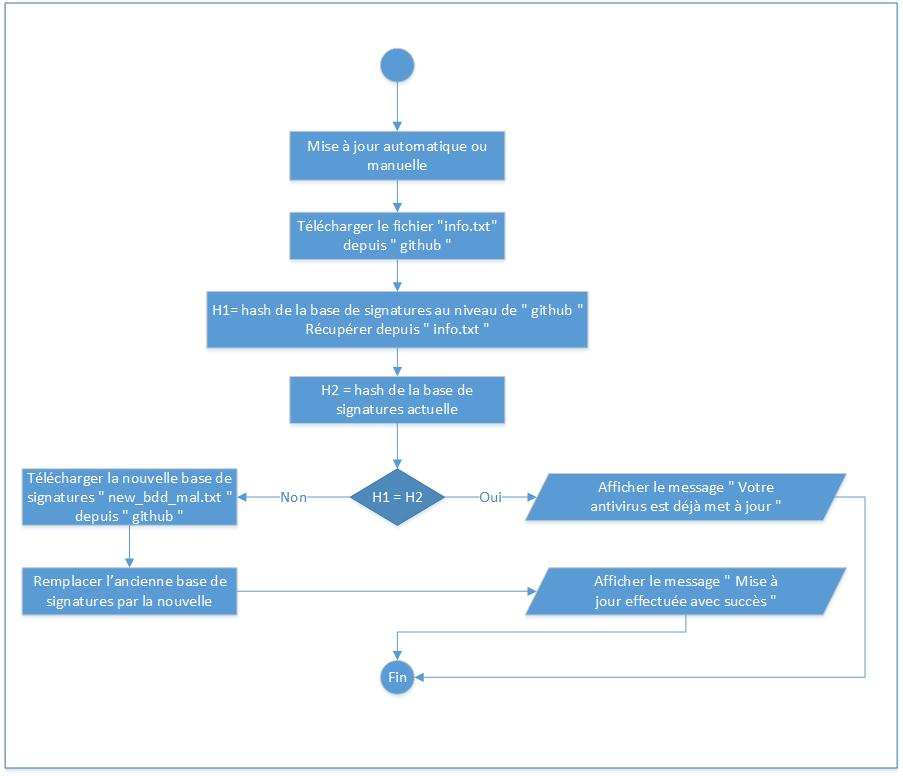
\includegraphics[scale=0.6]{Figures/mise.jpg}
\caption{Les étapes de la mise à jour de l'antivirus.}
\label{fig :scan} 
\end{center}
\end{figure}


\subsubsection{Les types de scan} 
L'antivirus examine (scan) le système à la demande : un fichier, un dossier ou tous les fichiers du disque. Un scan complet consomme beaucoup de ressources matérielles et du temps, mais il est conseillé de le faire de temps en temps.\\


Dans cette partie, nous allons proposer quatre manières pour effectuer un scan :\\

\begin{itemize}
\item Scan un seul fichier : il effectue une analyse d'un seul fichier sélectionné  
\item Scan un dossier sélectionné : il effectue une analyse d'un répertoire  sélectionné  
\item Scan rapide : il effectue uniquement une analyse rapide du disque system "C:\ de l'ordinateur", seulement les fichiers aux extensions perceptibles à une infection (.exe, .ocx, .dll, .cpl) seront testés
\item Scan tout le système : il effectue un scan de tous les disques de l'ordinateur.

\end{itemize}
\subsubsection{La présentation des résultats d'analyse}
Après avoir effectué un scan selon l'un des types cités précédemment, les résultats de scan seront présentés à l'utilisateur dans une grille, pour chaque type de scan, le rapport comportera les champs suivant :
\begin{itemize}

\item Nom du malware : un nom attribué par les éditeurs des malwares
\item Type : c'est le type de malware (section 1.3.2, chapitre 1)
\item Chemin : le chemin courant du malware détecté.  

\end{itemize}
\subsection{Autres fonctionnalités }
\begin{itemize}
 
\item La langue d'utilisation : dans cette option, nous offrons à l'utilisateur la possibilité de choisir la langue,  nous  proposons  deux langues : Anglais et Français 
\item Information sur la protection : cette fonctionnalité permet à l'utilisateur de visualiser  des informations concernant l'état actuel de l'antivirus comme :
\begin{list}{•}{}
\item La liste des malwares détectés  par notre antivirus classés par leur nom et type 
\item Informations sur la base de signatures telles que sa taille "nombre de signatures", le nombre des virus et la version actuelle de l'antivirus
\item Quarantaine : cette fonctionnalité permet d'accéder au dossier quarantaine, visualiser son contenu.
\end{list}

\item L'accès au site officiel de l'antivirus : permet à l'utilisateur de découvrir les fonctionnalités de l'antivirus, et les éventuels problèmes pouvant être rencontrés durant l'utilisation, télécharger le guide d'utilisation et actualités concernant la sécurité informatique et bien évidemment, soumettre des questions.
\item Guide d'utilisation : un guide pratique expliquant la manière d'utilisation de l'antivirus et toutes ses tâches
\item Mise à jour de programme : effectuera selon les mêmes étapes de la mise à jour de la base de signatures virales, au lieu de télécharger la base de signatures, des fichiers ".dll" seront téléchargés
\item L'envoi d'un fichier suspect : permet à l'utilisateur d'envoyer un fichier suspect compressé, protégé par le mot de passe "infected" à l'équipe d'analyse de l'antivirus.
\end{itemize}
\section{La façon de présenter l'antivirus}
L'antivirus sera présenté au moyen d'une interface graphique, qui permettra de visualiser l'état actuel de la protection, modifier la langue, effectuer manuellement un scan et d'utiliser l'outil parseur PE pour avoir des détails techniques concernant un fichier PE, l'accès à cette interface peut se faire selon trois manières différentes :
\begin{itemize}
\item A partir d'un raccourci, qui permet d'appeler l'interface de l'antivirus
\item A partir de l'icône de l'antivirus présentée dans la zone de notification "systray", en bas à droite de l'écran près de l'horloge par un simple clic
\item A partir du menu Démarrer, par un clic sur Programmes suivi par la sélection du nom d'antivirus. \\
\end{itemize}
L'antivirus se lance automatiquement au démarrage de Microsoft Windows.
\section{Fonctionnement de  l'antivirus :}
D'après cette conception, notre antivirus a deux tâches essentielles et primordiales, un parseur PE est un outil de scan
\subsection{Parseur PE }
L'utilisateur sélectionne un fichier depuis le système ou les disques amovibles pour afficher ses détails techniques, par un simple clic sur un bouton appelé "Parseur PE" qui permet d'accéder à une nouvelle page et un nouveau bouton " ... ", ce dernier permet d'accéder aux différents disques de votre système pour choisir un fichier par un clic sur le nom de fichier sélectionné, suivi d'une validation du choix avec le bouton "OK", les résultats de l'analyse seront affichés dans une fenêtre graphique, ainsi que le chemin de fichier sélectionné.
\subsection{Scanneur de malwares}
\subsubsection{phase de scan}
L'utilisateur sélectionne un type de scan, à savoir; scan rapide, scan d'un seul fichier, scan d'un dossier sélectionné ou un scan de tout le système, ensuite l'antivirus analysera  les fichiers relatifs au scan sélectionné, et ce, comme suit :\\

\begin{itemize}
\item Parcourir la base de signatures, pour chaque signature, nous testons leur apparence dans le code binaire de fichier testé selon les étapes suivantes : \\
\begin{list}{•}{}
\item Récupérer un offset depuis la signature testée
\item Récupérer la suite hexadécimale relative a l'offset récupéré, depuis le code binaire du fichier testé
\item Comparer la suite de la signature testé avec la suite récupérée.
\end{list}
\item Si les deux suites comparées sont identiques, nous sommes devant deux versions :
\begin{list}{•}{}
\item Scan d'un seul fichier : le fichier est signalé comme malware, et c'est la fin de scan
\item Autre type de scan : le fichier est signalé comme malware, ce qui nécessite la ré-exécution des étapes de scan dès le début pour le fichier suivant.
\end{list}
\item Si les deux suites comparées sont différents, nous testons la signature qui suit et ainsi de suite, à la fin de cette opération, si aucune signature n'a été trouvée; on est devant deux cas :
\begin{list}{•}{}
\item Scan d'un seul fichier : fin de scan
\item Autre type de scan : ce qui nécessite de refaire les étapes de scan dès le début pour le fichier suivant.\\
\end{list}
\end{itemize}

Le diagramme suivant montre les étapes de scan:
\begin{figure}[H]
\begin{center}
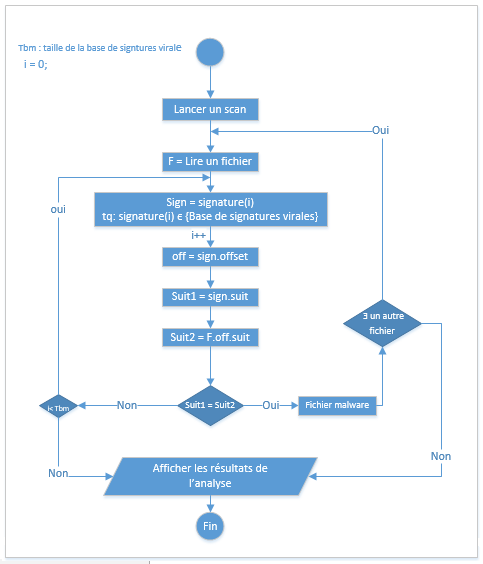
\includegraphics[scale=1]{Figures/scans.jpg}
\caption{Diagramme des étapes de scan.}
\label{fig :mise} 
\end{center}
\end{figure}
\subsubsection{Traitement des résultats de scan }

Après la détection d'un malware, nous proposons les actions suivantes :
\begin{itemize}
\item \textbf{Supprimer : }permet de supprimer le fichier signalé comme malware depuis son emplacement d'origine;  
\item \textbf{Mettre en Quarantaine : }si le fichier signalé ne peut ou ne doit pas être supprimé (fichier sensible, document personnel) alors il sera isolé jusqu'à une éventuelle opération, l'isolation se fait dans un dossier nommé  "quarantaine" 
\item \textbf{Ne rien faire : }Si aucune action n'est souhaitable, le fichier est ignoré.\\
\end{itemize} 
\section{Gestion de la base de signatures virales}
La détection d'un nouveau malware se fera par les éditeurs d'antivirus ou par un signalement (l'utilisateur envoie le malware compressé avec le mot de passe de décompression) de la part des utilisateurs, une fois détecté le malware sera analysé pour identifier son nom, son type,  son fonctionnement et son objectif.\\

    
Après la phase d'analyse, nous allons attribuer une signature de détection à ce malware, qui lui est propre, la génération de la signature virale commence par la récupération  de la suite hexadécimale qui identifie de manière unique le malware, suivie par l'association de l'offset, nom et du type de malware à cette suite.\\


Pour chaque nouveau malware détecté, nous devons mettre à jour la base de signatures virales, cette mise à jour  comporte plusieurs tâches qui sont gérées uniquement par les administrateurs d'antivirus, ces tâches sont :
\begin{itemize}

\item \textbf{Ajouter une signature : }permet à l'administrateur d'ajouter une nouvelle  signature à la base de signatures, l'ajout d'une signature se fait selon les étapes suivantes :
\begin{list}{•}{}
\item Sélectionner le malware à signer
\item Choisir l'offset de la suite hexadécimale à l'aide de parseur PE, l'offset peut être la valeur de l'EntryPoint ou l'offset de l'un des sections ".data", ".code", ...
\item Récupérer la suite relative à l'offset choisi
\item Tester l'apparence de cette suite dans la base de fichiers légitimes afin d'éviter les faux positifs pour la signature générée
\item Associer le nom et le type de malware qui ont été définis par l'analyste à la suite et l'offset généré. La génération d'une suite est terminée par l'insertion de cette dernière dans la base de signatures virale.\\ 
\end{list}
La figure~\ref{fig :generation} montre les étapes à suivre pour générer des signatures :
\begin{figure}[H]
\begin{center}
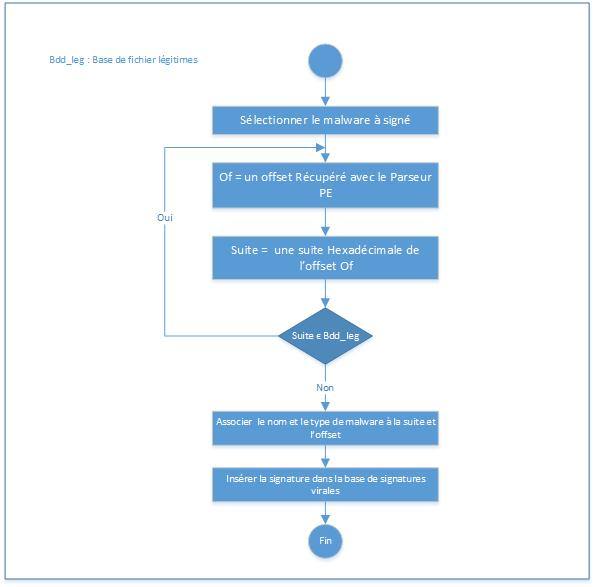
\includegraphics[scale=0.7]{Figures/generation.jpg}
\caption{Les étapes de génération d'une signature.}
\label{fig :generation} 
\end{center}
\end{figure}

\item \textbf{Afficher la base de signatures : }permet d'afficher le contenu de la base de signatures 
\item \textbf{Afficher la base de malwares : }permet de lister les noms de malwares
\item \textbf{Supprimer une signature : }supprime une signature identifiée par le nom de malware
\item \textbf{générer le fichier "info.txt" : } après chaque mise à jour, l'administrateur doit générer le fichier "info.txt" pour le charger sur GitHub. 
\end{itemize}


\section{Les faux positifs }
Pour éviter ou minimiser les faux positifs, nous allons construire une base de données des fichiers légitimes, qui présentent les fichiers fondamentaux d'une installation Microsoft Windows fraiche.\\

Et pour chaque signature virale générée, nous allons tester son apparence dans cette base des fichiers légitimes, si cette dernière existe, nous devons régénérer une autre signature, et ce, jusqu'à l'arrivée d'une signature qui n'existe plus. 

\subsection{Description de la base de fichiers légitimes}
La base des fichiers légitimes, comporte les fichiers déclarés par les éditeurs d'antivirus comme fichiers légitimes. Pour bien vérifier l'intégrité d'un fichier, nous utilisons la fonction d'hachage sha256, donc le fichier légitime sera stocké par son hash dans un fichier plat.
\subsection{Gestion de la base de fichiers légitimes}
Pour chaque nouveau fichier qui fait partie d'une nouvelle version Microsoft Windows ou mise à jour.l'administrateur met à jour la base de fichiers légitimes par l'insertion de ce fichier dans cette dernière, attribuer un nom au fichier qui est le hash de ce dernier .\\

Le diagramme de cas d'utilisation suivant donne une vision globale sur les tâches effectuées par l'administrateur d'antivirus.
\begin{figure}[H]
\begin{center}
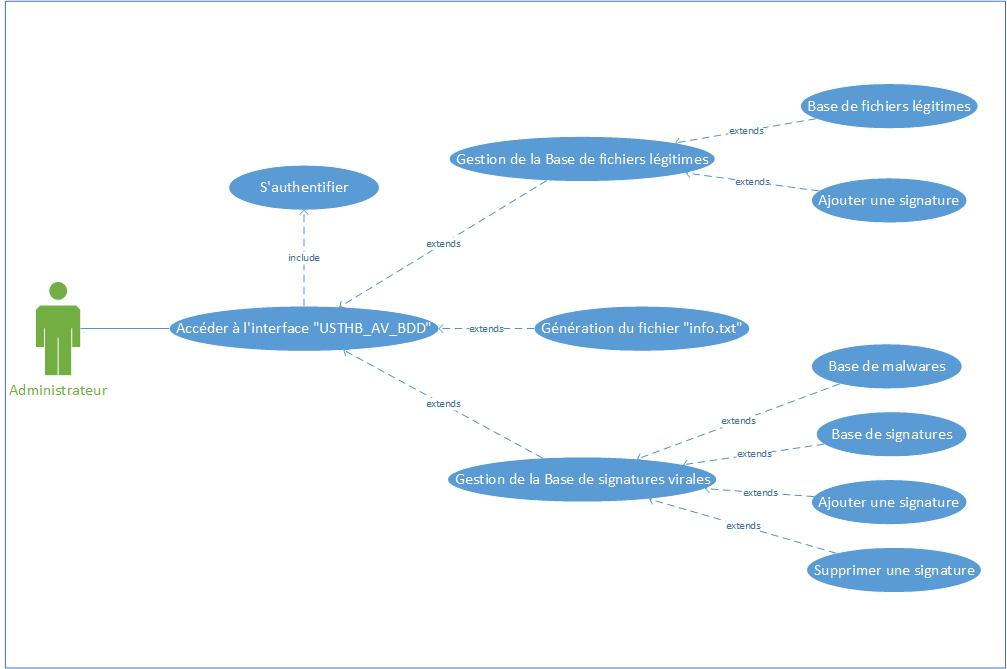
\includegraphics[scale=0.6]{Figures/Admin.jpg}
\caption{Détail de la gestion de la base de signatures.}
\label{fig :mise} 
\end{center}
\end{figure}

\section{Conclusion}
Dans ce chapitre, nous avons détaillé la conception de l'antivirus  qui est composée de deux outils, \textbf{un parseur PE} et \textbf{un Scanneur de malwares}.\\

Le parseur PE permet de visualiser les informations techniques d'un fichier PE et pour le scanneur, nous avons adopté la technique anti-virale de recherche par signature de type suite Hexadécimale, et pour éviter les faux positifs nous avons proposé une base de  signatures des fichiers légitimes.\\

 
Dans le chapitre suivant, l'implémentation de la solution anti-virale sera abordée.
\chapter{Implémentation}
\section{Introduction}

L'implémentation d'un projet consiste à réaliser au mieux les fonctionnalités décrites au niveau de la conception.\\

Dans ce qui suit, nous présentons l'environnement de développement, les fonctionnalités générales du l'antivirus ainsi que des captures d'écran illustrant cela.


\section{Outils utilisés}
\subsection{L'environnement de développement (Visual Studio) }
Pour implémenter notre antivirus nous avons opté pour l'utilisation de Microsoft Visual Studio comme un environnement de développement.
\subsection{Visual Studio}
Microsoft Visual Studio est un ensemble complet d'outils et de services destinés pour aider à créer des applications très variées, et pas seulement pour la plateforme Microsoft. Visual Studio connecte également l'ensemble de projets, équipes et parties prenantes. Désormais, les développeurs peut travailler avec une plus grande agilité de presque n'importe où, quel que soit l'outil de développement utilisé (par exemple: Eclipse ou Xcode). 
\subsection{Langages du Visual Studio}
Visual studio est un environnement polyvalent très riche en termes de langage de programmation permettant aux développeurs de créer toute une gamme d'applications, il comporte 05 langages de programmations : Visual C++, Visual C\#, Visual Basic, Visual F\#, JavaScript. 
\subsection{Langage de programmation C\# }
Dans l'implémentation de notre antivirus, nous avons utilisé le langage C\#. Visual C\# est un langage de programmation multi paradigme moderne et généraliste qui permet de créer des applications à l'aide de Visual Studio. Par sa conception, C\# se veut un langage simple, puissant, de type sécurisé et orienté objet. Les nombreuses innovations dont bénéficie C\# autorisent un développement rapide d'applications tout en conservant l'expressivité et l'élégance des langues de type C.
\subsection{Jimdo}
Jimdo est un système de gestion de contenu web permettant de créer un site web. Utilisable directement en ligne, il se caractérise par sa facilité et sa rapidité d'utilisation.\\

Ce service gratuit s'inscrit dans la lignée du Web 2.0 puisqu'il remplace totalement un logiciel et que l'interface utilisateur, qui permet de créer les pages de son site, utilise la technologie WYSIWYG. Les sites sont automatiquement mis en ligne et hébergés sur les serveurs de l'entreprise dès leur création et les adresses des sites sont au départ de type nom-d-utilisateur.jimdo.com (cela fonctionne comme un sous-domaine du site Jimdo.com), mais il est également possible d'installer un nom de domaine personnel sur un site Jimdo~\cite{jimd}.
\subsection{GitHub}
GitHub est un service web d'hébergement et de gestion de développement de logiciels, utilisant le logiciel de gestion de versions Git. GitHub propose des comptes professionnels payants, ainsi que des comptes gratuits pour les projets de logiciels libres.\\

Le nom Github est composé du mot "git" faisant référence à un système de contrôle de version open-source et le mot "hub" faisant référence au réseau social batît autour du système Git~\cite{git}.
\section{Outil de gestion de la base de des signatures }
\subsection{Authentification}
Pour accéder à la gestion de la base des signatures, l'administrateur doit s'authentifier à l'aide de son login et mot de passe, pour interdire l'accès illicite à la base de signatures, comme il est indiqué dans la fenêtre suivante (Figure~\ref{fig :auth}):
\begin{figure}[H]
\begin{center}
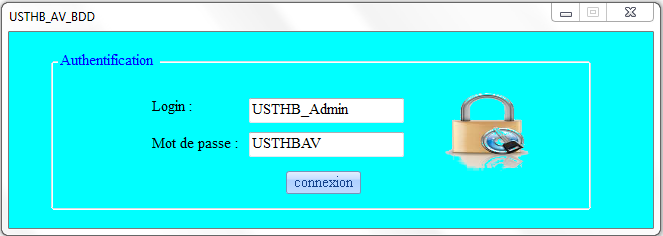
\includegraphics[scale=0.6]{Figures/auth.png}
\caption{L'authentification}
\label{fig :auth} 
\end{center}
\end{figure}

La gestion de la base de signatures permet d'afficher, modifier et supprimer une signature, ainsi que de créer le fichier "info.txt", la figure~\ref{fig :acc} représente la page d'accueil avec  trois fonctionnalités à savoir, la gestion de la base de fichiers légitimes et la gestion de signatures virales et la génération du fichier "info.txt".
\begin{figure}[H]
\begin{center}
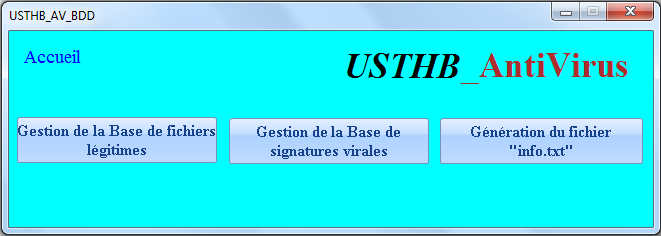
\includegraphics[scale=0.6]{Figures/acc.png}
\caption{La page d'accueil de l'outil de gestion de la base de signatures.}
\label{fig :acc} 
\end{center}
\end{figure}

\subsection{Gestion de la base de fichiers légitimes}
La gestion de la base de fichiers légitimes est composée de deux fonctionnalités :

\subsubsection{Base de fichiers légitimes}
Cette fonctionnalité permet d'afficher la base de fichiers légitimes ainsi que sa taille, la figure~\ref{fig :im3} suivante correspond à une base de 4140 fichiers légitimes.
\begin{figure}[H]
\begin{center}
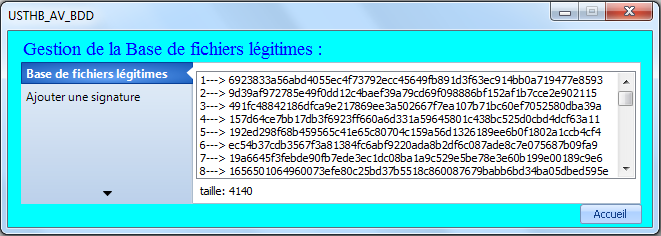
\includegraphics[scale=0.7]{Figures/im3.png}
\caption{La page de la base de fichiers légitimes.}
\label{fig :im3} 
\end{center}
\end{figure}

\subsubsection{Ajouter une signature}
Pour la mise à jour de la base de signatures, l'administrateur peut ajouter une nouvelle signature en suivant les étapes suivantes :\\
\begin{itemize}
\item Sélectionner le fichier légitime à signer en appuyant sur le bouton " … ", qui sera suivi par l'affichage du chemin de fichier sélectionné dans le champ de saisie.
\item Un clic  sur le bouton "ajouter" permet d'insérer le fichier sélectionné dans la base de fichiers légitimes (Figure~\ref{fig :im5})
\end{itemize}
\begin{figure}[H]
\begin{center}
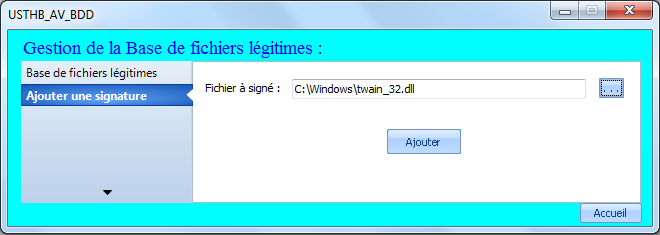
\includegraphics[scale=0.7]{Figures/im5.png}
\caption{La page d'ajouter un fichier légitime.}
\label{fig :im5} 
\end{center}
\end{figure}


\subsection{Gestion de la base de signatures virales}
La gestion de la base de signatures virales est composée de quatre fonctionnalités : 

\subsubsection{Base de malwares} 
Cette fonctionnalité permet d'afficher la base de malwares ainsi que sa taille, la figure~\ref{fig :im12} correspond à une base de 7404 malwares.
\begin{figure}[H]
\begin{center}
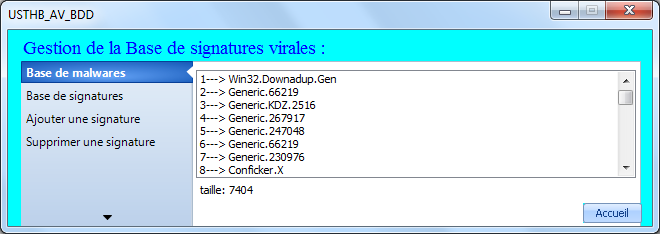
\includegraphics[scale=0.7]{Figures/im12.png}
\caption{La base de malwares.}
\label{fig :im12} 
\end{center}
\end{figure}

\subsubsection{Base de signatures virales}
Cette fonctionnalité permet d'afficher la base de signatures virales, ainsi que sa taille, la figure~\ref{fig :im14} représente une base de 7325 signatures virales :
\begin{figure}[H]
\begin{center}
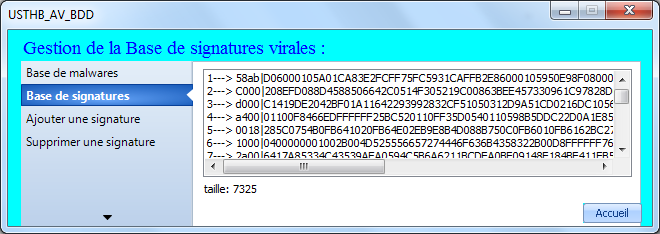
\includegraphics[scale=0.7]{Figures/im14.png}
\caption{La base de signatures virales.}
\label{fig :im14} 
\end{center}
\end{figure}
\subsubsection{Ajouter une signature}
Comme nous avons cité dans le chapitre précédent, une signature virale est composée de quatre champs : un offset, une suite hexadécimale, nom et type de malware, pour ajouter une signature, nous devons suivre les étapes suivantes :
\begin{itemize}
\item Sélectionner le malware à signer avec le bouton "..."
\item Définir l'offset de la suite hexadécimale
\item Récupérer la suite hexadécimale avec le bouton "Récupérer la suite hexadécimale"
\item Définir un nom qui n'existe pas déjà dans la base de signature virale pour ce malware.
\item Définir le type de ce malware 
\item Cliquer sur le bouton "ajouter" pour ajouter la nouvelle signature (Figure~\ref{fig :im7}).      
\end{itemize}
\begin{figure}[H]
\begin{center}
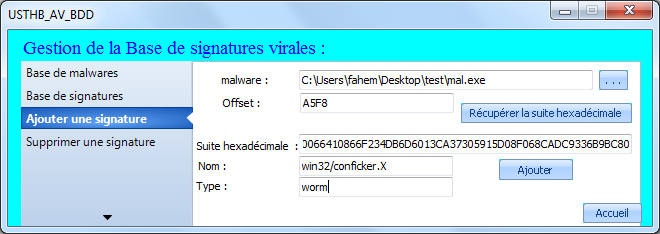
\includegraphics[scale=0.7]{Figures/im7.png}
\caption{Ajouter une signature virale.}
\label{fig :im7} 
\end{center}
\end{figure}

\subsubsection{Supprimer  une signature}
La suppression d'une signature virale nécessite d'indiquer le nom du malware,
dont la signature à supprimer, cette opération s'effectue en deux phases :
\begin{itemize}

\item Saisir le nom du malware 
\item Valider la suppression en cliquant sur bouton "supprimer"(Figure~\ref{fig :im8}).

\end{itemize}
\begin{figure}[H]
\begin{center}
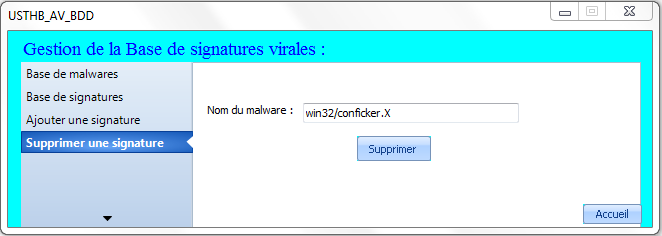
\includegraphics[scale=0.7]{Figures/im8.png}
\caption{Supprimer une signature virale.}
\label{fig :im8} 
\end{center}
\end{figure}
\subsection{Génération du fichier "info.txt"}
Pour créer le fichier "info.txt" l'administrateur doit cliquer sur le bouton "Génération du fichier "info.txt" de la page d'accueil, une fenêtre, contenant des renseignements devant être mis à jour concernant la version de la base de signatures et la version de moteur,s'affiche puis valider par un clic sur le bouton "Générer le fichier" (Figure~\ref{fig :im10}).
\begin{figure}[H]
\begin{center}
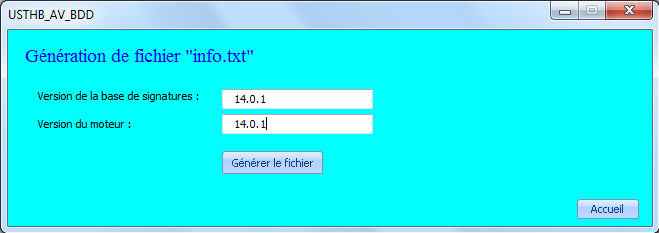
\includegraphics[scale=0.7]{Figures/im10.png}
\caption{Génération du fichier "info.txt".}
\label{fig :im10} 
\end{center}
\end{figure}
\section{Antivirus}

Dans cette partie, nous allons présenter le fonctionnement de notre antivirus.
\subsection{Page d'accueil} 
Dès que l'utilisateur exécute l'antivirus, une page d'accueil sera affichée (Figure~\ref{fig :ant1}), portant les informations et les fonctionnalités suivantes :\\
\begin{itemize}
\item \textbf{Les informations :}
\begin{list}{•}{}
\item Le nom de l'antivirus ( USTHB\_ AntiVirus)
\item L'état actuel de l'antivirus relatif à la dernière mise à jour,dernière analyse, et la version courante de l'antivirus.
\end{list} 
\item \textbf{Les fonctionnalités :}
\begin{list}{•}{}
\item La langue : L'utilisateur coche la langue à utiliser
\item Deux boutons, l'un pour réduire la fenêtre et l'autre pour la fermer
\item Une barre de tâches composée de cinq raccourcis :
\begin{itemize}

\item \textbf{Gestionnaire des tâches : }sert à afficher les programmes, les processus et les services en cours d'exécution sur l'ordinateur et surveiller les performances de l'ordinateur ou pour fermer un programme
\item \textbf{Aide : }permet l'accès au guide d'utilisation
\item \textbf{Exit : }permet de quitter le programme
\item \textbf{Accès internet : }permet un accès rapide sur l'Internet
\item \textbf{Commande cmd : }une fonctionnalité qui offre un point d'entrée pour la saisie de commande Windows.
\end{itemize}
\item Sur la gauche de la page d'accueil, se trouve une barre verticale dont le clic fait apparaitre le menu de l'antivirus.\\
\end{list}
\end{itemize}
La figure~\ref{fig :ant1} montre la page d'accueil de l'antivirus :
\begin{figure}[H]
\begin{center}
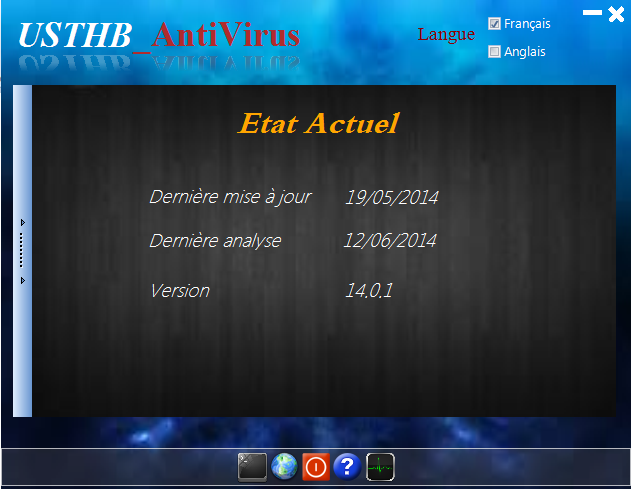
\includegraphics[width=13cm, height=8cm]{Figures/ant1.png}
\caption{Page d'accueil de l'antivirus .}
\label{fig :ant1} 
\end{center}
\end{figure}
\subsection{Page Menu}
Nous trouvons dans cette page les tâches principales de l'antivirus, listées comme suit : Antivirus, Parseur PE, Maintenance, USTHB\_AV, Fichier suspect et protection.\\
La figure~\ref{fig :ant6} montre la page Menu de l'antivirus :
\begin{figure}[H]
\begin{center}
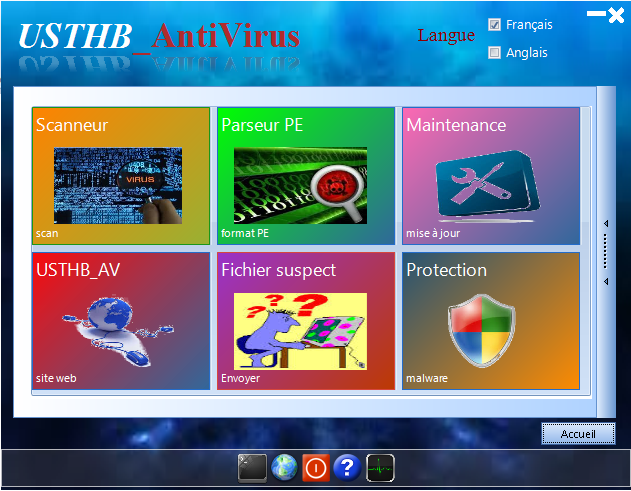
\includegraphics[width=13cm, height=8cm]{Figures/ant6.png}
\caption{Page Menu de l'antivirus .}
\label{fig :ant6} 
\end{center}
\end{figure}
\subsubsection{Scanneur}
L'utilisateur clic sur le champ "Scanneur" pour lancer un scan, une nouvelle page sera affichée(figure~\ref{fig :ant3}), qui contient les quatre types de scan, à savoir ; scan un dossier sélectionné, scan un seul fichier, scan rapide, et scan tout le système.\\
\begin{figure}[H]
\begin{center}
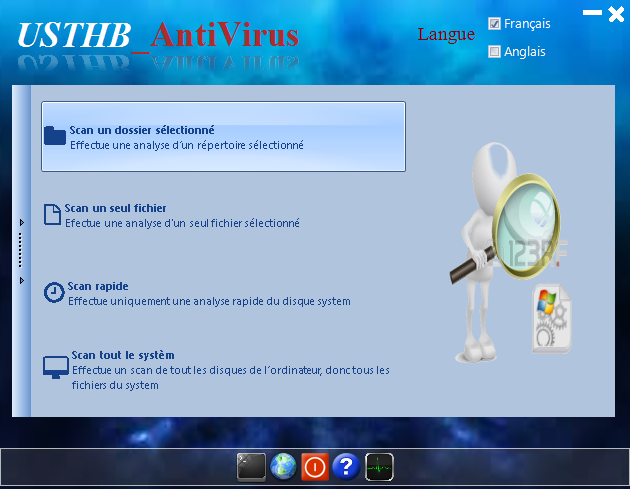
\includegraphics[width=13cm, height=8cm]{Figures/ant3.png}
\caption{Les scans .}
\label{fig :ant3} 
\end{center}
\end{figure}
Selon l'action souhaitable l'utilisateur choisie une des fonctionnalités suivantes :\\

\textit{\textbf{Scan un seul fichier :}}
\begin{list}{•}{}
\item \textbf{Fonctionnement :}\\
Ce champ est choisi une fois le scan aura été pour un seul fichier, le clic sur "scan un seul fichier"  permet d'accéder au chemin de ce fichier, après validation (par un clic sur le bouton OK) le chemin est déclaré dans le champ "fichier analysé".\\
Une fois l'analyse est achevée, trois situations possibles se présentent :\\
\begin{itemize}
\item Le fichier testé est un fichier légitime : un message "le fichier est légitime" est affiché
\item Le fichier testé n'est pas un malware un message "le fichier n'est pan un malware" est affiché
\item Le fichier testé est un malware, dans ce cas, des informations suivantes sont affichées :
\begin{list}{*}{}
\item Le type de malware détecté
\item Une image relative à ce type de malware
\item Une sonnerie d'alerte 
\item Un lien vers la page des résultats d'analyse.\\
\end{list} 
\end{itemize}

La figure~\ref{fig :im14} représente un test d'un fichier "adobe.exe" : \\
\begin{figure}[H]
\begin{center}
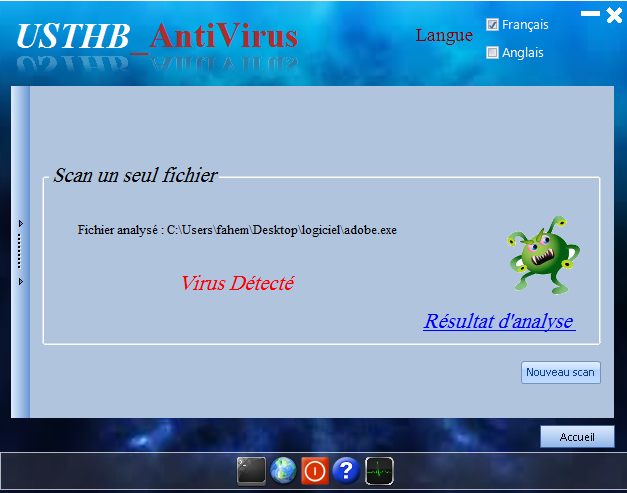
\includegraphics[width=13cm, height=8cm]{Figures/ant14.png}
\caption{Un virus détecté .}
\label{fig :ant6} 
\end{center}
\end{figure}
  
L'utilisateur peut abandonner ou lancer un  nouveau scan par un clic sur le bouton "Nouveau scan", ou visualiser les résultats d'analyse par un clic sur le lien "Résultats d'analyse".
\item \textbf{Résultat d'analyse :}
Après un clic sur le lien "Résultats d'analyse", ces résultats s'affichent dans une nouvelle page, ainsi que les actions qui peuvent être appliquées à ce malware, à savoir ; supprimer, mettre en quarantaine, et ne rien faire, la figure~\ref{fig :ant11} correspond aux résultats d'analyse du fichier "adobe.exe".\\
\begin{figure}[H]
\begin{center}
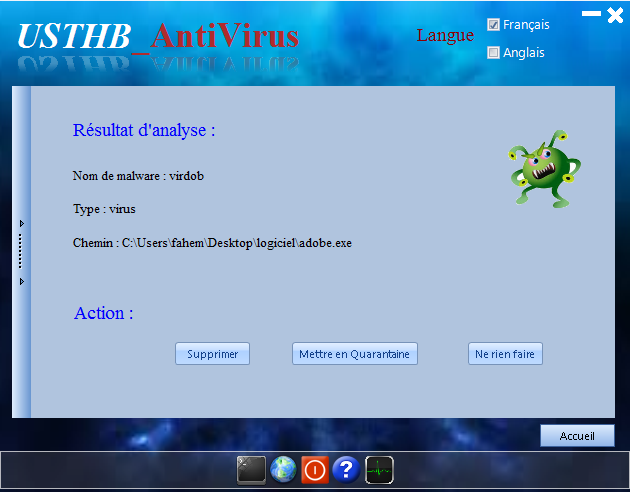
\includegraphics[width=13cm, height=8cm]{Figures/ant11.png}
\caption{L'affichage des résultats d'analyse .}
\label{fig :ant11} 
\end{center}
\end{figure}
\end{list}

\textit{\textbf{Scan un dossier sélectionné : }}
\begin{list}{•}{}
\item \textbf{Fonctionnement : }\\
Ce champ est choisi une fois le dossier à scanner est bien précis, le clic sur "scan un dossier sélectionné"  fait apparaitre une nouvelle page (figure)\\
\begin{itemize}
\item Le dossier à scanner est sélectionné en cliquant sur le bouton " … " cette action permet un accès au chemin de ce dossier 
\item après validation (par un clic sur le bouton OK) le chemin est déclaré dans le champ "répertoire analysé"
\item Au cours de l'analyse des informations ponctuelles vont s'afficher à savoir:
\begin{list}{*}{}
\item Une barre de progression : déclare le taux d'avancement de l'opération
\item Fichier examiné : dans ce champ s'affiche le chemin du fichier en cours d'analyse
\item Temps d'analyse : dans ce champ s'affiche le temps écoulé depuis le début d'analyse
\item Nombre totale : dans ce champ s'affiche le nombre total des fichiers à analyser
\item Malware détecté : dans ce champ s'affiche le nombre final des malwares détectés.
\end{list}

\item A  tout moment l'utilisateur peut effectuer un nouveau type de scan par un simple clic sur le bouton "nouveau scan" qui permet le retour à la page scanneur ou retourner carrément à la page d'accueil  par le bouton "accueil" 
\item Une fois l'analyse est achevée, deux situations possibles se présentent :
\begin{list}{*}{}

\item Aucun malware n'est détecté : un message signalant l'absence des malwares s'affiche 
\item Présence des malwares : une sonnerie d’alerte est déclenchée, signalant la présence de ces malwares, le nombre de ces derniers sera communiqué dans le champ " malware détecté", un nouveau bouton "Résultat d'analyse" sera affiché, pour accéder à ces résultats, il suffit de cliquer sur ce bouton.\\
\end{list}
\end{itemize}
La figure correspond à une analyse d'un dossier nommé logiciel, dont le chemin est \url{C:\User\fahem\Desktop\logiciel}, le résultat de l'analyse est :\\

\begin{itemize}
\item Dernier fichier examiné nommé adobe.exe
\item Temps d'analyse : 0 :01 :47
\item Nombre total : 12
\item Malware détecté : 3

\end{itemize}
\begin{figure}[H]
\begin{center}
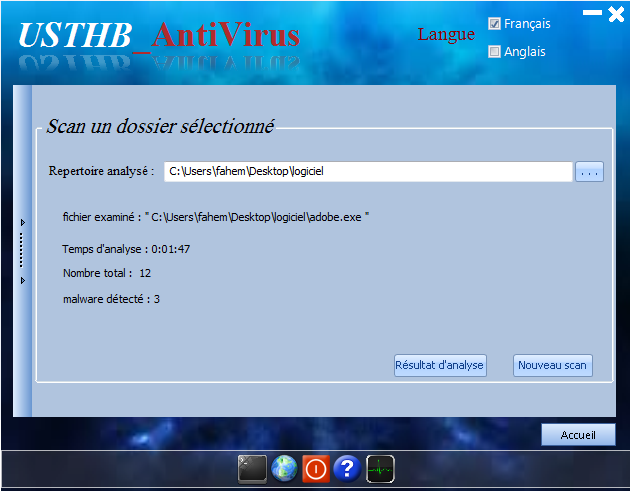
\includegraphics[width=13cm, height=8cm]{Figures/ant13.png}
\caption{Scan un dossier sélectionné .}
\label{fig :ant13} 
\end{center}
\end{figure}
\item \textbf{Résultat d'analyse : }\\
Après un clic sur le bouton "résultat d'analyse", les résultats s'affichent dans une grille, avec deux choix de traitement :\\
\begin{itemize}
\item La suppression ou la mise en quarantaine des malwares un par un, et ce, comme suit :
sélectionner le malware à supprimer ou à  mettre en quarantaine, après on valide l'action par le bouton "Supprimer" ou "mettre en quarantaine", si l'action choisie est faisable, le malware ne s'affiche plus dans la grille, et vis versa  

\item Une action collective  de traitement  pour tous les malwares détectés, à savoir ; supprimer,  mettre en quarantaine, ou ne rien faire, qui sera choisie dans le  CombBox, suivie d'une validation par le bouton "Appliquer".\\
\end{itemize}


Le bouton "Quitter" permet d'abandonner les résultats d'analyse, et un retour automatique  à la page antivirus(Figure~\ref{fig :ant12}).\\
\end{list}
\begin{figure}[H]
\begin{center}
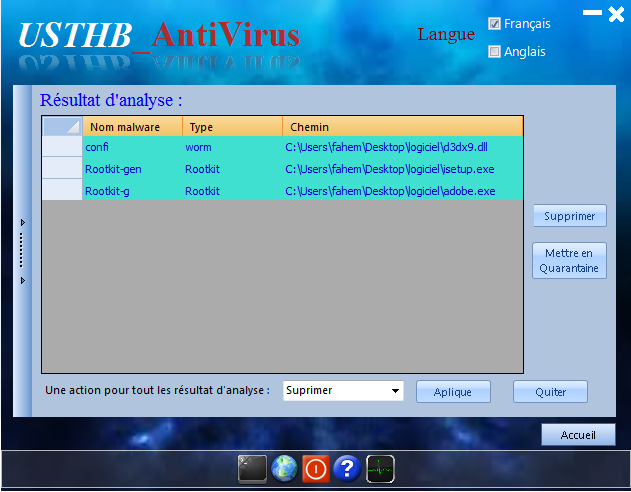
\includegraphics[width=13cm, height=8cm]{Figures/ant12.png}
\caption{Résultats d'analyse d'un dossier sélectionné .}
\label{fig :ant12} 
\end{center}
\end{figure}
\textit{\textbf{Scan rapide : }}\\

Le fonctionnement de ce scan est le même que le scan d'un dossier sélectionné, sauf que la cible d'analyse dans le scan rapide est prédéfinie "C:\", contrairement au scan d'un dossier sélectionné ou l'utilisateur doit sélectionner la cible d'analyse.\\

        
Le traitement des résultats d'analyse dans le scan rapide est basé sur les mêmes principes de scan d'un dossier sélectionné.\\
\textit{\textbf{Scan tout le système }}\\

Le fonctionnement et le traitement des  résultats de ce scan sont les mêmes que le scan rapide, sauf que dans le scan de tout le système, l'ensemble des disques de l'ordinateur seront analysés.

\subsubsection{Parseur PE}

Pour observer le contenu d'un fichier exécutable, l'utilisateur clique sur le champ "Parseur PE" de la page Menu, une nouvelle page apparait, ensuite l'utilisateur doit cliquer sur le bouton " … "   afin d'accéder au chemin du fichier à analyser, après validation (par un clic sur le bouton OK) le chemin est déclaré dans le champ "fichier à analyser", deux cas possibles ont été constatés :\\

\begin{list}{•}{}
\item Le fichier analysé à un format PE non valide : un message "Format PE non valide"
\item Le fichier analysé à un format PE valide : les résultats ; EntryPoint, PE détail, les sections PE,  la liste des fonctions API importées et les éventuels packers utilisés 
seront affichés dans un nouveau champ.\\
\end{list}
La figure~\ref{fig :ant7} représente les résultats d'analyse d'un fichier PE valide :
\begin{figure}[H]
\begin{center}
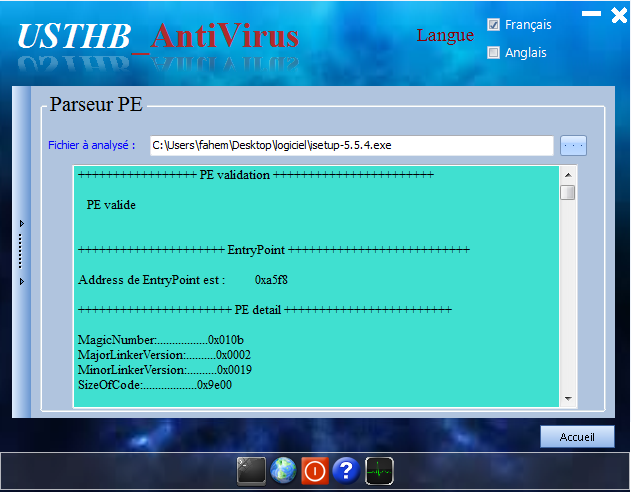
\includegraphics[width=13cm, height=8cm]{Figures/ant7.png}
\caption{Le parseur PE de l'antivirus .}
\label{fig :ant7} 
\end{center}
\end{figure}

\subsubsection{Maintenance}
Pour effectuer une mise à jour, l'utilisateur doit cliquer sur le champ "Maintenance" de la page menu, cette action va faire apparaitre une nouvelle page (Figure) comportant :\\

\begin{list}{•}{}
\item Deux boutons, le premier intitulé "mise à jour de la base de signatures"  le deuxième "mise à jour du programme"
\item Des renseignements concernant la version actuelle de la base de signatures et de programme ainsi que le nombre de signatures
\item Un message encourageant la mise à jour.\\
\end{list}
La mise à jour se déroule par un clic sur l'un des boutons cités précédemment, deux cas sont possibles :\\
\begin{list}{•}{}
\item Il n'existe pas une nouvelle mise à jour : dans ce cas un message "votre antivirus est déjà mis à jour" est affiché
\item Il existe une mise à jour : une barre de progression, qui déclare le taux d'avancement de l'opération, une fois cette dernière est terminée, un message "mise à jour effectuée avec succès" est affiché, en cas d'échec, ce dernier sera déclaré via un message. \\
\end{list}
La figure~\ref{fig :ant5} présente la page de mise à jour de l'antivirus :
\begin{figure}[H]
\begin{center}
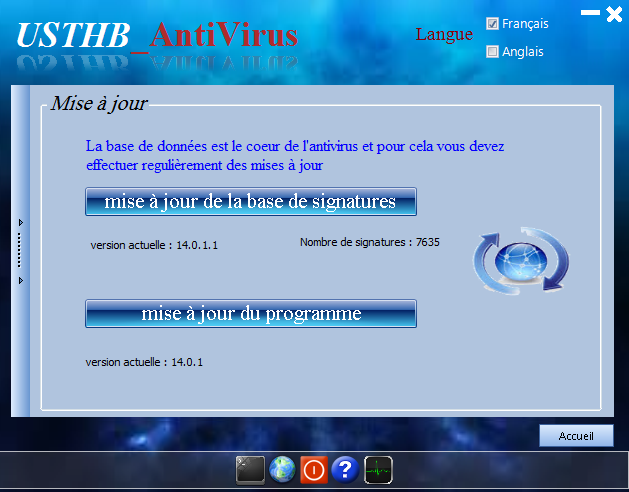
\includegraphics[width=13cm, height=8cm]{Figures/ant5.png}
\caption{La mise à jour de l'antivirus .}
\label{fig :ant5} 
\end{center}
\end{figure}
\subsubsection{USTHB\_AV} 
Pour avoir les dernières actualités sur l'antivirus, télécharger le fichier d'installation de l'antivirus, guide d'utilisation,...\\
L'utilisateur doit cliquer sur le champ "USTHB\_AV" de la page Menu,  cette action permet à l'utilisateur d'accéder au site web de l'antivirus \url{http://usthbav.jimdo.com/}(Figure~\ref{fig :ant2}):
\begin{figure}[H]
\begin{center}

\includegraphics[width=16cm, height=6cm]{Figures/web.png}
\caption{Le site web de l'antivirus .}
\label{fig :ant2} 
\end{center}
\end{figure}
\subsubsection{Fichier suspect}
Pour envoyer un fichier suspect, l'utilisateur doit cliquer sur le champ "Fichier suspect" de la page Menu, cette action va faire apparaitre une nouvelle page (Figure) portant un message décrit les étapes obligatoires à suivre pour envoyer un fichier suspect, qui sont :\\
\begin{list}{•}{}

\item Archiver le fichier suspect à envoyer en ".rar"
\item Définir un mot de passe pour le fichier archivé
\item Cliquer sur le bouton " … "   afin d'accéder au chemin du fichier suspect à envoyer, après validation (par un clic sur le bouton OK) le chemin est déclaré dans le champ "fichier à envoyer"
\item Décrire le fichier suspect au niveau de champ "Sujet" 
\item Accompagner le fichier archivé par le mot de passe de décompression, au niveau de champ "mot de passe de décompression"   
\item Valider l'envoi du fichier suspect par un clic sur le bouton "Envoyer".\\
\end{list}
Après la validation de l'envoi du fichier suspect, une barre de progression sera affichée,  une fois cette dernière est terminée, un message "Fichier envoyé avec succès" est affiché, en cas d'échec, ce dernier sera déclaré via un message.\\

La figure~\ref{fig :ant4} décrit l'envoi d'un fichier suspect, nommé "suspect.rar",  sujet "fichier suspect" et un mot de passe de décompression "Ss000000".
\begin{figure}[H]
\begin{center}
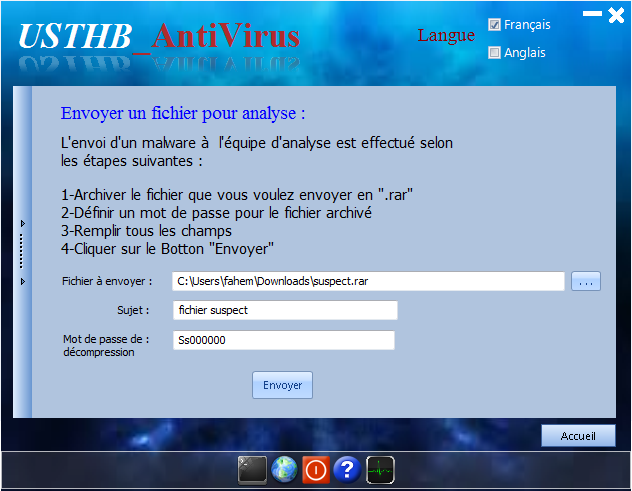
\includegraphics[width=13cm, height=8cm]{Figures/ant4.png}
\caption{L'envoie d'un fichier suspect .}
\label{fig :ant4} 
\end{center}
\end{figure}

\subsubsection{Protection} 
Pour visualiser les informations relatives à l'antivirus, l'utilisateur doit cliquer sur le champ "Protection" de la page Menu, cette action va faire apparaitre une nouvelle page,  portant trois paramètres, détection, informations et quarantaine, indiqué ci- dessous :\\

\begin{list}{•}{}
\item \textbf{Détection : } permet à l'utilisateur de voir la liste des malwares classée par leur nom et type, détectés par l'antivirus(Figure~\ref{fig :ant8})
\begin{figure}[H]
\begin{center}
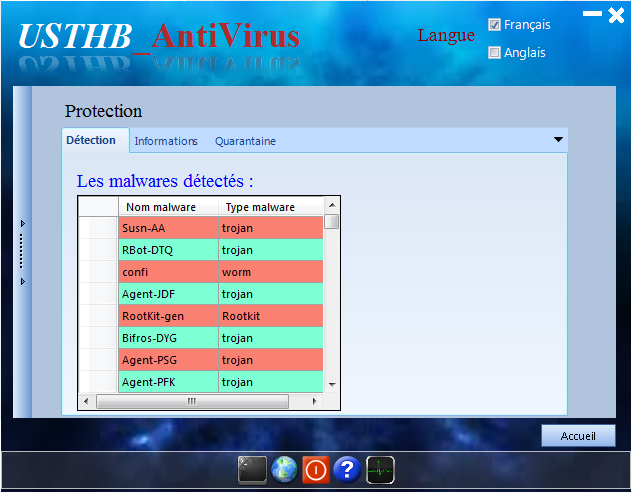
\includegraphics[width=13cm, height=8cm]{Figures/ant8.png}
\caption{Les malwares détectés par l'antivirus .}
\label{fig :ant8} 
\end{center}
\end{figure}
\item \textbf{Information : }Cette partie sert à indiquer les informations relatives à la version actuelle de l'antivirus, qui sont : version de la base virale, nombre de signatures, nombre de malwares détectés et la version du moteur (Figure~\ref{fig :ant9})
\begin{figure}[H]
\begin{center}
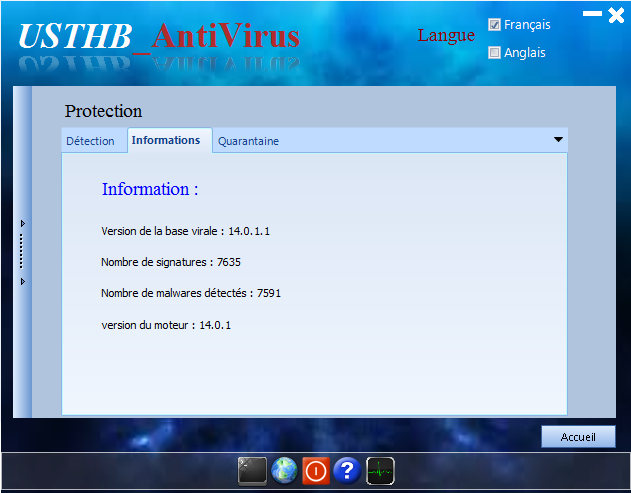
\includegraphics[width=13cm, height=8cm]{Figures/ant9.png}
\caption{Les informations relatives à l'antivirus .}
\label{fig :ant9} 
\end{center}
\end{figure}
\item \textbf{Quarantaine : }Cette option permet à l'utilisateur de visualiser la liste des malwares, déjà mis en quarantaine, la figure~\ref{fig :ant10} représente une quarantaine de trois malwares.  
\begin{figure}[H]
\begin{center}
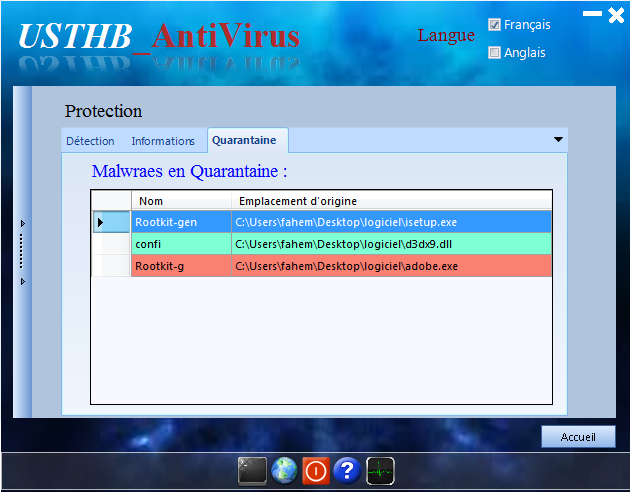
\includegraphics[width=13cm, height=8cm]{Figures/ant10.png}
\caption{Quarantaine .}
\label{fig :ant10} 
\end{center}
\end{figure}
\end{list}
\section{L'accès à l'interface de l'antivirus}
L'utilisateur peut accéder a l'antivirus via trois méthodes différentes :\\
\begin{list}{•}{}

\item \textbf{A partir du Menu démarrer : }la figure~\ref{fig :demar} présente l'apparence de l'antivirus dans le Menu démarrer.
\begin{figure}[H]
\begin{center}
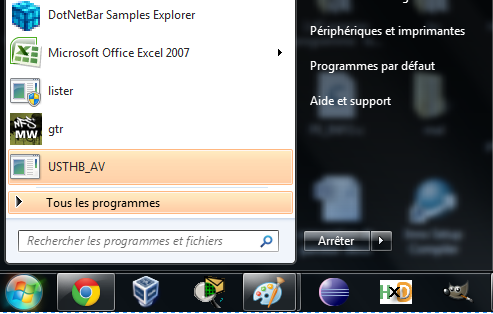
\includegraphics[width=11cm, height=6cm]{Figures/demar.png}
\caption{Menu démarrer.}
\label{fig :demar} 
\end{center}
\end{figure}

\item \textbf{A partir d'un raccourci : }voir la figure~\ref{fig :racc}
\begin{figure}[H]
\begin{center}
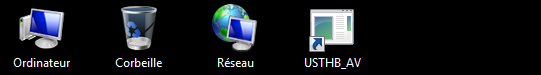
\includegraphics[width=11cm, height=1.5cm]{Figures/racc.png}
\caption{Raccourci au Bureau.}
\label{fig :racc} 
\end{center}
\end{figure}
\item \textbf{A partir de la zone de notification : } la figure~\ref{fig :systray} représente l'apparence de notre antivirus au niveau de la zone de notification ainsi que les tâches que l'on peut effectuer depuis cette zone.
\begin{figure}[H]
\begin{center}
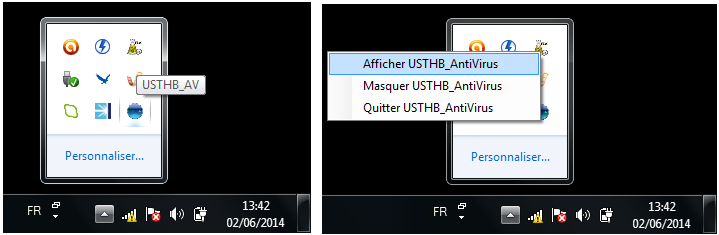
\includegraphics[width=13cm, height=4cm]{Figures/systray.png}
\caption{Zone de notification "Systray".}
\label{fig :systray} 
\end{center}
\end{figure}
\end{list}
\subsection*{Lancement de l'antivirus au démarrage de Windows}
La figure~\ref{fig :run} représente la liste des programmes à lancer au démarrage de Windows
\begin{figure}[H]
\begin{center}
\includegraphics[width=10cm, height=5cm]{Figures/run.png}
\caption{Lancement de l'antivirus au démarrage de windows.}
\label{fig :run} 
\end{center}
\end{figure}
\section{Conclusion}
Dans ce chapitre nous avons vu l'ensemble de fonctionnalités de l'antivirus, côté administrateur "gestion de la base de signatures", côté utilisateur "antivirus". \\

Puis, à travers les impressions écrans, nous avons vu les interfaces, de l'application, illustrant chacune une fonctionnalité. 

\chapter{Analyse de malwares}
\section{Introduction}
L'analyse de malwares (malware analysis) est aujourd’hui devenue une activité très importante dans le cadre de la gestion des incidents de sécurité informatique. Les organisations qui prennent sérieusement en compte la sécurité de leurs réseaux sont souvent confrontées a des fichiers suspects capturés grâce à leurs antivirus, IDS et systèmes de supervision sécurité, ou encore lors d'analyses forensics. Il est alors nécessaire d'analyser rapidement ces fichiers pour déterminer s'il s'agit de code malveillant connu, d'une attaque ciblée ou bien d'un faux positif. Connaître le comportement d'un malware est capital pour déterminer si d'autres machines sur le réseau peuvent être compromises ou non, et pour décider comment réagir.\\


L'analyse statique de code exécutable par désassemblage a beaucoup de succès et permet d'obtenir d'excellents résultats, cependant la complexité de ce processus demande un long apprentissage, beaucoup de temps et d'énergie. De plus il n'est pas rare de rencontrer des codes malveillants protégés contre le désassemblage et le débogage, ce qui peut ralentir considérablement l'analyse.\\


L'analyse dynamique de code malveillant est une autre méthode qui consiste à faire exécuter un échantillon de code sur une plate-forme conçue pour observer toutes ses actions. Dans la plupart des cas, c'est une approche très efficace et rapide pour déterminer la nature et le comportement du code malveillant, au moins dans un premier temps.

\section{Objectifs de l'analyse de malwares}
Voici quelques-uns des objectifs habituels d'une analyse de malware :\\


\begin{itemize}
\item Vérifier si un fichier suspect est effectivement malveillant ou s'il s'agit d'un faux positif
\item Déterminer s'il s'agit d'un code malveillant générique (connu ou non) ou bien d'une attaque ciblée
\item Obtenir des informations sur la source de l'attaque
\item Déterminer toutes les actions du code malveillant sur le système local : fichiers créés/modifiés/supprimés, processus lancés/stoppés, clés de registre, services installés, ...
\item Déterminer toutes ses actions sur le réseau : connexions sortantes, réplication, serveur en écoute, ...
\item Déterminer ses "fonctionnalités" malveillantes : virus, ver, cheval de Troie, porte dérobée, bombe logique, rootkit, keylogger, téléchargement, relais de spam, déni de service, botnet, ...
\item Déterminer quelles sont les machines ciblées et lesquelles pourraient être vulnérables ou déjà compromises sur le réseau
\item Fournir des informations pour mieux cibler une éventuelle analyse forensics d'autres machines (noms de processus, empreintes MD5 de fichiers, clés de registre, mots clés, ...)
\item Décider quelles actions entreprendre pour gérer l'incident
\item Comprendre comment la compromission s'est déroulée afin d'améliorer les protections à l'avenir.\\
\end{itemize}

\section{Où trouver des malwares ?}

Il existe toute une communauté autour de l'analyse de malwares : forums, sites, blogs, etc. Certains de ces sites mettent à disposition des échantillons permettant d'effectuer des analyses. Quelques adresses :
\begin{list}{•}{}
\item \textbf{KernelMode : }Forum d’échange et d’analyse de malwares. Met à disposition des lecteurs des échantillons~\cite{mal1} 
\item  \textbf{Malware.lu : }Excellent site mettant à disposition des échantillons de malwares et proposant des analyses~\cite{mal2}
\item \textbf{Contagio Exchange : }Site permettant d'échanger et de télécharger des malwares~\cite{mal3}
\item \textbf{CrowdRE : }Plate-forme collaborative d'analyse de malwares~\cite{mal4}
\item \textbf{VadeRetro Sales malwares : }Articles et tutoriaux sur les malwares~\cite{mal5}
\item \textbf{Malekal's Site : }Excellent site consacré à l'entraide informatique. De nombreux exemples d'analyses comportementales~\cite{mal6}
\item \textbf{Malware Analysis \& Diagnostics : }Analyse de malwares~\cite{mal7} 
\item \textbf{FireEye Malware Intelligence Lab : }Site de recherche et d'analyses de malwares~\cite{mal8}
\item \textbf{Evil3ad : }Site d'analyse de malwares~\cite{mal9}
\item \textbf{M86SecurityLabs : }Site consacré aux attaques (malwares, cybercriminalité)~\cite{mal10}
\item \textbf{Fun in malwares analysis :} Tutoriaux sur l'analyse de malwares~\cite{mal11}.\\
\end{list}



Les blogs des compagnies antivirales publient aussi de nombreuses analyses :
\begin{list}{•}{}
\item \textbf{Blog de Kaspersky : }~\cite{blog1}
\item \textbf{Blog d'Eset : }~\cite{blog2} 
\item \textbf{Blog de Norton : }~\cite{blog3}
\item \textbf{Blog de Sophos : }~\cite{blog4}.\\
\end{list}
\section{Construire un laboratoire sécurisé d'analyse de malwares}

Dans la section précédente, nous avons vu différentes méthodes pour récupérer des malwares. Maintenant comment les étudier en toute sécurité ? Il est bien sûr "impensable" de les exécuter et de les analyser sur un poste de travail. Il convient donc de créer un environnement spécial permettant de les analyser en toute sécurité.
\subsection{La virtualisation}
La virtualisation a révolutionné de nombreux domaines de l’informatique dont le domaine de l’analyse des malwares. Il devient ainsi simple et rapide de tester des malwares dans des environnements contrôlés afin de découvrir leurs actions.\\

Parmi les outils les plus utilisés dans le domaine de la virtualisation personnelle, nous pouvons citer principalement \textbf{Vmware}~\cite{vm}(payant) ainsi que \textbf{VirtualBox}~\cite{vbox} (gratuit). Par contre certains malwares possèdent des fonctionnalités de détection d'environnements virtuels et stoppent leur exécution.
\subsubsection{Avantages de la virtualisation}
\begin{itemize}
\item \textbf{Coût et flexibilité :} une seule machine physique permet de simuler deux machines ou plus, et de construire différentes
architectures réseau suivant les besoins.
\item \textbf{Sécurité :} les machines virtuelles peuvent être connectées par un réseau virtuel totalement indépendant de tout réseau
opérationnel, sans risque d'infecter d'autres machines.
\item \textbf{Rapidité et efficacité :} une machine virtuelle peut être stoppée, restaurée et redémarrée en quelques secondes.
\item \textbf{Facilité d'emploi :} n'importe quel état de fonctionnement peut être sauvegardé dans un "snapshot" en quelques secondes. Il est ensuite très simple de restaurer tout snapshot précédent, et de comparer plusieurs états entre eux.
\item Les machines virtuelles peuvent être facilement copiées, dupliquées et modifiées pour constituer une bibliothèque de toutes les versions d’un système d’exploitation ou d’une application.
\end{itemize}
\subsubsection{Inconvénients de la virtualisation}
\begin{itemize}
\item Il existe de nombreuses techniques connues utilisables par des malwares pour détecter s'il s'exécutent dans une machine virtuelle. Dans ce cas ils peuvent éviter de s'exécuter ou perturber l'analyse.
\item Certains environnements de virtualisation peuvent être vulnérables et permettre à un code malveillant spécifiquement conçu de "s'échapper" d'une machine virtuelle pour compromettre le système hôte. Il est donc utile de prendre quelques précautions
lors de toute exécution de code malveillant.
\end{itemize}


\subsection{Considérations du système d'exploitation}
Les malwares comportent radicalement différent selon le système d'exploitation lequel sont exécutés sur. Certains malwares ne peuvent fonctionner que sur les systèmes d'exploitation Microsoft Windows Server, tandis que d'autres programmes malveillants ne peuvent fonctionner que sur des versions spécifiques du noyau Linux. Malware qui est installé sur un hôte Microsoft Windows Vista peut crasher complètement le système, tandis que le même malware installé sur un système Microsoft Windows 7 pourrait rejoindre un réseau de zombies (botnet). C'est une nécessité d'avoir une variété de systèmes d'exploitation disponibles lors de l'analyse des programmes malveillants. Donc il faut avoir différents systèmes d'exploitation comme Microsoft Windows XP, Microsoft Windows 7, Microsoft Windows Server 2003, et l'une des distributions Linux les plus populaires modernes comme Ubuntu pour servir d'hôtes infectés.
\subsection{L'isolement du réseau}
Des précautions supplémentaires doivent être prises en ce qui concerne l'emplacement des hôtes d'analyse des malwares sur le réseau. Les vers (Worms) et autres types de programmes malveillants peuvent avoire la fonction "auto-réplication", il est donc très probable que l'exécution de malware sur une machine du réseau peut conduire à d'autres hôtes sur ce réseau.\\
Un argument supplémentaire pour isoler les machines de laboratoire de l'Internet est d'empêcher les auteurs des logiciels malveillants de savoir l'existence de l'analyste. Il est tout à fait probable que le malware exécuté est configuré pour "phone home" à une commande \& contrôle le serveur qui permet à l'auteur de savoir  que vous avez exécuté le malware. À ce stade, l'attaquant pourrait commencer l'exécution de commandes sur le système de laboratoire pour tenter de désactiver ou déjouer les tentatives d'analyse.\\

La figure~\ref{fig :lab} donne un exemple de laboratoire d'analyse de malwares.
\begin{figure}[H]
\begin{center}
\includegraphics[scale=0.65]{Figures/lab.png}
\caption{Exemple d'un laboratoire d'analyse de malwares.}
\label{fig :lab} 
\end{center}
\end{figure}

\subsection{Les distributions dédiées à l'analyse de malwares}


Il existe des distributions consacrées spécialement à l'analyse de malwares, une d'elle est particulièrement connue : \textbf{REMnux}(Figure~\ref{fig :rem}). C'est une distribution Ubuntu conçue spécialement pour l'analyse de malwares. Elle contient des outils pour analyser la mémoire, des documents pdf vérolés, le réseau, ...\\
\begin{figure}[H]
\begin{center}
\includegraphics[scale=0.5]{Figures/remnux.png}
\caption{Remnux, distribution pour l'analyse de malwares.}
\label{fig :rem} 
\end{center}
\end{figure}


Il existe aussi une distribution nommée \textbf{Zero Wine}(Figure~\ref{fig :wine}) qui permet d'analyser le comportement d'un malware : le malware est exécuté dans un bac à sable (sandbox) puis de nombreux rapports sont générés.
\begin{figure}[H]
\begin{center}
\includegraphics[scale=0.7]{Figures/wine.jpg}
\caption{Distribution ZeroWine pour l'analyse de malwares.}
\label{fig :wine} 
\end{center}
\end{figure}
\section{Les méthodologies d'analyse de malwares}
\subsection{L'analyse statique}
\subsubsection{Définition}
L'analyse statique de malwares consiste à explorer le contenu des fichiers suspects à l'aide de divers outils, dans le but d'extraire le maximum d'informations sans exécuter le code malveillant qu'ils pourraient contenir. A ce stade il s'agit uniquement
d'observer le contenu "visible". Le premier outil à employer dans ce cas est
toujours un afficheur texte/hexadécimal.\\

Une analyse directe de ce type permet souvent de révéler beaucoup d'informations utiles grâce aux chaînes de caractères qui apparaissent en clair, aux entêtes de fichiers, aux méta-données, etc. Il est même parfois possible d'extraire des données camouflées par des méthodes simples (i.e. "XOR"), sans recourir à des méthodes d'analyse sophistiquées. Dans le cas de document malformés (par exemple des exploits pour MS Office, PDF, ...), des outils de "file carving" peuvent souvent extraire les fichiers exécutables malveillants stockés à l'intérieur.\\

Voici le type d'informations utiles qu'il est souvent possible d'extraire :\\
\begin{itemize}


\item Types de fichiers
\item Présence de code malveillant connu ou non
\item Adresses IP, URLs, noms de domaines ou de machines (cibles du code malveillant, serveur de téléchargement ou bien connexion retour vers un serveur de contrôle)
\item Date de création des fichiers, auteur, organisation et autres informations (méta-données dans les documents)
\item Encodages utilisés (qui peuvent trahir une provenance exotique)
\item Présence possible de shellcodes ("NOP sleds" : typiquement une longue suite d'octets 0x90)
\item Mots clés particuliers qui peuvent indiquer une attaque ciblée : nom de l'entreprise, noms de serveurs, d'applications ou d'utilisateurs spécifiques, mots de passe internes, etc.

\end{itemize}
\subsubsection{Le désassemblage}
Le désassemblage (reverse engineering) consiste à ouvrir un fichier exécutable avec des outils tel que \textbf{IDA pro}, ou \textbf{Metasm} par exemple afin de retrouver et d'analyser le code assembleur correspondant au contenu binaire du fichier. Certains outils avancés peuvent même offrir des fonctions de décompilation permettant de reconstruire le code source de haut niveau employé au départ (en général C).\\
En analysant le code, il est ainsi possible d'étudier le comportement de chaque partie du programme et d'en déduire les fonctionnalités.\\

L'avantage de cette méthode est qu'en théorie il est possible d'analyser tout le code, même celui ne s'exécutant que sous certaines conditions particulières. De nombreux malwares ont par exemple des fonctions pour ne pas s'exécuter dans un environnement virtuel, ce qui empêche une analyse dynamique. Dans ce cas, seul le désassemblage peut permettre l'analyse du malware. Il est aussi possible de trouver d'éventuelles routines d'obfuscations employées afin de masquer les données sensibles du code malveillant (mot de passe, clés de chiffrement, adresse des serveurs, etc.)\\

Cependant le désassemblage a quelques inconvénients :\\

\begin{itemize}
\item Il  \textbf{nécessite de grandes compétences} afin de pouvoir lire et d'analyser du code assembleur. Il faut connaître les correspondances systèmes entre le code, les langages de haut niveau et les appels systèmes
\item \textbf{L'analyse complète d'un fichier peut représenter beaucoup de temps} (de plusieurs jours à plusieurs semaines), de compétences et d'énergie selon la taille et la complexité du code
\item \textbf{Certains malwares sont protégés contre le désassemblage} à l'aide de techniques de compression et de chiffrement. Ces protections, jamais parfaites, peuvent néanmoins ralentir l'analyse et demander beaucoup d'efforts pour être cassées.
\end{itemize}
\subsubsection{Les outils et les services d'analyse statique}
\begin{itemize}
\item \textbf{La commande file : }file est une commande d'UNIX qui permet de déterminer le type d'un fichier.\\
Pour chaque fichier valide passé en paramètre, file tente de déterminer le type de données qu'il contient et affiche cette information et éventuellement d'autres informations comme les dimensions pour une image ou les codecs.\\
La figure~\ref{fig :file} donne un exemple d'utilisation de la commande file :
\begin{figure}[H]
\begin{center}
\includegraphics[scale=0.7]{Figures/file.png}
\caption{Utilisation de la commande file.}
\label{fig :file} 
\end{center}
\end{figure}
\item L'outil \textbf{md5sum : }est un utilitaire en ligne de commande qui permet de vérifier l'intégrité d'un fichier. En effet, il permet de récupérer et comparer des empreintes MD5 des fichiers.\\
La figure~\ref{fig :md5} donne un exemple d'utilisation de l'outil md5sum :
\begin{figure}[H]
\begin{center}
\includegraphics[scale=0.7]{Figures/md5sum.png}
\caption{L'outil md5sum.}
\label{fig :md5} 
\end{center}
\end{figure}
\item \textbf{Antivirus scaninig :}Après la récupération de hash md5 de malware qui va nous permettre de savoir si ce malware a été déjà analysé par une autre personne. Pour ce
faire, on peut trouver des sites qui permettent d'accomplir cette tâche. Il suffit d'entrer le fichier et il va vérifier s'il s'agit d'un malware connu ou non. On peut citer comme exemple le site suivant \url{www.virustotal.com} qui permet d'analyser le fichier avec 52 antivirus différents. Cette étape est très importante dans le but de ne pas perdre du temps dans l'analyse d'un malware déjà connu.\\
La figure montre la page web VirusTotal.com :
\begin{figure}[H]
\begin{center}
\includegraphics[scale=0.5]{Figures/vit.png}
\caption{Aperçu sur l'interface du site www.virustotal.com.}
\label{fig :vit} 
\end{center}
\end{figure}
\item \textbf{Strings de Sysinternals suite : }Recherche pour ANSI et UNICODE chaînes dans les fichiers.\\
La figure~\ref{fig :strings} montre un exemple d'utilisation de l'outil strings :
\begin{figure}[H]
\begin{center}
\includegraphics[scale=0.7]{Figures/strings.png}
\caption{L'outil strings de Sysinternals suite.}
\label{fig :strings} 
\end{center}
\end{figure}
\item \textbf{PEiD : }Il détecte les packers et les compilateurs les plus courants pour les fichiers PE. Il est actuellement possible de détecter plus de 470 signatures différentes dans les fichiers portable exécutable.\\
La figure~\ref{fig :pei} montre le programme PEiD.
 \begin{figure}[H]
\begin{center}
\includegraphics[scale=0.8]{Figures/PEID.png}
\caption{L'interface de PEiD.}
\label{fig :pei} 
\end{center}
\end{figure}
\item \textbf{Les désassembleurs : }Parmi les outils les plus connus pour le désassemblage, il y a bien sûr \textbf{IDA}. IDA  est un désassembleur commercial très utilisé en rétro-ingénierie. Il supporte une grande variété de formats exécutables pour différents processeurs et systèmes d'exploitation.\\
IDA permet de passer du code binaire du malware vers son code assembleur. De plus, on peut lui ajouter le plugin Hex-Ray qui va nous permettre de faire la décompilation (c'est-à-dire revenir au code C).\\
La figure~\ref{fig :ida} montre le programme IDA :
\begin{figure}[H]
\begin{center}
\includegraphics[scale=0.42]{Figures/ida.png}
\caption{Interface d'IDA Pro Free.}
\label{fig :ida} 
\end{center}
\end{figure}
\end{itemize}
\subsection{L'analyse dynamique}
\subsubsection{Définition}
Contrairement à l'analyse statiques, l'analyse dynamique consiste à exécuter réellement le code malveillant dans un environnement adéquat afin d'observer toutes ses actions et d'en déduire son comportement global. Ce type de méthode est parfois appelée analyse comportementale.\\


Cette méthode apporte plusieurs avantages par rapport au désassemblage statique :
\begin{itemize}
\item Elle est beaucoup plus rapide. En quelques minutes, il est déjà possible d'avoir un aperçu des principales fonctionnalités du malware
\item Elle ne nécessite pas de connaissances en assembleur ou en programmation.
\item Elle n'est pas sensible aux techniques de protection des malwares (obfuscation, anti-désassemblage, etc).\\
\end{itemize}

Par contre, l'analyse comportementale n'est pas efficace dans certains cas :
\begin{itemize}

\item Si certaines fonctionnalités du malware nécessitent des conditions particulières pour être exécutées, elles peuvent ne pas être détectées lors de l'analyse
\item Certains malwares contiennent des fonctionnalités permettant de détecter qu'ils sont dans un environnement contrôlé et de ne pas s'exécuter dans ces cas là
\item L'analyse comportementale ne permet pas toujours d'accéder aux informations sensibles contenues dans le malware.
\end{itemize}
\subsubsection{Les outils d'analyse dynamique}
\begin{itemize}
\item \textbf{Process Monitor et Capture BAT : }Permettent de surveiller l'activité du système de fichiers, du Registre, des processus, des thread et des DLL en temps réel.. Ces outils peuvent aider à comprendre comment les tentatives de logiciels malveillants à intégrer dans le système lors de l'infection.\\
La figure~\ref{fig :procmon} montre l'interface de programme Process Monitor :
\begin{figure}[H]
\begin{center}
\includegraphics[scale=0.7]{Figures/procmon.png}
\caption{L'outil Process Monitor de Sysinternals suite.}
\label{fig :procmon} 
\end{center}
\end{figure}
\item \textbf{ Process Explorer et Process Hacker : }Iles indiquent quels fichiers ont été ouverts par les clés de registre et autres processus d'objet, quelles DLL ils ont chargées, le propriétaire de chaque processus, et bien plus encore.  \\
La figure~\ref{fig :proexp} montre l'utilitaire Process Explorer :
\begin{figure}[H]
\begin{center}
\includegraphics[scale=0.6]{Figures/procexp.png}
\caption{L'outil Process Explorer de Sysinternals suite.}
\label{fig :proexp} 
\end{center}
\end{figure}
\item \textbf{Wireshark et SmartSniff : }Ils sont des analyseurs réseau, qui peuvent capturer le trafic réseau de laboratoire pour les tentatives de communication malveillants, tels que les demandes de résolution de DNS, le trafic de bot, ou des téléchargements.\\

La figure~\ref{fig :wire} montre l'interface ce Wireshark :
\begin{figure}[H]
\begin{center}
\includegraphics[scale=0.55]{Figures/wire.png}
\caption{L'interface de Wireshark.}
\label{fig :wire} 
\end{center}
\end{figure}
\item \textbf{Regshot : }Est est un outil léger pour comparer l'état du système avant et après l'infection, de mettre en évidence les principaux changements  apportées par le malware au système de fichiers et les Registres.\\

La figure montre le programme Regshot :
\begin{figure}[H]
\begin{center}
\includegraphics[scale=0.85]{Figures/reg.png}
\caption{L'interface de Regshot.}
\label{fig :reg} 
\end{center}
\end{figure}
\item \textbf{Cuckoo Sandbox : }Ce bac à sable (sandbox) permet en quelques minutes d'obtenir une première estimation des capacités d'un malware et de ses communications avec l'extérieur ou encore de connaître les fichiers crées sur le système. Gratuit, il nécessite d'être installé sur une station hôte saine et de lui soumettre des malwares qui seront analysés de façon totalement automatisée dans une machine virtuelle.\\

La figure~\ref{fig :cuckoo} montre l'interface Cuckoo Sandbox :
\begin{figure}[H]
\begin{center}
\includegraphics[scale=0.7]{Figures/cuckoo.png}
\caption{L'interface de Cuckoo Sandbox.}
\label{fig :cuckoo} 
\end{center}
\end{figure}
Par rapport à d'autres services en ligne de ce type, Cuckoo permet d'analyser très rapidement en première approche des binaires ou documents suspects dans un environnement sécurisé tout en gardant la confidentialité des données ce que ne permettent pas les services de ligne.
\end{itemize}
\subsection{L'analyse des documents malveillants}
Les documents malicieux se sont énormément développés ces dernières années et constituent un vecteur d'attaque très utilisé par les malwares. Nous nous focaliserons ici sur les documents de la famille Microsoft Office et les documents PDF, ceux-ci pouvant se révéler très complexes. Du point de vue de l'analyste, la problématique qui se pose est de savoir si le document à analyser possède une charge malicieuse. La génération de documents malicieux est très simple et nombreux sont les outils d'intrusion qui possède de telles fonctionnalités.
\subsubsection{L'analyse des documents PDF malveillants}

Depuis l'année 2009, les attaques au moyen de fichiers PDF (Portable Document Format) malveillants se sont multipliées. Par exemple :\\

\begin{itemize}


\item Pour l'année 2009 le Cert-IST a émis 4 Dangers Potentiels pour avertir notre communauté de nouvelles attaques utilisant des vulnérabilités dans Adobe Reader ou dans Adobe Acrobat
\item L'éditeur antivirus BitDefender a placé en tête de son "Top 10 pour décembre 2009" la menace "Exploit.PDF-JS.Gen" qui représente 12,04\% de l'ensemble des infections. Sous ce nom sont regroupés des fichiers PDF qui exploitent différentes vulnérabilités détectées dans le moteur JavaScript de PDF Reader, afin d'exécuter du code malveillant sur l'ordinateur de l'utilisateur~\cite{PDF}.
\end{itemize}
\subsubsection*{Les outils d'analyse des documents PDF malveillants}
\begin{itemize}
\item \textbf{pdfid : }identifie les fichiers PDF qui contiennent des chaînes associées à son exécution des scripts et des actions
\item \textbf{pdf-parser : }examine la structure de fichiers PDF
\item \textbf{PDF Stream Dumper : }combine de nombreux outils d'analyse de fichiers PDF sous une interface graphique
\item \textbf{peepdf : }
offre un shell interactif en ligne de commande pour examiner les fichiers PDF.
\end{itemize}
\section{Partie pratique}
\subsection{Présentation du malware}
Le PDG d'une entreprise pétrolière a reçu un mail contenant un document PDF en rapport avec une conférence internationale.\\
Une fois le PDF ouvert, il s'est rendu compte que le fichier ne correspondait pas à la conférence et que c'était seulement un brouillon de document. Il a alors décidé de l'envoyer à son RSSI (Responsable de Sécurité des Systèmes Informatiques) pour vérifier si 
le document n'est pas malicieux.
\subsection{L'analyse statique}
\subsubsection*{Étape 1 : Type de fichier}
On ouvrant le document suspect avec un éditeur hexadécimal, on voit dans la figure~\ref{fig :anal1} qu'il est bien un document PDF version 1.7.
\begin{figure}[H]
\begin{center}
\includegraphics[scale=0.7]{Figures/anal1.png}
\caption{Vérification de type de fichier dans l'éditeur HxD.}
\label{fig :anal1} 
\end{center}
\end{figure}
\subsubsection*{Étape 2 : Récupérer le hash MD5 de fichier}
On utilisant l'application "WinMD5" pour récupérer le hash MD5 de document PDF, la figure~\ref{fig :anal2} montre le hash du fichier.
\begin{figure}[H]
\begin{center}
\includegraphics[scale=1]{Figures/anal2.png}
\caption{Le hash MD5 de fichier avec "WinMD5".}
\label{fig :anal2} 
\end{center}
\end{figure}
\subsubsection*{Étape 3 : Antivirus scanning}
Après avoir récupérer le hash MD5 de document PDF, qui va nous permettre de savoir si ce malware a été déjà analysé par une autre personne. On utilisant "virustotal", on voit dans la figure que le document PDF n'a pas été analysé auparavant.
\begin{figure}[H]
\begin{center}
\includegraphics[scale=0.7]{Figures/anal3.png}
\caption{Le scan avec VirusTotal.}
\label{fig :anal3} 
\end{center}
\end{figure}
\subsubsection*{Étape 4 : pdfid et pdf-parser}
Pdfid identifie les fichiers PDF qui contiennent des chaînes associées à son exécution des scripts et des actions, la figure~\ref{fig :anal4} montre que ce document PDF contient un "javasript" et "Automatic Action" donc on peut dire que le document est malveillant.\\
Ce document PDF contient un contenu Flash. Très souvent, les attaquants utilisent Flash intégré afin d'essayer d'exploiter le flash Adoble et exécuter du code arbitraire ou de provoquer un déni de service lors de l'ouverture d'un document PDF malveillant.
\begin{figure}[H]
\begin{center}
\includegraphics[scale=0.5]{Figures/anal4.png}
\caption{L'interface de PDFiD.}
\label{fig :anal4} 
\end{center}
\end{figure}
Avec pdf-parser, on voit dans la figure~\ref{fig :anal5} le code javascript :

\begin{figure}[H]
\begin{center}
\includegraphics[scale=0.6]{Figures/anal5.png}
\caption{L'interface de paf-parser.}
\label{fig :anal5} 
\end{center}
\end{figure}
La figure~\ref{fig :anal6} montre un exemple d'un fichier intégré dans le document PDF.
\begin{figure}[H]
\begin{center}
\includegraphics[scale=0.7]{Figures/anal6.png}
\caption{Exemple d'un fichier intégré.}
\label{fig :anal6} 
\end{center}
\end{figure}
\subsection{L'analyse dynamique}
Dans une analyse dynamique nous devons vérifier le fonctionnement global et le fonctionnement interne du code actuellement en l'exécutant dans un environnement contrôlé.  Ceci nous aide à éliminer les faux positifs de la phase d'analyse statique. Des auteurs de malwares incluent du code (techniques d'obfuscation)pour détecter qu'il fonctionne dans les confins d'une machine virtuelle afin de changer son chemin d'exécution.\\

Pour cela on a mis en place un environnements de test s'exécutant
sous MS Windows XP Professional SP3 dans une VirtualBox.\\
Ce document PDF a des techniques "anti-vm", pour les contourner il faut :
\begin{itemize}
\item Arrêter le processus "VBoxService.exe" 
\item Arrêter le processus "VBoxTray.exe"
\item Augmenter la taille de la RAM plus que 512M.
\end{itemize} 
\subsubsection*{Étape 1 : clés de Registres}
On prend un cliché sur l'état de registres avec l'outil "RegShot".
\subsubsection*{Étape 2 : préparation des outils}
\begin{itemize}
\item \textbf{système de fichiers : }définir un filtre pour l'outil "Procmon", on met "category is write"
\item \textbf{Surveiller les processus : }on lance "processus Explorer"
\item \textbf{Surveiller le trafic réseau : }on lance "Wireshark" et "Fakenet".
\end{itemize}
\subsection*{Étape 3 : ouverture du Document PDF} 
double clic sur le document pdf puis on fait :
\begin{itemize}
\item On prend un 2eme cliché sur l'état de registres
\item Arreter les captures dans "Process Monitor" et "Wireshark".
\end{itemize} 
\subsection*{Etape 4 : Interprétation des résultats}

\subsubsection*{Les clés de registre}
On fait la comparaison entre les deux clichés de "Regshot" on voit dans la figure~\ref{fig :anal9} qu'il y'a un changement de 146 clés de registre. 
\begin{figure}[H]
\begin{center}
\includegraphics[scale=0.7]{Figures/anal9.png}
\caption{Exemple d'un fichier crée par le document PDF.}
\label{fig :anal9} 
\end{center}
\end{figure}
\subsubsection*{Système de fichiers}
La figure~\ref{fig :anal12} montre que le malware a crée des centaines de fichiers dans le système :
\begin{figure}[H]
\begin{center}
\includegraphics[scale=0.7]{Figures/anal12.png}
\caption{L'interface Processus Monitor.}
\label{fig :anal12} 
\end{center}
\end{figure}
\subsubsection*{Processus suspects}
La figure~\ref{fig :anal7} montre un processus suspect qui a été lancer après l'ouverture du document PDF :
\begin{figure}[H]
\begin{center}
\includegraphics[scale=0.7]{Figures/anal7.png}
\caption{Processus suspect.}
\label{fig :anal7} 
\end{center}
\end{figure}

Après voire les propriétés de ce processus, on voit qu'il a crée un virus "sysinit.ocx" (figure~\ref{fig :anal8})
\begin{figure}[H]
\begin{center}
\includegraphics[scale=0.7]{Figures/anal8.png}
\caption{Exemple d'un fichier crée par le document PDF.}
\label{fig :anal8} 
\end{center}
\end{figure}

La figure donne un exemple des fichiers qui se lancent au démarrage de Microsoft Windows :
\begin{figure}[H]
\begin{center}
\includegraphics[scale=0.7]{Figures/anal13.png}
\caption{L'interface d'Autoruns.}
\label{fig :anal13} 
\end{center}
\end{figure}
\subsubsection*{Trafic réseau}
Dans la figure on remarque que le malware essaye de contacter le domaine "jhj.wv4.org" et pour tromper la victime que la machine fonctionne bien, il essaye de télécharger les mises à jour de Microsoft Windows.
\begin{figure}[H]
\begin{center}
\includegraphics[scale=0.7]{Figures/anal10.png}
\caption{Le trafic réseau par "fakenet".}
\label{fig :anal10} 
\end{center}
\end{figure}
La figure~\ref{fig :anal11} montre que le C\&C server est "jhj.wv4.org" et il essaye de tester si la victime a un accès Internet ou non avec le serveur "google.com".
\begin{figure}[H]
\begin{center}
\includegraphics[scale=0.7]{Figures/anal11.png}
\caption{Le trafic réseau par "Wireshark".}
\label{fig :anal11} 
\end{center}
\end{figure}
 
\subsection{Protection contre ce type d'attaques}
Pour se protéger contre ce type d'attaques, il faut mettre à jour Adobe Reader. Et pour la désinfection, il faut supprimer tous les fichiers qui ont été créés par le malware ou d'écrire un script ".bat" qui permet de supprimer les fichiers créés.

\section{Conclusion}

Les malwares sont devenus une réalité pour la majorité des utilisateurs et bien peu d'entre eux y échappent (en particulier sous les systèmes Windows \& Android). Connaître leur mode de fonctionnement ainsi que méthodes de propagation restent le meilleur moyen de s'en protéger. La protection contre les malwares se doit d'être globale et ne peut uniquement se contenter de solutions techniques.\\

Concernant leur analyse, il est possible par l'analyse dynamique d'avoir en quelques minutes les principales caractéristiques d'un malware ainsi que ses fonctionnalités et ce, sans nécessiter de solides connaissances en assembleur. Ce n'est malheureusement pas possible dans certains cas, où les malwares sont capables de détecter les environnements virtuels ou surveillés, et dans ces cas-là, seule une analyse par désassemblage peut permettre d'évaluer la menace.\\


\newpage
\chapter*{Conclusion générale et perspectives}
Sont cachés dans des e-mails, derrière des liens ou des bannières, dissimulés dans des fichiers et des programmes téléchargés le plus légalement du monde …, les malwares, un nom générique qui désigne n'importe quelle forme de code malveillant, qu'il s'agisse d'un virus, un cheval de Troie (trojan), un keylogger, un spyware, un rootkit, etc.\\

Parmi les outils de protection contre les malwares, on trouve les antivirus. Les antivirus sont des logiciels conçus pour identifier, neutraliser et éliminer des logiciels malveillants. Ces derniers peuvent se baser sur l'exploitation de vulnérabilités des logiciels, mais il peut également s'agir de logiciels modifiant ou supprimant des fichiers, que ce soit des documents de l'utilisateur stockés sur l'ordinateur infecté, ou des fichiers nécessaires au bon fonctionnement de l'ordinateur.\\

L'analyse de malwares nous permet de bien comprendre le fonctionnement des malwares et pour générer des signatures efficaces afin d'éliminer les souches de malwares .\\

C'est pour cela que dans notre projet on a développé un antivirus qui sera capable de détecter les souches de malwares par la technique de détection par signature, qui est la technique la plus utilisée actuellement par les antivirus, ainsi qu'un parseur de PE qui nous permet d'observer le contenu d'un fichier exécutable. Avec ce parseur,  nous pouvons visualiser et examiner les fichiers de format PE ainsi que leurs structures internes.\\

\section*{Perspectives}

Parmi les perspectives qui restent à explorer, nous pouvons citer :\\
\begin{list}{•}{}
\item Concevoir d'autres techniques de détection telle que la technique comportementale
\item Détection des malwares en temps réel
\item Contrôle Parental
\item Ajouter à l'antivirus une fonctionnalité faisant objet d'un pare-feu
\item Permettre le chiffrement de fichiers
\item Et enfin, faire analyser la conception et le code source du projet par des experts en audit de sécurité, afin de corriger les éventuelles failles de sécurité qui nous ont échappées. Puis, effectuer des tests de pénétration et valider la sûreté de l’application.

\end{list}


\bibliographystyle{ieeetr}
\bibliography{mabib}
\end{document}